\documentclass[a4paper,12pt]{article}
\usepackage{etex}
% Pour le bon support de la langue française : 
\usepackage[utf8]{inputenc}
\usepackage[T1]{fontenc}
\usepackage[francais]{babel}

\usepackage{lipsum} % \lipsum créera un texte test
\usepackage[margin=2.4cm]{geometry} %pour des marges

\usepackage{framed} % des contours
\usepackage[framed]{ntheorem} % un théoreme

\usepackage{algorithm}
\usepackage{algorithmic}

\makeatletter
\renewcommand{\ALG@name}{Algorithme}
\makeatother

\usepackage[all]{xy}
%
\usepackage{listings}

\usepackage{hyperref}
\hypersetup{
    bookmarks=true,         % show bookmarks bar?
    unicode=false,          % non-Latin characters in Acrobat’s bookmarks
    pdftoolbar=true,        % show Acrobat’s toolbar?
    pdfmenubar=true,        % show Acrobat’s menu?
    pdffitwindow=false,     % window fit to page when opened
    pdfstartview={FitH},    % fits the width of the page to the window
    pdfnewwindow=true,      % links in new PDF window
    colorlinks=true,       % false: boxed links; true: colored links
    linkcolor=blue,          % color of internal links (change box color with linkbordercolor)
    citecolor=green,        % color of links to bibliography
    filecolor=magenta,      % color of file links
    urlcolor=cyan           % color of external links
}

%\let\urlorig\url
%\renewcommand{\url}[1]{%
%   \begin{otherlanguage}{english}\urlorig{#1}\end{otherlanguage}%
%}


% Bibliographie dans la Table des matières
\usepackage[nottoc, notlof, notlot]{tocbibind}



\usepackage{tikz}               % Tracer des graphes
\tikzset{every picture/.style={execute at begin picture={
\shorthandoff{:;!?};}
}}


\usepackage{thumbpdf}           % Fichier pdf généré 
                                % contien une              
                                % miniature de chaque slide 

 \usepackage{dsfont}
\usepackage{lastpage}           % Avoir total de pages dans le footer.
\usepackage{graphicx}           % Pour les images et figures
\usepackage{wrapfig}            % Pour détourer les figures
\usepackage{fancybox}           % De chouettes encadrements
\usepackage{lettrine}           % Pour de beaux paragraphes
\usepackage{setspace}           % Pour changer l'interligne
\usepackage{eurosym}            % Pour le signe \euro
\usepackage{xcolor}             % Pour mettre d la couleur
\usepackage{colortbl}           % Couleur dans tableaux
\usepackage{tabularx}           % pour des tableaux à taille de la page
\usepackage{longtable}          % Pour les grands tableaux
\usepackage[tight]{shorttoc}    % Pour faire un sommaire à la française.
\newcommand{\sommaire}{\shorttoc{Sommaire}{1}}
\usepackage{array}              % De beaux tableaux
\usepackage{multirow}           % Tableaux sur plusieurs lignes
                                % \multirow{nlignes}{largeur ou *}{contenu}
\usepackage{amsmath}            % Un peu de maths
\usepackage{amssymb}            % Encore des maths
\usepackage{mathtools}
\usepackage{empheq}             % Pour encadrer les équations


\usepackage{stmaryrd}			% pour les crochets d'intervalles entiers 


\usepackage{pgfpages}           % Pour avoir 2 pages sur A4 paysage
\usepackage{datetime}           % Jouer facilement avec les dates
% Pour la physique : 
\usepackage{numprint}           % Pour faire des groupes de 3 nombres
\usepackage[squaren,Gray,cdot]{SIunits}

\usepackage{pgf}
\usetikzlibrary{arrows}

\usepackage{nameref} %pour les entetes 
\makeatletter
\newcommand*{\currentname}{\@currentlabelname}
\makeatother

\definecolor{vert}{rgb}{0,0.6,0}
\definecolor{mauve}{rgb}{0.58,0,0.82}

\lstset{ %
  backgroundcolor=\color{white},   % choose the background color
  breaklines=true,                 % automatic line breaking only at whitespace
  captionpos=b,                    % sets the caption-position to bottom
  commentstyle=\color{vert},    % comment style
  escapeinside={\%*}{*)},          % if you want to add LaTeX within your code
  keywordstyle=\color{blue},       % keyword style
  stringstyle=\color{mauve},     % string literal style
  basicstyle=\small\ttfamily,%
  frame=single,
  %extendedchars=true,
 literate=%
         {é}{{\'e}}1
         {É}{{\'E}}1
         {à}{{\`a}}1
         {ê}{{\^e}}1
         {è}{{\`e}}1
}

%%%
% Commandes
\newcommand{\ndiv}{\nmid} %x\ndiv y <==> x ne divise pas y
\newcommand{\modulo}[3]{#1\equiv #2 \;[#3]}
\newcommand{\nmodulo}[3]{#1\not\equiv #2 \;[#3]}


% Ajout d'une image avec label
\newcommand{\image}[3]{
% \image{fichier}{label}{description}
\begin{center}
% Nécessite le package float
\begin{figure}[H]
\includegraphics[width=0.9\textwidth]{#1}
\caption{\label{#2}{#3}}
\end{figure}
\end{center}
}

% Ajout d'une image largeur page avec label
\newcommand{\imagebig}[3]{
% \imagebig{fichier}{label}{description}
\begin{center}
% Nécessite le package float
\begin{figure}[H]
\includegraphics[width=\textwidth]{#1}
\caption{\label{#2}{#3}}
\end{figure}
\end{center}
}

% Une image qui prend toute la page
\newcommand{\imagefull}[1]{
    \newgeometry{margin=0cm}
\begin{center}
\begin{figure}[H]
\includegraphics[width=0.96\paperwidth]{#1}
\end{figure}
\end{center}
\restoregeometry
\nopagebreak
}

% Un encadré grisé
\newcommand{\encadregris}[1]{
\begin{center}
\colorbox{gray!20}{
\begin{minipage}{0.95\textwidth}
{#1}
\end{minipage}
}
\end{center}
}

% Un mot grisé
\newcommand{\motgris}[1]{
\colorbox{gray!20}{{#1}}
}

% Un encadré
\newcommand{\encadre}[1]{
\begin{center}
\fbox{
\begin{minipage}{\textwidth}
{#1}
\end{minipage}
}
\end{center}
}

%Une boite coloré
\newenvironment{colbox}[1]
{\def\FrameCommand{\colorbox{#1}}%
   \MakeFramed{\advance\hsize-\width \FrameRestore}}
{\endMakeFramed}

\colorlet{shadecolor}{blue!8}

%%%%%%%%%% Des Maths %%%%%%%%%%%%%%

\newcommand{\RR}{\ensuremath{\mathbb{R}}}
\newcommand{\CC}{\ensuremath{\mathbb{C}}}
\newcommand{\ZZ}{\ensuremath{\mathbb{Z}}}
\newcommand{\QQ}{\ensuremath{\mathbb{Q}}}
\newcommand{\NN}{\ensuremath{\mathbb{N}}}
\newcommand{\PP}{\ensuremath{\mathbb{P}}}
\newcommand{\KK}{\ensuremath{\mathbb{K}}}
\newcommand{\EE}{\ensuremath{\mathbb{E}}}
\renewcommand{\SS}{\ensuremath{\mathbb{S}}}
\newcommand{\TT}{\ensuremath{\mathbb{T}}}

\newcounter{theo}[section] % créer un nouveau compteur
\renewcommand\thetheo{\thesection.\arabic{theo}}
\newcounter{prop}[section]
\renewcommand\theprop{\thesection.\arabic{prop}}

\newenvironment{theoreme}[1]
{\refstepcounter{theo}\begin{shaded}\textbf{Théorème \thetheo~ : } \textit{#1}\vspace{0.3em}
\hrule
\medbreak}
{\end{shaded}}


\newenvironment{propriete}
{\begin{shaded}\textbf{Propriété : }\\ }
{\end{shaded}}

\newenvironment{proposition}
{\refstepcounter{prop}\begin{shaded}\textbf{Proposition \theprop~ : }\\ }
{\end{shaded}}

\newenvironment{corollaire}
{\begin{shaded}\textbf{Corollaire : }\\ }
{\end{shaded}}


\newenvironment{lemme}
{\begin{shaded}\textbf{Lemme : }\\ }
{\end{shaded}}


\newenvironment{definition}[1]
{\stepcounter{theo}\begin{shaded}\textbf{Définition \thetheo~ : } \textit{#1}\vspace{0.3em}
\hrule
\medbreak}
{\end{shaded}}


\newenvironment{boxeq}{\setlength{\fboxsep}{15pt}
\setlength{\mylength}{\linewidth}%
\addtolength{\mylength}{-2\fboxsep}%
\addtolength{\mylength}{-2\fboxrule}%
\Sbox
\minipage{\mylength}%
\setlength{\abovedisplayskip}{0pt}%
\setlength{\belowdisplayskip}{0pt}%
\equation}%
{\endequation\endminipage\endSbox
\[\fbox{\TheSbox}\]}
  

\newcounter{exos}
\newcommand{\exo}[1]{\stepcounter{exos}\Ovalbox{Exercice \theexos} \textbf{#1}}
\newcommand{\attention}[1]{\textcolor{red!90}{\textbf{Attention :} #1 }}
\newcommand{\remarque}[1]{\textcolor{blue!90}{\textbf{Remarque :} #1 }}
\newcommand{\exemple}[1]{\textcolor{magenta!80}{\textbf{Exemple :} #1 }}
\newcommand{\remarques}[1]{\textcolor{blue!90}{\textbf{Remarques :} #1 }}


\newenvironment{preuve}
{\begin{leftbar}\textbf{Preuve :} \\ }
{\hfill\ensuremath{\Box}\end{leftbar}\medbreak}




% flèche
\newcommand{\ra}[0]{
    $\rightarrow$
}




% Image détourée
% \wrapimg{align}{width}{img}
\newcommand{\wrapimg}[3]{
\begin{wrapfigure}{#1}{#2}
\includegraphics[width={#2}]{#3}
\end{wrapfigure}
}

\newcommand{\hdr}[0]{
    \hdashrule{1cm}{1pt}{1pt}
}

\newcommand*{\etoile}
{
\begin{center}
*\par
*\hspace*{3ex}*
\end{center}
}


% listes avec puces carrées
\newcommand{\carlst}[1]{
    \begin{itemize}
    \renewcommand\labelitemi{\petitcarre}
    {#1}
    \end{itemize}
}


\DeclareMathOperator*{\argmin}{arg\,min}
\newcommand{\interior}[1]{%
  {\kern0pt#1}^{\mathrm{o}}%
}


\usepackage{tikz,tkz-tab}
\csname @addtoreset\endcsname{section}{part} 

\newcommand{\fonction}[5]{\ensuremath{\begin{array}[t]{l|ccl}
#1: & #2 & \longrightarrow & #3 \\
    & #4 & \longmapsto & #5 \end{array}}}






% MISE EN FORME DU TITRE
\makeatletter
\renewcommand{\maketitle}{
\begin{minipage}[l]{.8\linewidth}

\includegraphics[width=120px]{img/logo.png} %logo insa
\end{minipage} \hfill
\begin{minipage}[r]{.46\linewidth}

\includegraphics[width=100px]{img/logo_univ.png}
\end{minipage}

\vspace{1cm}
\begin{center}
\boxput*(0,1){\colorbox{white}{Projet de Fin d’Études}}{
\setlength{\fboxsep}{10pt}
\framebox[\textwidth]{
\begin{minipage}{8cm}
\vspace{0.2cm}
\center
\Large
\@title
\end{minipage}
}}
\end{center}

\vspace{1cm}
\begin{center}
Département de Génie Mathématique\\
Semestre 9 - \dateDoc
\end{center}

\vspace{2cm}
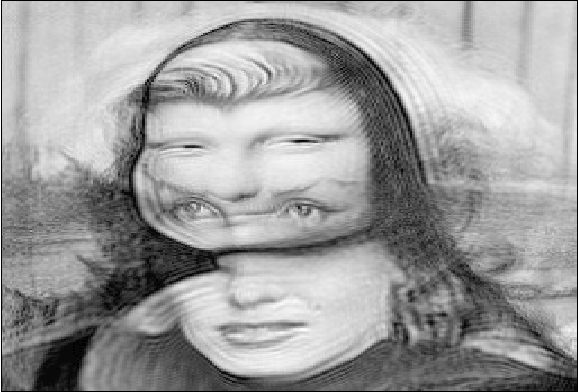
\includegraphics[width=\linewidth]{img/main.png}

\vfill
\begin{minipage}[l]{0.4\textwidth}
\large
\emph{Auteur :}\\
\@author\\
\end{minipage}
\hfill
\begin{minipage}[r]{0.4\textwidth}
\large
\flushright
\emph{A l'attention de :} \\
Carole \textsc{Le Guyader}\\ % Supervisor's Name
Vincent \textsc{Duval}\\
\end{minipage}
\newpage
}
\makeatother
%%%


%\begin{center}
%\vspace{2ex}
%{\huge \textsc{\@title}}
%\vspace{1ex}
%\\
%\linia\\
%\@author \hfill \@date
%\vspace{4ex}
%\end{center}

%\begin{tcolorbox}[enhanced,attach boxed title to top center={yshift=-3mm,yshifttext=-1mm},
 % colback=blue!5!white,colframe=blue!75!black,colbacktitle=red!80!black,
  %title=My title,fonttitle=\bfseries,
  %boxed title style={size=small,colframe=red!50!black} ]
  %This box uses a \textit{boxed title}. The box of the title can
  %be formatted independently from the main box.
%\end{tcolorbox}









\usepackage[toc,page]{appendix}
\renewcommand\appendixtocname{Annexes}
\newcommand{\supp}{\text{supp }}
\newcommand{\prox}{\text{Prox}}
\renewcommand{\div}{\text{div}}
\newcommand{\proj}{\text{Proj}}

\usepackage{subcaption}
\usepackage{multimedia}
\usepackage{afterpage}

\newcommand\blankpage{%
    \null
    \thispagestyle{empty}%
    \addtocounter{page}{-1}%
    \newpage}

\setlength{\parindent}{0pt}
\newcommand\titre{Transport Optimal\\Théorie et Applications}
\newcommand\auteur{Timothée \textsc{Schmoderer}}
\newcommand\dateDoc{2017/2018}
\newcommand\chapitre{Chapitre 2}
\newcommand\cours{Projet de fin d'études}
\usepackage{enumitem}
\everymath{\displaystyle}

\title{\titre }
\author{\auteur}
\date{\dateDoc}

\usepackage{fancyhdr,lastpage}
\pagestyle{fancy}

\lhead{\cours}
\chead{}
\rhead{\currentname}
\lfoot{Théorie du Transport Optimal}
\cfoot{}
\rfoot{Page \thepage\ /\ \pageref*{LastPage}}  


\lstset{
language=Matlab,
}

\hypersetup {
 pdftitle={\titre},    % title
    pdfauthor={\auteur},     % author
    pdfsubject={\cours},   % subject of the document
    pdfkeywords={}, % list of keywords
}


\renewcommand{\lstlistingname}{Code}% Listing -> Code
\renewcommand{\lstlistlistingname}{Liste des \lstlistingname s}% List of Listings -> List of codes



\begin{document}
\afterpage{\blankpage}
\thispagestyle{empty}
\maketitle
\tableofcontents
\newpage


\section{Introduction}

Le présent rapport rend compte du travail effectué pour mon projet de fin d'études (PFE) dans le cadre de mon dernier semestre au département de Génie Mathématique de l'INSA de Rouen Normandie. Le projet proposé, par Carole Le Guyader et Vincent Duval, était de s'attaquer à la découverte de la théorie du transport optimal. Comme nous allons le voir, ce projet m'a amené bien au delà de cette théorie en me faisant explorer la théorie des opérateurs proximaux et en proposant un sérieux défi numérique lors de l'implémentation. \\

Le problème du transport optimal prend ses racines pendant la Révolution française. Un ingénieur français, Gaspard Monge, s'intéresse au problème de transport de ressources d'un site d'extraction à un site de production. Son objectif est de minimiser un coût, que l'on imagine proportionnel à la masse déplacée et à la distance parcourue. C'est le \emph{Mémoire sur la théorie des déblais et des remblais} de 1781 \cite{monge}. La formulation moderne est donnée par un mathématicien russe, Leonid Kantorovitch dans les années 1940. La théorie du transport optimal obtient ses lettres de noblesse dans les années 2000 avec le papier de Jean-David Benamou et Yann Brenier \cite{benamoubrenier}. En explorant un lien, étroit mais pas surprenant, entre la théorie du transport et la mécanique des fluides, ils remettent au gout du jour le problème de transport optimal.\\
\vspace{-0.8cm}
\begin{figure}[!h]
\centering
\begin{subfigure}[b]{0.30\linewidth}
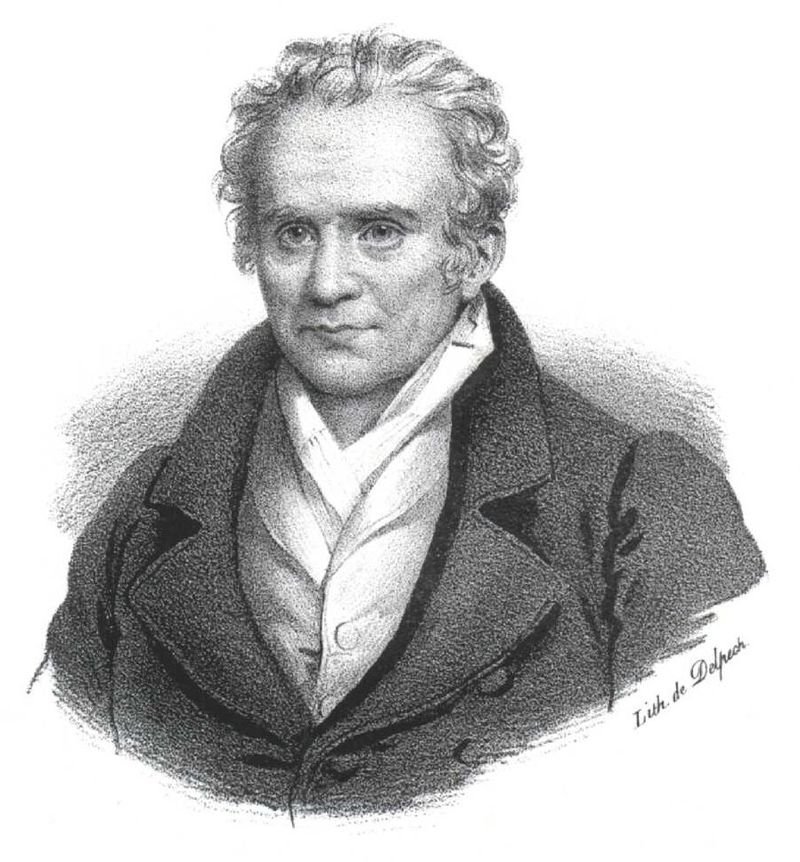
\includegraphics[width=\linewidth]{img/monge.jpg}
\caption*{Gaspard Monge}
\end{subfigure}
\hspace{3cm}
\begin{subfigure}[b]{0.30\linewidth}
\centering
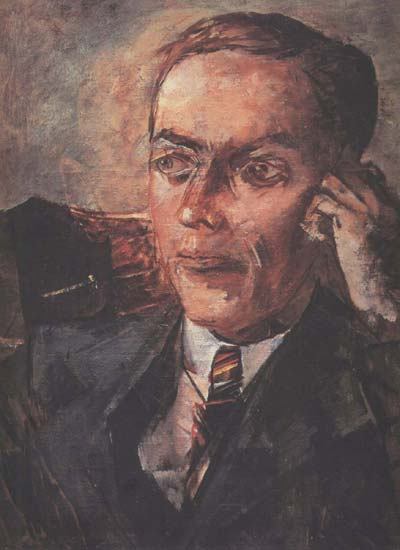
\includegraphics[width=0.8\linewidth]{img/kantorovitch.jpg}
\hspace{-2cm}\caption*{Leonid Kantorovitch}
\end{subfigure}
\caption{Les pères fondateurs de la théorie du transport optimal}
\end{figure}
\vspace{-0.3cm}
%\begin{figure}[!h]
%\centering
%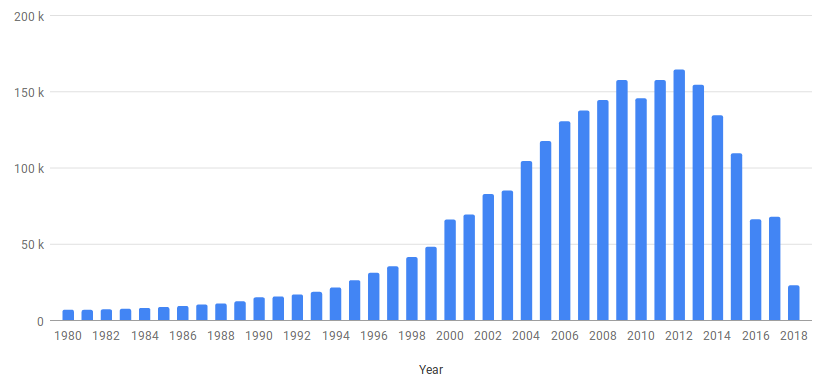
\includegraphics[width=0.8\linewidth]{img/trends.png}
%\caption{Evolution des termes "Optimal Transport" entre 1980 et 2018 sur Google Scholar}
%\end{figure}

Dans ce projet, nous avons étudié, l'article fondateur de Benamou et Brenier, puis nous sommes assez rapidement passés sur l'article de Papadakis, Peyré, Oudet \cite{papadakis} pour la partie numérique. Le projet nous a également emmené voir du côté de l'article de Pesquet et Combettes sur la théorie des opérateurs proximaux \cite{combettes}, et du livre de Santambrogio \cite{santambrogio2015optimal} pour la partie théorique.\\ 

Dans ce rapport, j'ai souhaité être le plus exhaustif possible, la quasi-totalité des énoncés sont démontrés, soit en reprenant des preuves trouvées soit, et ce sera souvent le cas dans la section \eqref{sec:prox}, des preuves que j'ai cherchées moi-même. Ce rapport est organisé comme suit, dans un premier temps nous positionnerons le problème de transport optimal, nous nous attacherons à démontrer l'existence de solutions pour ce problème (en suivant la présentation de Santambrogio, \cite{santambrogio2015optimal}), nous terminerons cette section par démontrer le théorème de Benamou et Brenier qui nous donnera la formulation résolue numériquement par la suite. Dans la seconde partie, nous ferons un détour par la théorie des opérateurs proximaux. Enfin nous discuterons des méthodes numériques mises en œuvre pour résoudre le problème de Benamou et Brenier et nous terminerons par une galerie d'exemples. 

\newpage


\section{Problème de Transport Optimal}
Dans cette section, nous nous attachons à décrire le problème de transport optimal. Nous donnerons des preuves de l'existence de solutions à ce problème. Nous finirons par donner la formulation du problème par Benamou et Brenier, que nous résoudrons numériquement dans la partie \ref{sec:numerique}. 

\subsection{Formulation du problème de Transport Optimal}
Intuitivement, le problème de transport optimal consiste à trouver une méthode pour déplacer un tas de matériaux d'un endroit à un autre, de façon à minimiser un coût, lié au transport de ces matériaux par exemple. C'est l'approche initiale de Monge. 
\begin{figure}[!h]
\centering
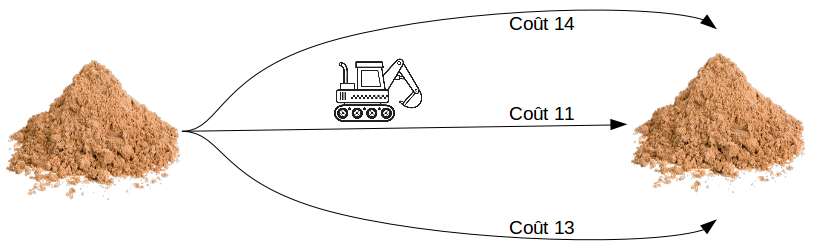
\includegraphics[width=\linewidth]{img/tractopelle.png}
\caption{\label{fig:tractopelle}Le transport optimal dans sa version vulgarisée}
\end{figure}\\
Il faut bien garder en tête cette image, l'application de transport agit comme une petite pelleteuse qui déplace des petits tas de matières sur d'autres petits tas. Suivant le chemin parcouru, ce n'est pas le même coût. \\
Dans des termes plus formels et modernes, les tas de sables représentent des mesures d'ensembles mesurables dans des espaces métriques, le tractopelle est l'application de transport et le coût est la "distance" entre un ensemble de départ et un ensemble d'arrivée. 
\begin{definition}{Transport}
Soient deux mesures de probabilité $\mu$ sur $(\mathcal{X},\mathcal{B}(\mathcal{X}))$ et $\nu$ sur $(\mathcal{Y},\mathcal{B}(\mathcal{Y}))$ munis de leur tribu borélienne. Un \textbf{transport} est une application $T\ :\ \mathcal{X}\rightarrow\mathcal{Y}$ qui envoie la mesure $\mu$ sur la mesure $\nu$. C'est à dire : 
\begin{align}
\forall B\in\mathcal{B}(\mathcal{Y}),\quad \mu(T^{-1}(B))=\nu(B)
\label{eq:trspmesures}
\end{align}
Cela signifie que $\nu$ est la mesure image de $\mu$ par l'application $T$.\\
Nous noterons $T_{\#}\mu=\nu$, une application $T$ vérifiant \eqref{eq:trspmesures}.
\end{definition}
Pour présager du théorème de Benamou et Brenier, remarquons que la relation \eqref{eq:trspmesures} traduit la conservation de la masse par l'application $T$. La figure \ref{fig:illustrans} illustre cette relation dans le cas où les mesures possèdent des densités. Il faut se rendre compte que les figures \ref{fig:tractopelle} et \ref{fig:illustrans} traduisent la même chose. Dans la seconde, l'application prend une petite masse (représentée ici par sa fonction de densité) et l'emmène vers une petite masse de la densité $\nu$. 
\begin{figure}[!h]
\centering
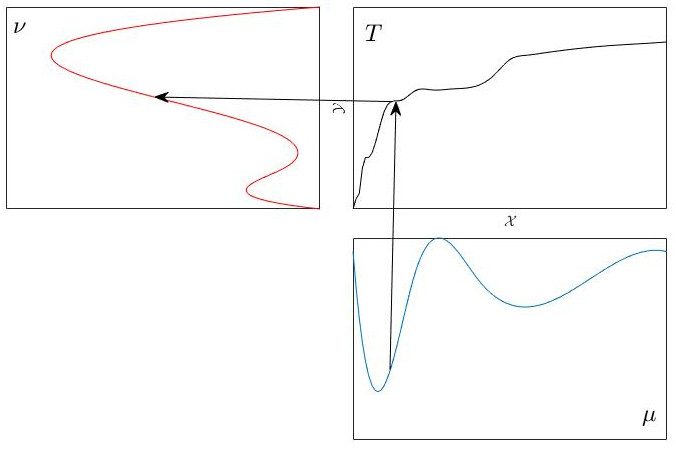
\includegraphics[width=0.7\linewidth]{img/transport.jpg}
\caption{\label{fig:illustrans}Illustration de l'application de transport}
\end{figure}\\
Bien sur, l'application de transport n'est pas unique (cela sera clair lorsque nous regarderons l'équation \eqref{eq:jacobienne}, qui est clairement sous-déterminée), il nous faut alors une manière de sélectionner un transport qui serait "meilleur" que les autres. 

\begin{definition}{}
Le coût est une application 
$$
\fonction{C}{\mathcal{X}\times\mathcal{Y}}{[0,+\infty]}{(x,y)}{C(x,y)}
$$
\end{definition}
Cette application représente le coût d'affecter $x$ en $y$. Ces deux définitions nous amènent au problème de transport optimal : \\

\fbox{
  \parbox{\textwidth}{
  Étant données deux mesures de probabilités $\mu$ sur $\mathcal{X}$, $\nu$ sur $\mathcal{Y}$ et une application coût $C$, trouver une application de transport $T$ réalisant le 
	\begin{equation}
	\tag{MP}
	\inf\left\{M(T) := \int_{\mathcal{X}} C(x,T(x))\ d\mu (x), \quad T_{\#}\mu = \nu\right\}
	\label{eq:MP}
	\end{equation}
  }
}
\vspace{0.3cm}

L'existence du transport optimal n'est absolument pas triviale, nous suivrons la présentation du livre de Santambrogio  \cite{santambrogio2015optimal} pour démontrer l'existence d'une application de transport optimal.\\ 
La méthode que nous suivrons est la suivante. Dans un premier temps nous étudierons une version relaxée de \eqref{eq:MP} sur laquelle l'existence de minimiseurs est plus simple à montrer. Puis par des arguments de dualité, nous verrons sous quelles conditions, l'existence d'une solution de ce problème relaxée nous permet de construire une solution de notre problème de transport optimal. Enfin nous ferrons une petite digression sur le cas où le coût est quadratique avant d'énoncer et démontrer le théorème de Benamou et Brenier. 

\subsection{Plan de Transport Optimal}
Le problème \eqref{eq:MP} est difficile à résoudre du fait de la contrainte. Oublions ce problème pour un temps, et regardons une forme généralisée donnée par Kantorovitch. \\

\fbox{
  \parbox{\textwidth}{
  Étant données deux mesures de probabilités $\mu$ et $\nu$ et un coût $C$, trouver la mesure $\pi$ réalisant le 
	\begin{equation}
	\tag{KP}
	\inf\left\{ K(\pi ) := \int_{\mathcal{X}\times\mathcal{Y}} C(x,y)\ d\pi (x,y), \quad \pi \in\Pi(\mu,\nu )\right\}
	\label{eq:KP}
	\end{equation}
	Où, $\Pi(\mu,\nu)$ est l'ensemble des plans de transports : 
	\begin{empheq}[left={ \Pi(\mu,\nu) = \empheqlbrace}]{align}
	  &  \pi \text{ une probabilité sur }\mathcal{X}\times\mathcal{Y}\nonumber \\
      &  \forall A\in\mathcal{B}(\mathcal{X}),\quad \pi (A\times\mathcal{Y}) = \mu(A) \label{eq:contrKP}\\
      &  \forall B\in\mathcal{B}(\mathcal{Y}),\quad \pi (\mathcal{X}\times B) = \nu(B)  \nonumber,
	\end{empheq}
  }
}
\vspace{0.3cm}

La valeur de $\pi (A\times B)$ décrit la quantité de matière transportée de $A$ en $B$. Cette description permet des déplacements plus généraux qu'un transport classique. En effet, à partir d'un point $x$, les particules peuvent être transportées en plusieurs destinations. Si c'est le cas, alors cela ne peut pas être décrit au travers d'une application de transport $T$, car localement il n'y a pas conservation de la masse.\\
Remarquons que les contraintes \eqref{eq:contrKP} sont des contraintes de marginales sur la mesure de probabilité $\pi$, cela signifie que nous restreignons notre attention aux plans de transports qui déplacent des particules distribuées selon $\mu$ sur des particules distribuées selon $\nu$.

\begin{figure}[!h]
\centering
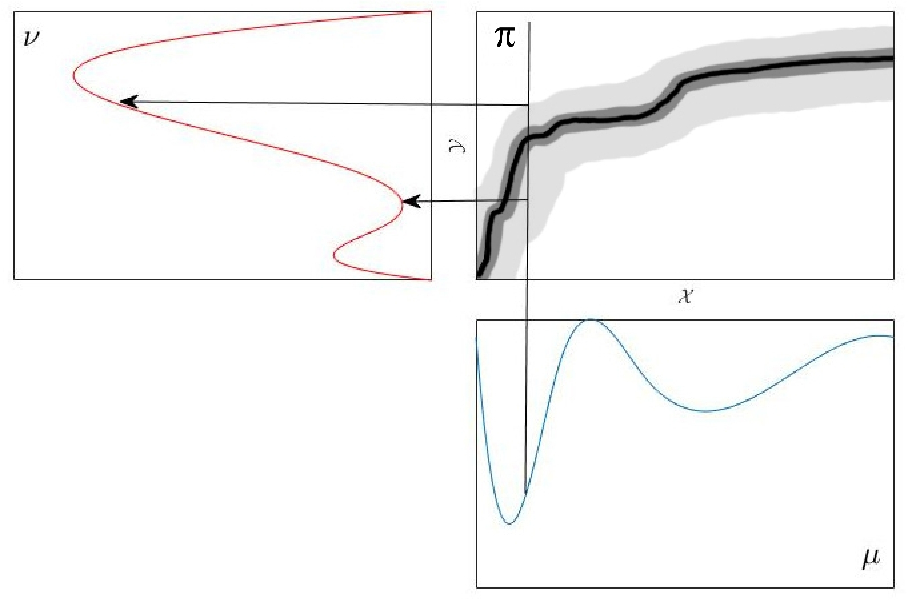
\includegraphics[width=0.6\linewidth]{img/transport_plan2.jpg}
\caption{Illustration de la notion de plan de transport\label{fig:plantransp}}
\end{figure}
La figure \ref{fig:plantransp} illustre la notion de plan de transport. Le dégradé de couleur montre que la mesure $\pi$ peut envoyer un point $x\in\mathcal{X}$ sur plusieurs points de $\mathcal{Y}$ dans différentes proportions. Dans notre analogie avec le tractopelle, cela signifie que les petits tas de sable transportés ne sont plus déposés à un seul endroit mais peuvent être dispersés en plusieurs endroits.\\
Les minimiseurs de ce problème sont appelés plans de transport optimal entre $\mu$ et $\nu$. Ce problème est bien une généralisation de \eqref{eq:MP}, puisque si $\pi = (Id,T)$ pour une certaine fonction mesurable $T\ :\ \mathcal{X}\rightarrow\mathcal{Y}$, alors l'application $T$ serait un transport optimal entre $\mu$ et $\nu$. \\
Nous allons montrer l'existence de solutions pour le problème relaxé \eqref{eq:KP} à l'aide du calcul des variations. Les outils principaux de cette méthode sont rappelés à l'annexe \ref{sec:variations}. 
\begin{theoreme}{}
Soit $\mathcal{X}$ et $\mathcal{Y}$ des espaces métriques compacts. Supposons que le coût $C\ :\ \mathcal{X}\times\mathcal{Y}\rightarrow [0,+\infty]$ soit continue. Alors le problème \eqref{eq:KP} admet une solution.
\end{theoreme}
\begin{preuve}
Il s'agit de montrer que l'ensemble $\Pi (\mu,\nu)$ est compact et que l'application $\pi\rightarrow K(\pi )$ est continue, puis d'appliquer le théorème de Weierstrass \eqref{thm:weierstrass}. \\
Nous choisissons la notion de convergence donnée par la convergence faible des mesures de probabilités (voir \eqref{thm:prokhorov} pour la dualité avec $C_b(\mathcal{X}\times\mathcal{Y})$ ce qui ici, est la même chose que $C(\mathcal{X}\times\mathcal{Y})$ ou $C_0(\mathcal{X}\times\mathcal{Y})$ car $\mathcal{X}$ et $\mathcal{Y}$ sont compacts). Cela nous donne la continuité de $K$ puisque $C\in C(\mathcal{X}\times\mathcal{Y})$. \\

Soit une suite $\pi_n\in\Pi (\mu,\nu )$. Ce sont des mesures de probabilités, donc de masse $1$ et sont donc bornées dans le dual de $C(\mathcal{X}\times\mathcal{Y})$. Ainsi, la compacité faible - * dans les espaces duaux, garanti l'existence d'une sous suite $\pi_{n_k}$ convergeant faiblement vers une probabilité $\pi$. 
Vérifions que $\pi \in \Pi (\mu,\nu )$. \\
Fixons $\phi\in C(\mathcal{X})$, comme $\int\phi\ d\pi_{n_k} =\int \phi\ d\mu $,par passage à la limite, nous avons : $\int\phi\ d\pi =\int\phi\ d\mu$. De même nous montrons que la seconde contrainte de marginale \eqref{eq:contrKP} est vérifiée. \\
Ainsi, l'espace $\Pi(\mu,\nu)$ est compact et le théorème de Weierstrass s'applique.
\end{preuve}

Allons vers plus de généralités. 

\begin{proposition}
Supposons que l'application de coût soit semi continue inférieurement et bornée inférieurement. Alors le problème \eqref{eq:KP} admet une solution. 
\end{proposition}
\begin{preuve}
La seule différence avec le cas précédent est que $K$ n'est plus continue mais semi continue inférieurement pour la convergence faible des mesures de probabilités. Cela vient du lemme suivant appliqué à $f = C$ et $\Omega = \mathcal{X}\times\mathcal{Y}$.
\begin{lemme}
Si $f\ :\ \Omega\rightarrow \RR\cup\{+\infty\}$ est une fonction semi-continue inférieurement, bornée inférieurement sur un espace métrique $\Omega$. Alors la fonctionnel $J \ :\ \mathcal{M}_+(\Omega )\rightarrow \RR\cup\{+\infty\}$ définie sur les mesures de Radon positives par $J(\lambda) =\int f d\lambda$ est semi continue inférieurement pour la convergence faible des mesures. 
\end{lemme}
\begin{preuve}
Soit une suite $(f_k)$ de fonctions continues, bornées convergeant vers $f$ par valeurs croissantes. 
Soit $J_k(\lambda ) =\int f_k\ d\lambda$, $J_k\rightarrow J$ par convergence monotone. Nous pouvons alors écrire $J(\lambda )=\sup_k J_k(\lambda )$.
Alors $J$ est semi-continue inférieurement comme le $\sup$ de fonctionnelles continues.
\end{preuve}
Et donc, le théorème de Weierstrass \eqref{thm:weierstrass} s'applique.
\end{preuve}

\begin{proposition}\label{prop:existKP3}
Supposons que $\mathcal{X}$ et $\mathcal{Y}$ soient des espaces métriques complets et séparables (i.e. polonais) et que le coût $C$ est semi-continue inférieurement et bornée inférieurement. Alors le problème \eqref{eq:KP} admet une solution. 
\end{proposition}
\begin{preuve}
Cette fois, c'est la compacité de $\Pi(\mu,\nu)$ qui est moins évidente. Nous allons utiliser le théorème de Prokhorov \eqref{thm:prokhorov}. Ce qui revient à montrer que toute suite de $\Pi (\mu,\nu)$ est tendue. \\
Soient $\epsilon >0$ et deux compact $K_{\mathcal{X}}\subset\mathcal{X}$ et $K_{\mathcal{Y}}\subset \mathcal{Y}$ tels que $\mu (\mathcal{X}\backslash K_{\mathcal{X}})$, $\nu (\mathcal{Y} \backslash K_{\mathcal{Y}}) < \frac{1}{2}\epsilon$. Cela est possible par la réciproque du théorème de Prokhorov, car une mesure seule est toujours tendue. 
Alors l'ensemble $K_{\mathcal{X}}\times K_{\mathcal{Y}}$ est compact dans $\mathcal{X}\times\mathcal{Y}$, et pour toute suite $\pi_n\in\Pi (\mu,\nu )$, nous avons 
\begin{align*}
\pi_n\left((\mathcal{X}\times\mathcal{Y})\backslash (K_{\mathcal{X}}\times K_{\mathcal{Y}}) \right) &\leq \pi_n((\mathcal{X}\backslash K_{\mathcal{X}})\times \mathcal{Y}) + \pi_n(\mathcal{X}\times (\mathcal{Y}\backslash K_{\mathcal{Y}}))\\
&\leq \mu (\mathcal{X} \backslash K_{\mathcal{X}}) + \nu (\mathcal{Y}\backslash K_{\mathcal{Y}}) < \epsilon
\end{align*}
Ce qui montre la tension et donc la compacité de toute suite de $\Pi (\mu,\nu )$. 
\end{preuve}

\subsection{Problème dual au plan de Transport Optimal}
Maintenant que nous avons démontré l'existence de solution au problème de Kantorovitch, nous souhaiterions savoir sous quelles conditions nous pouvons remonter au problème de Monge. Comme le problème \eqref{eq:KP} est un problème d'optimisation linéaire sous contraintes d'égalité, il est donc naturel d'étudier le problème dual. \\

Toujours suivant la présentation du livre de Santambrogio \cite{santambrogio2015optimal}, cherchons en premier lieu le problème dual formellement. \\
La contrainte $\pi\in\Pi(\mu,\nu)$ peut s'exprimer sous la forme : 
\begin{align}
\sup_{(\phi,\psi)\in C_b(\mathcal{X})\times C_b(\mathcal{Y})}& \int_{\mathcal{X}} \phi(x)\ d\mu (x) + \int_{\mathcal{Y}}\psi(y)\  d\nu(y) - \int_{\mathcal{X}\times\mathcal{Y}}\phi(x)+\psi(y)\ d\pi(x,y)\label{eq:sup1}\\
&= \left\{\begin{array}{cl}
0 & \text{si } \pi \in\Pi(\mu,\nu)\\
+\infty & \text{sinon}
\end{array}\right.\nonumber
\end{align}
Ainsi nous pouvons supprimer la contrainte dans le problème \eqref{eq:KP} en ajoutant l'expression \eqref{eq:sup1}, puisque si la contrainte est satisfaite, rien n'est ajoutée, si elle ne l'est pas nous obtenons $+\infty$ ce qui sera évité par la minimisation. 
$$
\inf_{\pi} \int_{\mathcal{X}\times\mathcal{Y}} C\ d\pi + \sup_{(\phi,\psi)\in C_b(\mathcal{X})\times C_b(\mathcal{Y})} \int_{\mathcal{X}} \phi\ d\mu + \int_{\mathcal{Y}}\psi\  d\nu - \int_{\mathcal{X}\times\mathcal{Y}}\phi(x)+\psi(y)\ d\pi(x,y)
$$
Il n'est pas toujours possible d'échanger le $\sup$ et l'$\inf$, mais supposons pour le moment que cela soit possible : 
\begin{align}
\sup_{(\phi,\psi)\in C_b(\mathcal{X})\times C_b(\mathcal{Y})} \int_{\mathcal{X}} \phi\ d\mu + \int_{\mathcal{Y}}\psi\  d\nu + \inf_{\pi} \int_{\mathcal{X}\times\mathcal{Y}}(C(x,y) - \phi(x)+\psi(y))\ d\pi(x,y)
\label{eq:infsupexchange}
\end{align}

Avec ce problème de maximisation sur les variables $(\phi,\psi)$, l'infimum en $\pi$ peut être réécrit comme une contrainte sur $(\phi,\psi)$ : 
\begin{align}
\inf_{\pi} \int_{\mathcal{X}\times\mathcal{Y}}(C - \phi\oplus\psi) \ d\pi = 
\left\{
\begin{array}{cl}
0 & \text{si } \phi\oplus\psi\leq C \text{ sur } \mathcal{X}\times\mathcal{Y}\\
-\infty &\text{ sinon}
\end{array}
\right.
\end{align}
Où la fonction, $\phi\oplus\psi$ est définie par $(\phi\oplus\psi)(x,y) = \phi(x)+\psi(y)$. L'égalité précédente est justifiée car, si $\phi\oplus\psi>C$ quelque part alors en utilisant des mesures $\pi$ concentrées en cet endroit et de masse croissante, l'intégrale tend vers $-\infty$. Ce qui nous amène au problème suivant : \\

\fbox{
  \parbox{\textwidth}{
  Étant données deux mesures de probabilités $\mu$ et $\nu$ et un coût $C$, trouver deux fonctions continues, bornées $\phi$ et $\psi$ réalisant le 
	\begin{equation}
	\tag{DKP}
	\sup\left\{\int_{\mathcal{X}} \phi\ d\mu + \int_{\mathcal{Y}}\psi\ d\nu, \quad  (\phi,\psi)\in C_b(\mathcal{X})\times C_b(\mathcal{Y}),\quad \phi\oplus\psi \leq C \right\}
	\label{eq:DKP}
	\end{equation}
  }
}
\vspace{0.3cm}

Remarquons que le $\sup\eqref{eq:DKP} \leq \min\eqref{eq:KP}$, en intégrant la condition $\phi\oplus\psi \leq C$ par rapport à $\pi$ : 
$$
\int_{\mathcal{X}} \phi\ d\mu  + \int_{\mathcal{Y}}\psi\ d\nu = \int_{\mathcal{X}\times\mathcal{Y}} \phi\oplus\psi\ d\pi \leq \int_{\mathcal{X}\times\mathcal{Y}} C\ d\pi
$$

Malheureusement le problème \eqref{eq:DKP} n'admet pas trivialement l'existence de ses maximums, car l'espace des fonctions continues bornées n'est pas compact. Nous montrerons dans un premier temps l'existence de ces maximums, puis montrerons que le problème \eqref{eq:DKP} est bien le dual de \eqref{eq:DKP} au sens ou $\max\eqref{eq:DKP} =\min\eqref{eq:KP}$.


\begin{definition}{C et $\bar{C}$-transformée, C et $\bar{C}$-concavité}
Soit une fonction $\chi\ :\ \mathcal{X}\rightarrow [-\infty,+\infty]$. La C-transformée (ou parfois, C - conjuguée) de $\chi$ est définie par $\chi^C\ : \ \mathcal{Y}\rightarrow[-\infty,+\infty]$ : 
$$
\chi^C(y)=\inf_{x\in\mathcal{X}} C(x,y) -\chi(x)
$$
De même, la $\bar{C}$-transformée est définie pour une fonction $\tau\ :\ \mathcal{Y}\rightarrow [-\infty,+\infty]$ par 
$$
\tau^{\bar{C}}(x) = \inf_{y\in\mathcal{Y}} C(x,y) -\tau(y)
$$
De plus, nous dirons qu'une fonction $\psi$ définie sur $\mathcal{Y}$ est $\bar{C}$-concave s'il existe $\chi\ :\ \mathcal{X}\rightarrow [-\infty,+\infty]$ telle que $\psi = \chi^C$. Respectivement, une fonction $\phi$ définie sur $\mathcal{X}$ est dite $C$-concave s'il existe $\tau\ :\ \mathcal{Y}\rightarrow [-\infty,+\infty]$ telle que $\phi=\tau^{\bar{C}}$. \\
Nous noterons $C$-conc($\mathcal{X}$) et $\bar{C}$-conc($\mathcal{Y}$) les ensembles des fonctions $C$ et $\bar{C}$-concaves. 
\end{definition}

Dans notre cas, $C$ est continue sur un ensemble compact, et est donc uniformément continue. C'est à dire qu'il existe une fonction continue croissante $\omega\ :\ \RR^+\rightarrow\RR^+$ et $\omega(0)=0$ (module de continuité) telle que 
$$
\left|C(x,y) - C(x',y')\right| \leq \omega(d(x,x') + d(y,y'))
$$
En reprenant la définition de $\chi^C(y) = \inf_x g_x(y)$ avec $g_x(y) = C(x,y)-\chi(x)$ qui vérifie $|g_x(y)-g_x(y')|\leq\omega(d(y,y'))$. Ce qui montre que $\chi^C$ et $C$ partagent le même module de continuité. \\

Ensuite remarquons qu'étant donnée une paire $(\phi,\psi)$ du problème \eqref{eq:DKP}, elle peut toujours être remplacée par la paire $(\phi,\phi^C)$ puis par $(\phi^{C\bar{C}},\phi^C)$, car les contraintes sont préservées et les intégrales augmentées. 
Nous pourrions espérer itérer ce processus, mais pour toute fonction $\phi$, nous avons $\phi^{C\bar{C}C} = \phi$. Cependant les considérations précédentes nous amènent le théorèmes d'existence suivant. 
\begin{theoreme}{}
\label{thm:existDKP}
Supposons que $\mathcal{X}$ et $\mathcal{Y}$ soient compact et que $C$ est continue. Alors il existe une solution $(\phi,\psi)$ au problème \eqref{eq:DKP}, de la forme $\phi\in C$-conc($\mathcal{X}$), $\psi\in \bar{C}$-conc($\mathcal{Y}$) et $\psi=\phi^C$. En particulier, 
\begin{align}
\max\eqref{eq:DKP} = \max_{\phi\in C\text{-conc}(\mathcal{X})}\int_{\mathcal{X}}\phi\ d\mu +\int_{\mathcal{Y}} \phi^C\ d\nu
\label{eq:existenceDKP}
\end{align}
\end{theoreme}
\begin{preuve}
Prenons une suite maximisante $(\phi_n,\psi_n)$ et améliorons la, par la $C$ et la $\bar{C}$-transformée. Par les considérations précédentes, nous pouvons supposer une borne uniforme sur la continuité de ces fonctions (le même module de continuité que $C$). Gardons la notation $(\phi_n,\psi_n)$  pour désigner cette suite améliorée. \\
Vérifions que cette suite est équibornée pour appliquer le théorème d'Ascoli Arzélà \eqref{thm:ascoli}. Remarquons qu'ajouter une constante à $\phi$ et la retirer à $\psi$ ne change pas la valeur de la fonctionnelle et n'affecte pas les contraintes. Ainsi, comme $\phi_n$ est continue sur un ensemble compact, elle est donc bornée, quitte à ajouter le minimum, nous pouvons supposer que $\min \phi_n=0$, nous avons aussi que $\max \phi_n \leq \omega (d(\mathcal{X}))$, car les oscillations d'une fonction sont toujours plus faible que son module de continuité appliqué à la plus grande distance possible dans l'ensemble.\\
Comme nous avons choisi $\psi_n=\phi_n^C$, nous avons également, $\psi_n(y)=\inf_xC(x,y)-\phi_n(x)\in[\min C- \omega (d(\mathcal{X})),\max C]$. Ce qui nous donne des bornes uniformes sur $(\phi_n,\psi_n)$ et nous permet d'appliquer le théorème d'Ascoli - Arzelà.\\
\`A une sous suite près, $\phi_n\rightarrow\phi$ et $\psi_n\rightarrow\psi$ avec convergence uniforme, de ce fait : 
\begin{align}
\int_{\mathcal{X}}\phi_n\ d\mu + \int_{\mathcal{Y}}\psi_n\ d\nu \rightarrow \int_{\mathcal{X}}\phi\ d\mu + \int_{\mathcal{Y}}\psi\ d\nu
\end{align}
De plus, 
$$
\phi_n(x)+\psi_n(y)\leq C(x,y) \Rightarrow \phi(x)+\psi(y)\leq C(x,y)
$$
Ici la convergence simple aurait suffit. Cela montre que $(\phi,\psi)$ est une paire admissible pour \eqref{eq:DKP} et donc optimale.
\end{preuve}
Avant de montrer que les problèmes \eqref{eq:DKP} et \eqref{eq:KP} sont bien duaux, introduisons un outil, la transformée de Legendre Flenchel et donnons quelques propriétés. 
\begin{definition}{Transformée de Legendre Flenchel}
Pour toute fonction $f\ :\ E\rightarrow \RR\cup\{+\infty\}$ sa transformée de Legendre Flenchel est définie par :
\begin{align}
\fonction{f^{\star}}{E^{\star}}{ \RR\cup\{+\infty\}}{y}{\sup_{x\in E}\langle x,y\rangle -f(x)}
\end{align}
\end{definition}
\begin{propriete}
\begin{enumerate}
\item Une fonction $f$ est convexe et semi continue inférieurement si et seulement si il existe une fonction $g$ telle que $f=g^{\star}$.
\item Une fonction $f\ :\ E\rightarrow \RR\cup\{+\infty\}$ est convexe et semi continue inférieurement si et seulement si $f^{\star\star}=f$.
\end{enumerate}
\end{propriete}
\begin{preuve}
Nous n'entrons pas dans le détail de la preuve, des arguments plus complets peuvent trouvés à ce lien : \url{https://bianchi.wp.imt.fr/files/2015/01/notesMasterBD-2015.pdf} (Proposition 1.4.8)
\begin{enumerate}
\item $\Longleftarrow$ : Il est clair que $=\sup_x \langle x,\cdot \rangle -g(x)$ est dans $\Gamma_0$. \\
$\Longrightarrow$ : Supposons que c'est faux, c'est à dire, $\exists \bar{x}\in\mathcal{D}(f)$ telle que $f(\bar{x})>\bar{z}:=\sup\left\{\langle x_i,\bar{x}\rangle - g_i,\ i\in I\right\}$, où $I$ représente les indices des fonctions qui minorent $f$. Alors le point, $\begin{pmatrix}
\bar{x}\\
\bar{z}
\end{pmatrix}\notin \text{epi}(f)$. On peut alors trouver un hyperplan séparant $\begin{pmatrix}
\bar{x}\\
\bar{z}
\end{pmatrix}$ et $\text{epi}(f)$ pour obtenir une minorante de $f$ contredisant la définition de $\bar{z}$.
\item Il est clair que $f^{\star\star}\leq f$, comme $f\in\Gamma_0$,$\forall x$, nous avons $\partial f(x)\neq \emptyset$. Prenons alors $u\in\partial f(x)$. 
Par l'identité de Flenchel-Young, 
\begin{align*}
f(x) + f^{\star}(x) = \langle u,x\rangle\\
f^{\star\star}(x)+f^{\star}(x)\leq \langle u,x\rangle\\
f^{\star\star}(x)+f^{\star}(x) = \langle u,x\rangle
\end{align*}
Où la dernière égalité vient une fois encore de l'inégalité de Flenchel-Young. Ainsi, 
$$
\left\{
\begin{array}{cl}
f(x) + f^{\star}(x) &= \langle u,x\rangle\\
f^{\star\star}(x)+f^{\star}(x) &= \langle u,x\rangle\\
\end{array}
\right.
$$
Et donc, $f(x)=f^{\star\star}(x)$.
\end{enumerate}
\end{preuve}
\newpage
Montrons à présent que \eqref{eq:DKP} est bien le problème dual associé à \eqref{eq:KP}. 
\begin{theoreme}{}
\label{thm:dualite}
Les problèmes \eqref{eq:KP} et \eqref{eq:DKP} sont bien duaux l'un de l'autre :
\begin{align}
\min\eqref{eq:KP} = \max\eqref{eq:DKP}
\end{align}
\end{theoreme}
\begin{preuve}
Pour tout $p\in C(\mathcal{X}\times\mathcal{Y})$, posons 
$$
H(p) = -\max\left\{\int_{\mathcal{X}} \phi\ d\mu +\int_{\mathcal{Y}} \psi\ d\nu, \quad \phi\oplus\psi\leq C-p\right\}
$$
C'est l'opposée de la valeur de \eqref{eq:DKP} pour le coût $C-p$. Par le théorème \ref{thm:existDKP}, nous avons que, $H(p)$ est bien atteint et que le module de continuité de la paire optimale $(\phi,\psi)$ est le même que celui de $C-p$. 
\begin{lemme}
La fonction $H\ :\ C(\mathcal{X}\times\mathcal{Y})\rightarrow\RR$ est convexe et semi continue inférieurement pour la convergence uniforme.
\end{lemme}
\begin{preuve}
Pour la convexité, prenons $p_0$ et $p_1$ associés avec leur paire optimale $(\phi_0,\psi_0)$ et $(\phi_1,\psi_1)$. Pour $t\in [0,1]$ posons, $p_t=(1-t)p_t+tp_1$, $\phi_t=(1-t)\phi_0 + t\phi_1$ et $\psi_t=(1-t)\psi_0+t\psi_1$. La paire $(\phi_t,\psi_t)$ est admissible dans le maximum définissant $H(p_t)$. Ainsi, 
$$
H(p_t)\leq-\left(\int_{\mathcal{X}}\phi_t\ d\mu+\int_{\mathcal{Y}}\psi_t d\nu\right) = (1-t)H(p_0)+tH(p_1)
$$
Ce qui montre la convexité.\\
Pour la semi continuité, prenons une suite $(p_n)$ convergeant uniformément vers $p$. A une sous suite près, $p_n$ réalise la $\liminf$ de $H(p_n)$. De la convergence uniforme, la suite $p_n$ est équicontinue et bornée (réciproque de théorème d'Ascoli - Arzelà \eqref{thm:ascoli}). Ainsi, les paires optimales correspondantes $(\phi_n,\psi_n)$ sont aussi équicontinues et bornées. A une sous suite près, supposons que $\phi_n\rightarrow\phi$ et $\psi_n\rightarrow\psi$ uniformément. Comme $\phi_n\oplus\psi_n\leq C-p$, nous avons $\phi\oplus\psi\leq C-p$, ainsi :
$$
H(p) \leq - \left(\int_{\mathcal{X}}\phi\ d\mu+\int_{\mathcal{Y}}\psi\ d\nu\right) = \lim_n H(p_n)=\liminf_n H(p_n)
$$
ce qui montre la semi continuité inférieure.
\end{preuve}
Calculons à présent la transformée de Legendre Flenchel de H.\\
$H^{\star}\ :\ \mathcal{M}(\mathcal{X}\times\mathcal{Y})\rightarrow\RR\cup\{+\infty\}$. Pour tout $\pi\in\mathcal{M}(\mathcal{X}\times\mathcal{Y})$, nous avons 
$$
H^{\star}(\pi)= \sup_p \int_{\mathcal{X}\times\mathcal{Y}} p\ d\pi + \sup \left\{ \int_{\mathcal{X}}\phi\ d\mu + \int_{\mathcal{Y}}\psi\ d\nu, \quad \phi\oplus\psi\leq C- p \right\}
$$
Ce qui se réécrit sous la forme d'un $\sup$ unique sur $p,\ \phi,\ \psi$. Remarquons que, si $\pi\notin\mathcal{M}_+(\mathcal{X}\times\mathcal{Y})$, alors il existe $p_0\leq 0$ tel que $\int p_0\ d\pi >0$, en prenant $\phi\equiv 0$, $\psi\equiv 0$ et $p=C+np_0$ en faisant tendre $n$ vers $+\infty$ nous obtenons $H^{\star}(\pi)=+\infty$.\\
D'autre part, si $\pi\in\mathcal{M}_+(\mathcal{X}\times\mathcal{Y})$, en prenant le $p$ le plus grand possible i.e. $p=C-\phi-\psi$, nous obtenons 
$$
H^{\star}(\pi)=  \sup_{(\phi,\psi)} \int_{\mathcal{X}\times\mathcal{Y}} C\ d\pi + \int_{\mathcal{X}}\phi\ d\mu + \int_{\mathcal{Y}}\psi\ d\nu - \int_{\mathcal{X}\times\mathcal{Y}} \phi\ d\pi -\int_{\mathcal{X}\times\mathcal{Y}} \psi\ d\pi
$$
C'est exactement l'expression obtenue au \eqref{eq:sup1} pour réécrire les contraintes de \eqref{eq:KP}. 
$$
H^{\star}(\pi)=\left\{
\begin{array}{cl}
K(\pi) & \text{si } \pi \in\Pi(\mu,\nu)\\
+\infty & \text{sinon}
\end{array}
\right.
$$

La preuve est presque terminée, $\max\eqref{eq:DKP} = -H(0) =- H^{\star\star}(0)$ car $H$ est convexe et semi continue inférieurement. De plus, $H^{\star\star}(0)=\sup_{\pi}\langle 0,\pi\rangle-H^{\star}(\pi)=-\inf H^{\star}=-\min\eqref{eq:KP}$.
\end{preuve}

Ainsi, nous voyons que 
$$
\min\eqref{eq:KP}= \max_{\phi\in C\text{-conc}(\mathcal{X})}\int_{\mathcal{X}}\phi\ d\mu +\int_{\mathcal{Y}} \phi^C\ d\nu
$$
Ce qui montre que la valeur du minimum de \eqref{eq:KP} est une fonction convexe de $\mu$ et $\nu$, comme supremum de fonctionnelle linéaire. 
\begin{definition}{Potentiel de Kantorovitch}
Les fonctions $\phi$ réalisant le maximum de \eqref{eq:existenceDKP} sont appelées potentiels de Kantorovitch pour le transport de $\mu$ sur $\nu$.
\end{definition}

\subsection{Existence du transport optimal}

A partir des résultats précédents sur le problème \eqref{eq:KP} et son dual \eqref{eq:DKP}, nous allons montrer l'existence du transport optimal dans le cas où, $\mathcal{X}=\mathcal{Y}=\Omega\subset\RR^n$ compact et $C(x,y)=h(x-y)$ pour une certaine fonction strictement convexe $h$. 

Rappelons que pour une mesure $\pi$, son support est le plus petit ensemble fermé sur lequel $\pi$ est concentré : 
$$
\supp \pi = \bigcap \left\{A\ |\ A \text{ fermé },\ \pi(\mathcal{X}\backslash A) = 0 \right\}
$$

De l'égalité entre le minimum de \eqref{eq:KP} et le maximum de \eqref{eq:DKP} et le fait que le deux soient atteints, considérons un plan de transport optimal $\pi$ et un potentiel de Kantorovitch $\phi$, 
\begin{align}
\phi(x)+\phi^C(y) &\leq C(x,y) \text{ sur } \Omega\times\Omega \\
\phi(x)+\phi^C(y) &= C(x,y) \text{ sur }\supp\pi
\end{align}
L'égalité vient de l'inégalité (qui est vraie partout) et de 
\begin{align}
\min\eqref{eq:KP} &= \max \eqref{eq:DKP}\nonumber\\
\int_{\Omega\times\Omega} C\ d\pi &= \int_{\Omega}\phi\ d\mu +  \int_{\Omega} \phi^C\ d\nu = \int_{\Omega\times\Omega} \phi\oplus\phi^c\ d\pi
\end{align}
ce qui implique l'égalité $\pi$ presque partout. 

\begin{proposition}
Si $C\in C^1(\Omega\times\Omega,[0,+\infty])$, $\phi$ un potentiel de Kantorovitch pour le coût $C$ dans le transport de $\mu$ vers $\nu$. Soit $(x_0,y_0)\in\supp\pi$. Alors, si $\phi$ est différentiable en $x_0$, nous avons $\nabla\phi(x_0)= \frac{\partial C}{\partial x}(x_0,y_0)$.\\
En particulier les gradients de deux potentiels de Kantorovitch coïncident en tout point $x_0\in\supp\pi$ où ils sont tous les deux différentiables.
\end{proposition}
\begin{preuve}
Soit $(x_0,y_0)\in\supp\pi$ telle que $\phi$ soit différentiable en $x_0$, des calculs précédents, nous déduisons que l'application $x\mapsto\phi(x)-C(x,y_0)$ atteint sont minimum en $x=x_0$. 
Comme $\phi$ et $C(\cdot,y_0)$ sont différentiables, nous obtenons directement le résultat souhaité. 
\end{preuve}


\begin{theoreme}{Existence du transport optimal}
\label{thm:existtrasp}
Soient $\mu$ et $\nu$ des mesures de probabilités sur une domaine compact $\Omega$ de $\RR^n$, alors il existe un plan de transport optimal $\pi$ pour le coût $C(x,y) = h(x-y)$, avec $h$ strictement convexe. \\
De plus, $\pi$ est unique, de la forme $(Id,T)_{\#}\mu$ si $\mu$ est absolument continue et $\partial\Omega$ est $\mu$ - négligeable. Enfin, il existe un potentiel de Kantorovitch $\phi$ qui est lié à $T$ par :
\begin{align}
T(x) = x- (\partial h)^{-1}(\nabla\phi(x))
\end{align}
\end{theoreme}

\begin{preuve}
Le théorème \ref{thm:dualite} nous donne l'existence d'un plan de transport optimal $\pi$ et d'un potentiel de Kantorovitch $\phi$.\\

$\phi$ partage le même module de continuité que $C$, c'est une fonction lipschitzienne sur $\Omega\times\Omega$ puisque $h$ est localement lipschitzienne et bornée sur $\Omega$. Ainsi, $\phi$ est aussi lipschitzienne.\\

Pour $C(x,y) = h(x-y)$,si $h$ est différentiable, nous obtenons par la proposition précédente que $\nabla\phi (x_0)=\nabla h(x_0-y_0)$, si ce n'est pas le cas, nous avons $\nabla\phi(x_0)\in\partial h(x_0-y0)$ le sous différentiel de $h$\footnote{Nous renvoyons à la section \ref{sec:prox} pour plus de détails et de résultats sur les sous-différentiels}. Comme $h$ est strictement convexe, $(\partial h)^{-1}$ existe, et nous avons 
$$
x_0-y_0=(\partial h)^{-1}(\nabla\phi(x_0))
$$
Comme $\mu$ est absolument continue, $\partial\Omega$ et l'ensemble des points où $\phi$ n'est pas différentiable sont négligeables (par le théorème de Rademacher). \\

Cela montre que le plan de transport optimal est induit par un transport, que ce transport est donné par $x\mapsto x -(\partial h)^{-1}(\nabla\phi(x_0))$. Ainsi il est uniquement déterminé, car $\phi$ ne dépend pas de $\pi$. En conséquence, $\pi$ est également unique. 
\end{preuve}
Ainsi, tous les coûts de la forme $C(x,y) =\|x-y\|^p$ avec $p>1$ sont traités. 


\subsection{Le cas quadratique sur $\RR^n$}
Comme souvent le cas quadratique possède quelques propriétés supplémentaires qu'il convient d'exposer. Mettons nous dans $\RR^n $ avec le coût $C(x,y)=\frac{1}{2}\|x-y\|^2$.\\
Premièrement, si nous sommes sur un ensemble compact, nous pouvons préciser le théorème \eqref{thm:existtrasp}. Il existe une application de transport optimal qui s'exprime comme 
$$
T(x) = x -\nabla\phi(x) = \nabla\left(\frac{x^2}{2}-\phi(x)\right) = \nabla u(x)
$$
Pour une certaine fonction convexe $u$. Adaptons le résultat précédent aux domaines non bornés. Considérons pour cela une variante du problème \eqref{eq:DKP} : \\

\fbox{
  \parbox{\textwidth}{
  Étant donné deux mesures de probabilités $\mu$ et $\nu$ et un coût $C$, trouver deux fonctions $\phi$ et $\psi$ réalisant le 
	\begin{equation}
	\tag{DKP - var}
	\sup\left\{\int_{\RR^n} \phi\ d\mu + \int_{\RR^n}\psi\ d\nu, \quad  (\phi,\psi)\in L^1(\RR^n,\mu)\times L^1(\RR^n,\nu),\quad \phi\oplus\psi \leq C \right\}
	\label{eq:DKPvar}
	\end{equation}
  }
}\\

Introduisons un lemme technique établissant un lien entre la $C$ - concavité et la transformée de Legendre Flenchel dans le cas du coût quadratique. 

\begin{lemme}
Soit une fonction $\chi\ :\ \RR^n \rightarrow \RR\cup\{+\infty\}$. Posons, $\fonction{u_{\chi}}{\RR^n}{\RR\cup\{+\infty\}}{x}{\frac{1}{2}\|x\|^2-\chi(x)} $. Alors, $u_{\chi^C} = (u_{\chi})^{\star}$. En particulier, une fonction $\chi$ est $C$ - concave si et seulement si $x\mapsto\frac{1}{2}\|x\|^2-\chi(x)$ est convexe et semi continue inférieurement. 
\end{lemme}
\begin{preuve}
Pour le premier point, calculons 
$$
u_{\chi^C}(x) =\frac{1}{2}\|x\|^2 - \chi^C(x)=\sup_y \frac{1}{2}\|x\|^2  - \frac{1}{2}\|x - y\|^2 + \chi(y) = \sup_y \langle x,y\rangle - \left( \frac{1}{2}\|y\|^2 - \chi(y)\right) 
$$
De plus, comme les fonctions $C$ - concaves sont caractérisées par le fait qu'elles sont des $C$ - transformée et des fonctions convexes semi continues inférieurement (comme le $\sup$ de fonctions affines). Ce qui montre le second point.
\end{preuve}
Nous pouvons à présent énoncer le résultat de dualité. 
\newpage
\begin{theoreme}{}
Soient $\mu$ et $\nu$ des probabilités sur $\RR^n$ et $C(x,y)=\frac{1}{2}\|x-y\|^2$. Supposons que : 
\begin{enumerate}
\item $\int\|x\|^2dx$, $\int\|y\|^2dy<+\infty$,
\item $\mu$ ne donne pas de masse aux hypersurfaces de classe $C^2$.
\end{enumerate}
Alors \eqref{eq:DKPvar} admet une solution $(\phi,\psi)$ et les fonctions $x\mapsto\frac{1}{2}\|x\|^2-\phi(x)$ et $y\mapsto\frac{1}{2}\|y\|^2-\psi(y)$ sont conjuguées l'une de l'autre pour la transformation de Legendre Flenchel.\\
De plus $\sup\eqref{eq:DKPvar}=\inf\eqref{eq:KP}$. 
\end{theoreme}
Comme nous l'avions fait pour \eqref{eq:DKP}, remarquons que $\sup\eqref{eq:DKPvar}\leq \min\eqref{eq:KP}$, en intégrant la condition $\phi\oplus\psi\leq C$ par rapport à $\pi$ : 
$$
\int_{\RR^n}\phi\ d\mu + \int_{\RR^n}\psi\ d\nu = \int_{\RR^n\times\RR^n} \phi\oplus\psi\ d\pi \leq\int_{\RR^n\times\RR^n} C d\pi 
$$


\begin{preuve}
La continuité de $C$ et les propriétés de complétude et de séparabilité de $\RR^n$ nous garantissent l'existence du $\min\eqref{eq:KP}$ par la proposition \eqref{prop:existKP3}. Soit $\pi$ la mesure réalisant ce minimum. \\

Il existe alors une paire $(\phi,\psi)$ avec $\phi$ est $C$ - concave et telle que $\phi(x)+\phi^C(y) = C(x,y)$ pour $(x,y)$ dans le support du plan de transport optimal.\\

Alors, nous déduisons que $x\mapsto\frac{1}{2}\|x\|^2-\phi(x)$ et $y\mapsto\frac{1}{2}\|y\|^2-\psi(y)$ sont convexes, conjuguées l'une de l'autre. En particulier, $\frac{1}{2}\|x\|^2-\phi(x)$ est bornée inférieurement par une fonction linéaire, et donc $\phi$ est bornée supérieurement par un polynôme du second degré. Cela montre que $\phi_+\in L^1(\mu)$ par hypothèse sur $\mu$, de même, nous montrons que $\psi_+\in L^1(\nu)$. \\
Intégrons à présent $\phi\oplus\psi$ par rapport à $\pi$. 
$$
\int_{\RR^n}\phi\ d\mu + \int_{\RR^n}\psi\ d\nu = \int_{\RR^n\times\RR^n}\phi\oplus\psi\ d\pi = \int_{\RR^n\times\RR^n}C\ d\pi \geq 0
$$
Ce qui prouve que $\int_{\RR^n}\phi\ d\mu,\ \int_{\RR^n}\psi\ d\nu > -\infty$ et donc $\phi\in L^1(\mu)$ et $\psi \in L^1(\nu)$.\\

Ainsi, nous pouvons utiliser $(\phi,\phi^C)$ comme paire admissible pour \eqref{eq:DKPvar}. 
$$
\eqref{eq:DKPvar} \geq \int_{\RR^n}\phi\ d\mu + \int_{\RR^n}\phi^C\ d\nu = \int_{\RR^n\times\RR^n}C\ d\pi = \eqref{eq:KP}
$$
par l'optimalité de $\pi$. \\
Ainsi, $\max\eqref{eq:DKPvar} = \min\eqref{eq:KP}$. 
\end{preuve}


\begin{theoreme}{}
Soient $\mu$ et $\nu$ des probabilités sur $\RR^n$ et $C(x,y)=\frac{1}{2}\|x-y\|^2$. Supposons que : 
\begin{enumerate}
\item $\int\|x\|^2dx$, $\int\|y\|^2dy<+\infty$
\item $\mu$ ne donne pas de masse aux hypersurfaces de classe $C^2$.
\end{enumerate}
alors il existe une unique application de transport optimal $T$, donnée par $T=\nabla u$ pour une fonction convexe $u$.
\end{theoreme}

\begin{preuve}
Il existe un plan de transport optimal $\pi$, et par le théorème précédent, une paire $(\phi,\psi)\in L^1(\mu)\times L^1(\nu)$ optimale. \\

Alors comme nous l'avions fait dans le théorème \eqref{thm:existtrasp}, $\pi$ est concentrée sur le graphe de $x\mapsto x-\nabla \phi(x):=\nabla u(x)$, si $u$ (ou de manière équivalente $\phi$) est différentiable, ce que nous allons montrer.\\

Comme $\phi\in L^1(\mu)$, nous en déduisons que $u$ est finie $\mu$ presque partout et comme $u$ est convexe, $\supp\pi\subset \{u<+\infty\}$ est un ensemble convexe.\\
Remarquons que $\partial \{u<+\infty\}$ s'exprime comme le graphe d'une fonction concave, c'est donc une hypersurface de classe $C^2$, qui est $\mu$ négligeable par hypothèse.\\
Dans l'intérieur de $\{u<+\infty\}$, $u$ est différentiable $\mu$ presque partout par hypothèse sur $\mu$ et $u$ convexe.\\
Comme $\phi$ est différentiable $\mu$ presque partout, la mesure $\pi$ est concentrée sur le graphe de $x\mapsto x-\nabla\phi(x)=\nabla u(x)$.
\end{preuve}

Maintenant que nous avons montré l'existence du transport optimal, introduisons petit à petit des hypothèses simplificatrices mais pas aberrantes dans le contexte de la résolution numérique. Mettons nous dans $\RR^n$ et supposons que les mesures aient une densité : $\mu = f_0\ dx$ et $\nu = f_1\ dx$. La relation \eqref{eq:trspmesures} devient alors : 
\begin{align*}
\forall B \in\mathcal{B}(\RR^n),\quad \int_B f_1(y)dy&=\int_{T^{-1}(B)} f_0(x) dx \\
&= \int_B \sum_{x\in T^{-1}(y)} \left(\frac{f_0(x)}{|det\ \nabla T(x)|}\right)dy\\
\end{align*}
C'est à dire $f_1(y) = \sum_{x\in T^{-1}(y)} \left(\frac{f_0(x)}{|det\ \nabla T(x)|}\right)$.\\
Supposons de plus que le transport est injectif et lisse, i.e. $x\in T^{-1}(y) \Leftrightarrow y=T(x)$. Nous obtenons alors l'équation dite de Jacobienne :
 
\begin{equation}
\tag{J}
f_1(T(x)) = \frac{f_0(x)}{|det\ \nabla T(x)|}
\label{eq:jacobienne}
\end{equation}


Notons $\mathcal{T}(f_0,f_1)$ l'ensemble des applications qui vérifient \eqref{eq:jacobienne}.
\begin{definition}{Métrique de Wasserstein}
Pour les coûts de transport de la forme $C(x,y) = \|x - y\|^p$, nous pouvons définir une métrique entre $f_0$ et $f_1$ par
\begin{align*}
W(f_0,f_1)^p=\min_{T\in\mathcal{T}(f_0,f_1)} \int \|x-T(x)\|f_0(x)\ dx
\end{align*} 

\end{definition}


Dans le cas quadratique, $T$ s'écrit comme le gradient d'une fonction convexe, qui satisfait alors l'équation dite de Monge Ampère : 
\begin{equation}
\tag{MA}
f_1(\nabla u(x)) = \frac{f_0(x)}{det\ H u(x)}
\label{eq:mongemapere}
\end{equation}






\subsection{Formulation de J.D. Benamou et Y. Brenier}
Pour le moment, le coût ne dépend que des densités initiale et finale, cependant il semble pertinent de chercher à connaître ce qu'il se passe pendant le transport, cela nous amènera à prendre en compte la notion d'obstacle. 
Dans leur article de 1999, J.D. Benamou et Y. Brenier \cite{benamoubrenier}, ont donné une autre formulation au problème de transport optimal en réintroduisant le temps comme variable. Ils obtiennent alors une interprétation très simple du problème de transport optimal en terme de mécanique des fluides. 

\begin{theoreme}{Benamou, Brenier}
Soient $f_0$ et $f_1$ deux densités de probabilité assez régulières. Alors, 
\begin{align}
\min_{T\in\mathcal{T}(f_0,f_1)} \int\|x-T(x)\|^2dx =\min_{(f,v)\in\mathcal{C}_v}\int_{\RR^n}\int_0^1 f(t,x)\|v(t,x)\|^2dtdx
\end{align}
Avec,
\begin{align*}
f(t,x)\ :&\ \RR\times\RR^n\rightarrow \RR \quad \text{la densité}\\
v(t,x)\ :&\ \RR\times\RR^n\rightarrow \RR^n \quad \text{champ de vecteurs vitesses}
\end{align*}
et 
\begin{align}
C_v=\left\{(f,v)\ |\ \frac{\partial f}{\partial t} + \text{div}_x (fv) =0,\ f(0,\cdot) = f_0,\ f(1,\cdot)=f_1 \right\}
\label{eq:contraintes}
\end{align}
\end{theoreme}
\begin{preuve}
Nous redonnons la preuve donnée par Benamou et Brenier en complétant les points qui nous semble obscurs.\\
Supposons $f_0$ et $f_1$ bornées et à support compact de $\RR^n$. Considérons $(f,v)$, suffisamment régulières, vérifiant \eqref{eq:contraintes}. Cette preuve repose sur l'utilisation des variables lagrangiennes $X(t,x)$ qui décrivent le comportement d'un fluide en "suivant" les particules. 




En termes formels, cela donne, 
\begin{align}
X(0,x)=x\quad\frac{\partial X}{\partial t}(t,x) = v(t,X(t,x))
\label{eq:defcoordlag}
\end{align}
Ainsi, pour toute fonction test $\phi$ :
\begin{align}
\int \phi(t,x)f(t,x)\ dxdt &=\int \phi(t,X(t,x))f_0(x)\ dxdt \label{eq:coordlagrangienn}\\ 
\int \phi(t,x)f(t,x)v(t,x)\ dxdt &= \int \frac{\partial X}{\partial t}(t,x)\phi(t,X(t,x))f_0(x)\ dxdt 
\end{align}
la première égalité vient du changement de variable $x=X(t,x)$, or, $f(t,X(t,x))$ décrit la densité de la particule de fluide déplacée le long du champ de vitesse $v$ à l'instant t, c'est donc la densité initiale en $x$, $f_0(x)$. \\

Remarquons que \eqref{eq:coordlagrangienn} et la condition $f(0,\cdot)=f_0,\ f(1,\cdot) = f_1$ impliquent que $T(x)=X(1,x)$ est un transport valide. En effet, pour tout borélien $B$, $\int_{T(x)\in B}f_0(x)\ dx = \int_{X(1,x)\in B}f_0(x)\ dx$ Ce qui signifie, qu'au temps $1$, la particule $x$ est dans le borélien $B$, comme la densité au temps $1$ est donnée par $f_1$ nous avons bien : $\int_{X(1,x)\in B}f_0(x)\ dx = \int_B f_1(x)\ dx$.


Puis remarquons, en prenant comme fonction test $\phi(t,x) = \|v(t,x)\|^2$ dans \eqref{eq:coordlagrangienn}, que: 
$$
\int_{\RR^n}\int_0^1 f(t,x)\|v(t,x)\|^2\ dxdt = \int_{\RR^n}\int_0^1 f_0(x)\|v(t,X(t,x))\|^2\ dxdt
$$
Nous obtenons, 
\begin{align*}
&= \int_{\RR^n}\int_0^1  f_0(x)\left\|\frac{\partial X}{\partial t} (t,x)\right\|^2dxdt \quad \text{par } \eqref{eq:defcoordlag}\\
&= \int_{\RR^n} f_0(x)\int_0^1 \left\|\frac{\partial X}{\partial t} (t,x)\right\|^2dtdx\\
&\text{par l'inégalité de Jensen : }\\
&\leq \int_{\RR^n} f_0(x)\left\|\int_0^1\frac{\partial X}{\partial t} (t,x) dt \right\|^2dx \\
&\leq \int_{\RR^n} f_0(x)\left\| X(1,x)-X(0,x) \right\|^2dx \\
&\leq \int_{\RR^n} f_0(x)\left\| X(1,x)-x \right\|^2dx  \quad \text{par } \eqref{eq:defcoordlag}\\
\end{align*}

Nous reconnaissons ici la forme qui apparaît dans la distance $L^2$ de Wasserstein, pour le transport $T(x) = X(1,x)$. Prenons $\nabla u(x)$ le transport optimal, nous avons alors :  
$$
\leq \int_{\RR^n} f_0(x)\left\| \nabla u(x)-x \right\|^2dx
$$
Finalement, nous avons montré que : 
$$
\int_{\RR^n}\int_0^1 f(t,x)\|v(t,x)\|^2dxdt \leq \int_{\RR^n} f_0(x)\left\| \nabla u(x)-x \right\|^2dx = d(f_0,f_1)^2
$$
Il reste à trouver un couple $(f,v)$ tel que nous ayons l'égalité et la preuve sera complète. Choisissons $X(t,x) = x+t(\nabla u(x)-x)$, ce qui correspond à la paire $(f,v)$ vérifiant pour toute fonction test $\phi$ : 
\begin{align*}
\int_{\RR^n} \int_0^1 \phi(t,x)f(t,x)\ dtdx &=\int_{\RR^n} \int_0^1 \phi(t, x+t(\nabla u(x)-x)) f_0(x)\ dxdt \\
\int_{\RR^n} \int_0^1 \phi (t,x)f(t,x)v(t,x)\ dtdx &= \int_{\RR^n} \int_0^1 \left(\nabla u (x) - x\right) \phi(t, x+t(\nabla u(x)-x)) f_0(x)\ dtdx
\end{align*}


Et en reprenant le raisonnement de la première étape, nous obtenons
\begin{align*}
\int_{\RR^n} \int_0^1 f(t,x)\|v(t,x)\|^2dtdx &= \int_{\RR^n} \int_0^1 f_0(x)\|v(t,X(t,x)\|^2\\
&= \int_{\RR^n} \int_0^1 f_0(x) \|\frac{\partial X(t,x)}{\partial t}(t,x)\|^2 dtdx \\
&= \int_{\RR^n} f_0(x) \|\nabla u(x) -x\|^2dx \\
\end{align*}
Ce qui achève la preuve. 
\end{preuve}

Remarquons qu'une fois le champ de vitesse $v$ calculé, il est possible de retrouver l'application de transport optimal et intégrant le flot. Plus précisément, soit $x\in \RR^n$, posons $T_t(x)$ satisfaisant 
$$
T_0(x) = x \quad \forall t>0,\ \frac{\partial T_t(x)}{\partial t}=v(T_t(x),t)
$$
Suivant l'idée de Benamou et Brenier, posons le changement de variables $(f,v)\mapsto (f,m)$, où $m=fv$ est la quantité de mouvement. Nous obtenons ainsi un problème d'optimisation convexe sous contraintes linéaires pour la paire $(f,m)$. 

\begin{equation}
\tag{P}
\min_{(f,m)\in \mathcal{C}} \mathcal{J}(f,m)=\int\int_0^1 J(f(x,t),m(x,t))\ dtdx
\label{eq:pbm}
\end{equation}

\begin{align}
\forall (m,f)\in \RR^n\times\RR, \quad J(m,f) = \left\{\begin{array}{cl}
\frac{\|m\|^2}{2f} & \text{si } f>0 \\
0 &\text{si } (m,f) = (0,0)\\
+\infty & \text{sinon} 
\end{array}\right.
\end{align}

\begin{equation}
\tag{C}
\mathcal{C}=\left\{(m,f)\ |\ \frac{\partial f}{\partial t} + \div_x(m)=0\quad f(\cdot,0)=f_0,\ f(\cdot,1)=f_1\right\}
\label{eq:constraint}
\end{equation}

\newpage
\section{Optimisation convexe non différentiable}
\label{sec:prox}
Dans la section précédente, nous avons montré l'existence de solutions à notre problème de transport optimal, nous avons introduit la formulation de Benamou et Brenier. C'est pour cette formulation que nous développerons des algorithmes de résolution numérique. Cependant, avant de présenter ces algorithmes de résolution numérique, nous présentons la théorie des opérateurs proximaux qui joueront un rôle central dans notre modèle. \\

L'opérateur proximal d'une fonction convexe généralise la notion de projection sur un ensemble convexe. Cette notion fût introduite pour répondre aux problèmes de minimisation de fonctions non nécessairement différentiables. 

Suivant la présentation de \emph{P.L. Combettes \emph{et} J.C. Pesquet} \cite{combettes} nous présentons une série de résultats sur les opérateurs proximaux, en complétant quelques preuves.
\paragraph{Notation :}Le domaine d'une fonction $f:\ \RR^n\longrightarrow\ ]-\infty,+\infty]$ est $\mathcal{D}(f) = \{ x\in\RR^n\ |\ f(x) < +\infty \} $. Notons $\Gamma_0(\RR^n)$ l'ensemble des fonctions convexes semi-continues inférieurement à valeurs dans $]-\infty,+\infty]$ telles que $\mathcal{D}(f) \neq \emptyset$. 
\subsection{Sous - différentiel}
Commençons par introduire une notion de différentiation plus faible. 
\begin{definition}{Sous - différentiel}
Soit $f\in\Gamma_0(\RR^n)$, le sous - différentiel de $f$ est l'application suivante,
$$
\fonction{\partial f}{\RR^n}{\mathcal{P}(\RR^n)}{x}{\left\{ u\in\RR^n\ |\ \forall y\in\RR^n,\ \langle u,y-x\rangle +f(x)\leq f(y) \right\}}
$$ 
Avec $\mathcal{P}(\RR^n)$, l'ensemble des parties de $\RR^n$.
\end{definition}


L'interprétation géométrique du sous-différentiel est la suivante. Il est formé par toutes les directions des hyperplans qui passent par le point $(x,f(x))$ et restent "sous" le graphe de la fonction $f$. \\

\exemple{Calculons le sous différentiel en tout point de 
$$
\fonction{f}{\RR}{\RR^+}{x}{|x|}
$$
Considérons deux cas, 
\begin{enumerate}
\item $\mathrm{x>0}$ (le cas $x<0$ est identique). Soit une direction $u$ appartient au sous différentiel de $f$ en x, alors $\forall y\in \RR$ : 
\begin{align*}
u(y-x) + f(x) \leq f(y)\\
u(y-x) + x \leq |y|\\
\end{align*}
En particulier, pour $y = 0$ nous obtenons $x(1-u) \leq 0$, ainsi $u\geq 1$. Et en prenant $y > x$ (en particulier, $y>0$) nous obtenons $u(y-x) + x \leq y$, ce qui implique $u\leq 1$et donc $u=1$
\item $\mathrm{x=0}$ Soit $u\in \partial f(0)$, alors $u$ doit vérifier pour tout $y\in \RR$,
\begin{align*}
uy\leq |y|
\end{align*}
En prenant $y>0$ nous obtenons que $u\leq 1$ et en prenant $y<0$, nous avons $u\geq -1$.
\end{enumerate}
En somme, 
$$
\partial f(x) =
\left\{
\begin{array}{cc}
\{-1\} & x <0 \\
\left[-1,1\right] & x =0\\
\{1\} & x>0\\
\end{array}
\right.
$$
Ce qui correspond bien à l'interprétation géométrique donnée et à la figure \ref{fig:subgradient}.
\begin{figure}[!h]
\centering
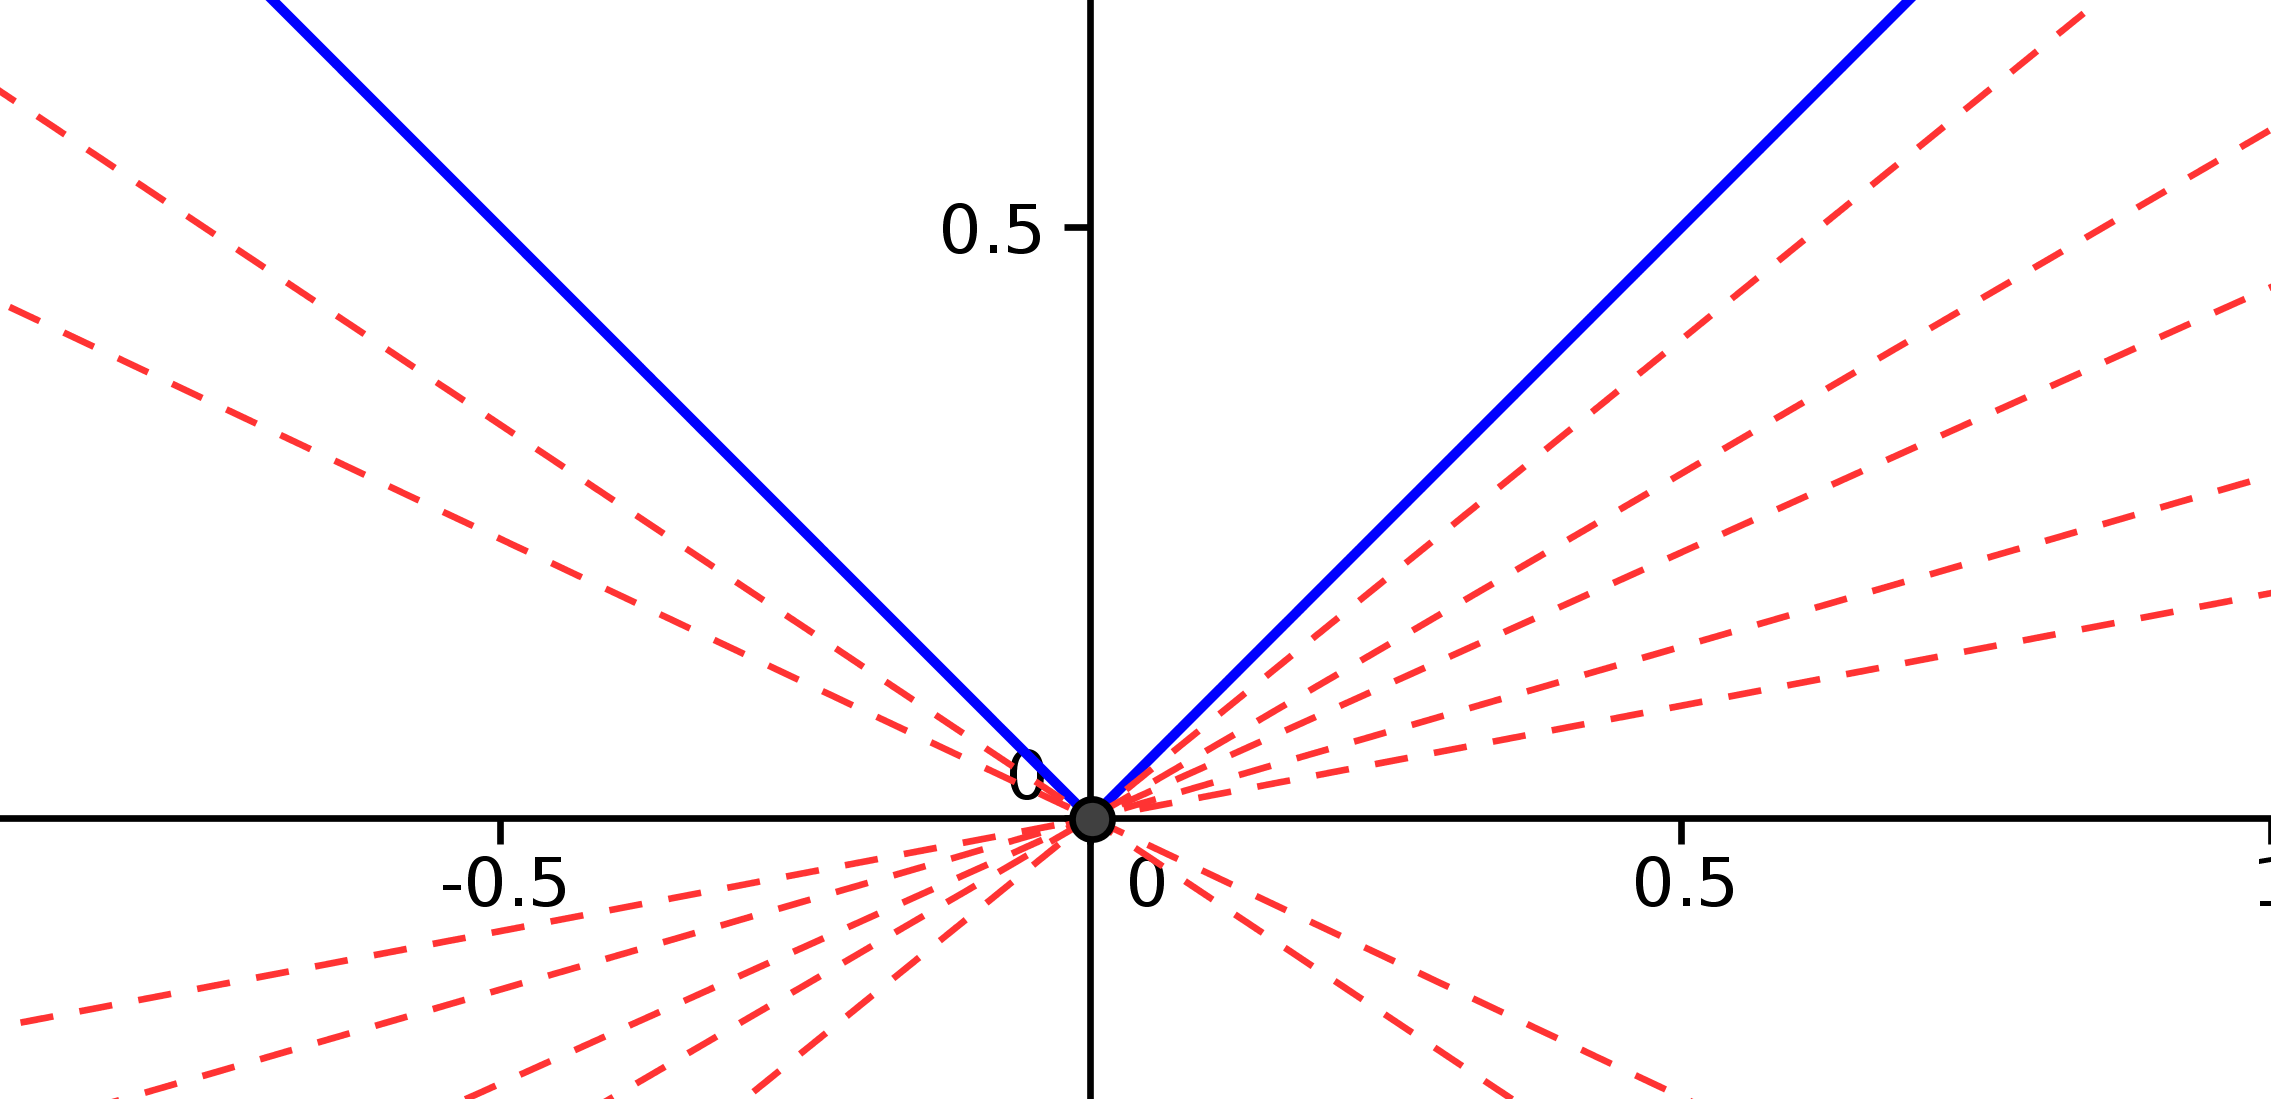
\includegraphics[scale=0.6]{img/sub_gradient.png}
\caption{\label{fig:subgradient}Illustration du sous - différentiel de $|x|$ en $0$}
\end{figure}
}

\begin{propriete}
Soit $f\in\Gamma_0(\RR^n)$. Si $f$ est différentiable sur son domaine, alors 
$$
\forall x\in \mathcal{D}(f)^{\circ},\ \partial f(x) = \{\nabla f(x)\}
$$
\end{propriete}
\begin{preuve}
Comme une $f$ est convexe différentiable, nous avons la caractérisation suivante du gradient : 
$$
\forall x,y\in\RR^n,\quad \langle \nabla f (x) ,y-x\rangle +f(x) \leq f(y)
$$
qui implique que $\nabla f(x) \in\partial f(x)$.\\
Supposons à présent que $p\in\partial f(x)$. Soit une suite $y_n^1$ de $\RR^n$ qui tend vers x. Écrivons, $y_n^1=x+k_n$ avec $\|k_n\|\rightarrow 0$. Posons alors $y_n^2$ une seconde suite de $\RR^n$ telle que $y_n^2= x-k_n$, alors : 
$$
\left\{
\begin{array}{cc}
\langle p, k_n\rangle &\leq f(x +k_n) - f(x) \\
\langle p,-k_n\rangle & \leq f(x-k_n)-f(x) \\
\end{array}
\right.
$$
Comme $f$ est différentiable dans son domaine, nous pouvons écrire, 
$$
f(x\pm k_n)=f(x) \pm \langle \nabla f(x), k_n\rangle
$$
Ainsi, nous obtenons
$$
\left\{
\begin{array}{cc}
\langle p, k_n\rangle &\leq \langle \nabla f(x), k_n\rangle \\
\langle p, k_n\rangle &\geq \langle \nabla f(x), k_n\rangle \\
\end{array}
\right.
$$
Ainsi $\langle p,k_n \rangle = \langle \nabla f(x),k_n\rangle$. En faisant tendre $n$ vers $+\infty$, comme la suite $k_n$ converge fortement vers $0$, elle va aussi converger faiblement. Ce qui implique que $p=\nabla f(x)$. 
\end{preuve}
Cette propriété est cohérente avec l'exemple précédent, $\partial f(x) =f'(x)$ partout où $f$ est différentiable, c'est à dire $x\neq 0$. 

\begin{propriete}
Si $f = \alpha f_1+\beta f_2$, avec $f_1,\ f_2,\ \alpha f_1+\beta f_2\in\Gamma_0(\RR^n)$ et $\alpha,\ \beta \geq 0$. Alors 
\begin{align*}
\partial f(x) &= \alpha \partial f_1(x) + \beta \partial f_2(x) \\
&= \left\{u\in\RR^n\ |\ \exists (u_1,u_2)\in \partial f_1(x)\times f_2(x),\ u = \alpha u_1 + \beta u_2 \right\}
\end{align*}
\end{propriete}
\begin{preuve}
\vspace{-1cm}
\paragraph{$\alpha\partial f_1(x) +\beta \partial f_2(x) \subset
\partial (\alpha f_1 +\beta f_2)(x)$ :}$u\in\RR^n$ est dans $\partial (\alpha f_1 +\beta f_2)(x)$ si et seulement si pour tout $y\in \RR^n$, nous avons 
$$
\langle u,y-x\rangle + \alpha f_1(x) +\beta f_2(x) \leq  \alpha f_1(y) +\beta f_2(y) 
$$
En particulier en prenant $u\in \alpha\partial f_1(x) +\beta \partial f_2(x) $, au sens donné dans la propriété, cette inégalité est vérifiée. \\

L'inclusion inverse demande plus de travail et des notions non introduites ici. Elle peut être trouvée à \url{https://maunamn.wordpress.com/8-the-subdifferential-sum-rule/} (théorème 8.2).

%\paragraph{$\alpha\partial f_1(x) +\beta \partial f_2(x) \supset
%\partial (\alpha f_1 +\beta f_2)(x)$ :}Soit $u\in\partial (\alpha f_1 +\beta f_2)(x)$, par contradiction, supposons que  $u\notin \alpha\partial f_1(x) +\beta \partial f_2(x)$, c'est à dire : 
%$$
%\forall (u_1,u_2)\in \partial f_1(x) \times \partial f_2(x),\quad u\neq \alpha u_1+\beta u_2
%$$
%{\Huge EMPTY}
\end{preuve}
\exemple{Calculons le sous différentielle de $P:x\mapsto f(x)+\frac{1}{2}\|x-y\|^2$, pour une certaine fonction $f\in\Gamma_0(\RR^n)$ et $y\in\RR^n$ fixé. \\
Par la propriété précédente, 
$$
\partial P(x)=\partial f(x)+\partial(\frac{1}{2}\|\cdot\|^2)(x)
$$
Comme la norme 2 est différentiable, $\partial(\frac{1}{2}\|\cdot-y\|^2)(x) = \{x-y\}$. Ainsi, 
$$
\partial P(x)=\partial f(x)+\{x-y\}
$$
Où la somme est entendue dans un sens ensembliste. 
}

La notion de sous - différentiel est centrale car elle permet de caractériser les minimiseurs d'une fonction (même non différentiable).
\begin{theoreme}{}
Soit $f\in\Gamma_0(\RR^n)$. Le point $x^{\star}\in\RR^n$ est un point de minimum global de $f$ si et seulement si 
$$
0\in \partial f(x^{\star})
$$ 
\end{theoreme}
\begin{preuve}
\vspace{-1cm}
Soit $x^{\star}$ le minimum global de $f$, 

\begin{align*}
\Longleftrightarrow \quad & \forall y\in\RR^n\quad  f(x^{\star})                        \leq f(y)\\
\Longleftrightarrow \quad &                  \langle 0,y-x\rangle +f(x^{\star})  \leq f(y)\\
\Longleftrightarrow \quad &                   0\in \partial f(x^{\star})       
\end{align*}

\end{preuve}
\subsection{Opérateur proximal}
L'opérateur proximal est un outil important dans l'optimisation de fonctions convexes non différentiables. C'est une application minimisant une fonction fortement convexe dépendant de la fonction originale $f$. En trouvant un compromis entre atteindre le minimum de la fonction non différentiable $f$ et en forçant une proximité avec l'argument, nous approchons le minimum de $f$. 

\begin{definition}{Opérateur proximal}
Soit $f\in\Gamma_0(\RR^n)$. L'opérateur proximal de $f$, noté $\prox_f$, est défini pour tout $x\in\RR^n$ par : 
$$
\prox_f(x) = \argmin_{y\in\RR^n} f(y) +\frac{1}{2}\|x-y\|^2
$$
\end{definition}
\exemple{Prenons, l'indicatrice d'un ensemble convexe non vide $C$ : 
$$
\iota_C = \left\{
\begin{array}{cc}
0 & x\in C\\
+\infty & x \notin C
\end{array}
\right.
$$
Alors, 
\begin{align*}
\prox_{\iota_C}(x) &= \arg \min_{y\in\RR^n} \iota_C(y) + \frac{1}{2}\|x-y\|^2\\
&= \arg\min_{y\in C} \frac{1}{2}\|x-y\|^2\\
&= \mathrm{P}_C (x)\\ 
\end{align*}
Où, $\mathrm{P}_C$ désigne la projection orthogonale sur $C$. 
}\\

Sur la figure \ref{fig:proximal} (tirée de \cite{parikh2014proximal}), nous avons en \textbf{gras} la frontière de la fonction $f$, les lignes fines sont les lignes de niveaux de $f$. Nous évaluons $\prox_f$ sur les points bleus ce qui les associent aux points rouges correspondant. Les trois points dans le domaine restent dans le domaine et se déplacent vers le minimum, et les deux à l'extérieur du domaine se placent sur la frontière de celui-ci en direction du minimum. 
\begin{figure}[!h]
\centering
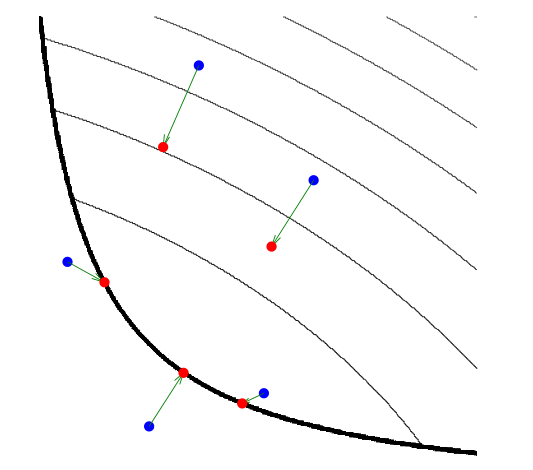
\includegraphics[scale=0.7]{img/proximal.png}
\caption{\label{fig:proximal}Illustration de l'opérateur proximal}
\end{figure}\\

\newpage
Un scalaire $\gamma >0 $ peut être introduit dans cette définition $\prox_{\gamma f}$, ce paramètre contrôle le poids apporté à la minimisation de $f$. Un $\gamma$ grand, forcera de se rapprocher fortement du minimum de $f$, alors qu'un $\gamma$ petit favorisera les points proches de $x$.\\
Le résultat important de la théorie des opérateurs proximaux est le suivant. 
\begin{propriete}
Soit une fonction $f\in\Gamma_0(\RR^n)$. Alors, $\prox_f(x)$ existe et est unique pour tout $x\in\RR^n$.\\
De plus, il est caractérisé par : 
$$
\forall (x,p)\in \RR^n\times\RR^n\quad p=\prox_fx\quad\Longleftrightarrow\quad x-p\in\partial f(p)
$$
En particulier, si $f$ est différentiable alors : 
$$
\forall (x,p)\in \RR^n\times\RR^n\quad p=\prox_fx\quad \Longleftrightarrow \quad x-p=\nabla f(p)
$$
\end{propriete}
\begin{preuve}
$\forall x \in \RR^n$, la fonction $g\ :\ y \rightarrow f(y) +\frac{1}{2}\|x-y\|^2$ est strictement convexe et dans $\Gamma_0(\RR^n)$ (i.e. non identiquement égale à $+\infty$). Ce qui montre que le minimum de $g$ est toujours atteint et est unique. 


\paragraph{$\Leftarrow$} Supposons que $x-p\in\partial f(p)$. Alors, pour tout $y\in\RR^n$, nous avons 
$$
\langle x-p,y-p\rangle +f(p) \leq f(y)
$$
Or,
\begin{align*}
\langle x-p,y-p\rangle &= \frac{1}{2}\langle x-p,y-x+x-p\rangle + \frac{1}{2}\langle  x-y+y-p,y-p\rangle\\
&=\frac{1}{2} \|x-p\|^2 + \frac{1}{2}\|y-p \|^2 +\frac{1}{2}\left( \langle x-p,y-x\rangle + \langle x-y,y-p\rangle\right)\\
&= \frac{1}{2} \|x-p\|^2 + \frac{1}{2}\|y-p \|^2 -\frac{1}{2}\|x-y\|^2
\end{align*}
Ainsi, $\forall y\in\RR^n$ :
\begin{align*}
\frac{1}{2} \|x-p\|^2 + \frac{1}{2}\|y-p \|^2 -\frac{1}{2}\|x-y\|^2 + f(p) &\leq f(y) \\
\frac{1}{2} \|x-p\|^2 + f(p) &\leq f(y) + \frac{1}{2}\|x-y\|^2\\
\end{align*}
Donc $p=\prox_f(x)$.
\paragraph{$\Rightarrow$} Soit $(x,p)\in \RR^n\times\RR^n$ telle que $p=\prox_f(x)$. Cela signifie que $p$ minimise l'application $y\mapsto f(y)+\frac{1}{2}\|x-y\|^2$, par la caractérisation du minimum par le sous différentiel, $0\in\partial \left(f(\cdot)+\frac{1}{2}\|x-\cdot\|^2 \right)(p)$. Par la règle de la somme des sous différentielles et l'exemple, $\exists u\in\partial f(p)$ telle que $0=u+(p-x)$. \\
Ainsi, $u=x-p\in\partial f(p)$. 
\end{preuve}
 
De plus, 
\begin{propriete}
Le point $x^{\star}$ minimise $f$ si et seulement si 
$$
x^{\star} = \prox_f(x^{\star})
$$
\end{propriete} 
\begin{preuve}
\vspace{-1cm}
\paragraph{$\Rightarrow$} Supposons que $x^{\star}$ minimise $f$ alors, $\forall y\in\RR^2$,
$$
f(x^{\star}) +\frac{1}{2}\|x^{\star}-x^{\star}\|^2 = f(x^{\star})\leq f(y)\leq f(y)+\frac{1}{2}\|x^{\star}-y\|^2
$$
Donc, $\prox_f(x^{\star}) = x^{\star}$.
\paragraph{$\Leftarrow$} Utilisons la caractérisation de minimisation donnée par le sous - différentiel. Le point $\tilde{x}$ minimise $x\mapsto f(x) +\frac{1}{2}\|x-y\|^2$, c'est à dire $\tilde{x} = \prox_f(y)$, si et seulement si 
$$
0\in \partial f(\tilde{x}) + \{\tilde{x}-y\}
$$
Par l'exemple précédent. \\
Prenons $y=\tilde{x}:=x^{\star}$, alors nous obtenons $0\in\partial f(x^{\star})$. Et donc $x^{\star}$ minimise $f$.
\end{preuve}

Cela suggère des algorithmes de point fixe pour approcher le minimum de $f$. 

%Cela fonctionnerait si $\prox_f$ était une contraction (i.e. c - lipschitzienne, $0<c<1$). Ce n'est pas le cas, cependant nous avons une propriété de non expansivité qui est suffisante pour une itération de point fixe : 
%$$
%\|prox_f(x)-prox_f(y)\|^2\leq \langle prox_f(x)-prox_f(y),x-y\rangle
%$$
%C'est un cas particulier d'opérateur non expansif (comme par exemple, $-Id$ ou les rotations, \cite{browder1965nonexpansive,brezis1973ope}). 
%\begin{definition}{Application non expansive}
%Une application $N:\ \RR^n\rightarrow \RR^n$ est dite non expansive si 
%$$
%\forall (x,y)\in\RR^n\times\RR^n,\quad \|N(x)-N(y)\| \leq \|x-y\|
%$$
%C'est à dire que $N$ est 1-lipschitzienne. Nous avons la caractérisation suivante, $N$ est non expansive si et seulement si 
%$$
%\forall (x,y)\in\RR^n\times\RR^n,\quad \|N(x)-N(y)\|^2 \leq  \langle N(x)-N(y),x-y\rangle
%$$
%\end{definition}
%
%Si $N$ est un opérateur non expansif alors $\forall \alpha \in ]0,1[$ l'opérateur $T = (1-\alpha)I + \alpha N$ a les mêmes poinst fixes que $N$, et qu'en itérant $T$, il y a convergence vers les poinst fixes. C'est à dire, la suite 
%$$
%x_{n+1} = (1-\alpha )x_n +N(x_n)
%$$
%converge vers un point fixe de $N$.
 
Regardons le problème de minimisation suivant, cette forme nous intéressera particulièrement dans la suite, \\

\fbox{
  \parbox{\textwidth}{
  Soient $f_1$ et $f_2$ deux fonctions de $\Gamma_0(\RR^n)$ telles que $f_1+f_2\in\Gamma_0(\RR^n)$, en particulier le support de $f_1+f_2$ est non vide. Supposons que
  $$
  \lim_{\|x\|\rightarrow+\infty} f_1(x)+f_2(x) =+\infty
  $$
Considérons alors le problème de minimisation, 
Trouver $x\in\RR^n$ qui réalise le 
\begin{align}
\min_{x\in\RR^n}f_1(x)+f_2(x)
\label{eq:pbmminimi}
\end{align}
  }
}

\begin{propriete}
Le problème \ref{eq:pbmminimi} admet une solution et pour tout $\gamma >0$, elle est caractérisée par :
$$
\left\{
\begin{array}{rcl}
x^{\star} &= & \prox_{\gamma f_2} y \\
\prox_{\gamma f_2}y &= & \prox_{\gamma f_1}(2\prox_{\gamma f_2}y -y)
\end{array}
\right.
$$
\end{propriete}

\begin{preuve}
Omettons le paramètre $\gamma$ qui ne change rien à la preuve. $f_1+f_2$ est une fonction convexe, infinie à l'infini donc l'existence d'un minimiseur est immédiate.
\begin{align*}
x^{\star} =\argmin_x f_1(x) + f_2(x) &\Longleftrightarrow 0\in \partial (f_1+f_2)(x^{\star}) \\
&\Longleftrightarrow \exists (x_1,x_2)\in \partial f_1(x^{\star})\times\partial f_2(x^{\star}) \text{ telle que } 0=x_1+x_2
\end{align*}
Prenons  $y$ tel que $x_1=x^{\star} - y$, ainsi $x^{\star}-y\in \partial f_1(x^{\star})$ et $y-x^{\star}\in\partial f_2(x^{\star})$.
\begin{align*}
&\Longleftrightarrow x^{\star} =\prox_{f_2} (y) \text{ et } (2x^{\star}-y)-x^{\star}\in\partial(f_1)(x^{\star})\\
&\Longleftrightarrow x^{\star} =\prox_{f_2} (y) \text{ et } x^{\star}=\prox_{f_1}(2x^{\star}-y)
\end{align*}
\end{preuve}

Suivant les idées d'algorithmes de point fixe sur les opérateurs proximaux, nous introduisons l'algorithme suivant dit de \emph{Douglas - Rachford}.
\begin{algorithm}
\caption{Douglas-Rachford}
\begin{algorithmic}
\STATE Soient $\gamma >0$ et $y_0\in \RR^n$
\FOR{$n=0,\ 1,\ \ldots$}
\STATE $x_n = \prox_{\gamma f_2} y_n$
\STATE $\lambda_n \in ]0,2[$
\STATE $y_{n+1} = y_n + \lambda_n(\prox_{\gamma f_1} (2x_n-y_n)-x_n)$
\ENDFOR
\end{algorithmic}
\end{algorithm}

\begin{propriete}
Toute suite $(x_n)$ générée par l'algorithme de Douglas - Rachford converge vers une solution du problème \ref{eq:pbmminimi}.
\end{propriete}

\begin{preuve}
L'itération sur $y_n$ peut se réécrire comme une opération de point fixe, $y_{n+1}=F(y_n)$, avec $F:y\mapsto y+\prox_{ f_1}(2\prox_{f_2}(y)-y)-\prox_{f_2}(y)$.\\
Montrons que $y$ est un point fixe de $F$ si et seulement si $x=\prox_{f_2}(y)$ satisfait $0\in\partial f_1(x)+\partial f_2(x)$, i.e. :
$$
y=F(y) \Longleftrightarrow 0\in\partial f_1(\prox_{f_2}(y))+\partial f_2(\prox_{f_2}(y))
$$ 

Calculons, 
\begin{align*}
x=\prox_{f_2}(y) &,\quad y = F(y) \\
\Longleftrightarrow\quad x=\prox_{ f_2}(y) &,\quad x = \prox_{f_1}(2x-y) \\
\Longleftrightarrow\quad y-x\in\partial f_2(x)   &, \quad x-y\in\partial f_1(x)
\end{align*}
Alors, si $y=F(y)$, cela implique que $x=\prox_{f_2}(y)$ vérifie 
$$
0=(y-x)+(x-y)\in \partial(f_1+f_2)(x)
$$
Réciproquement, si $z\in\partial f_1(x)$ et $-z\in\partial f_2(x)$, alors $y=x-z$ est un point fixe de $F$. Ce qui montre le résultat annoncé.\\
La continuité des $\prox$ entraînant celle de $F$, la suite $y_n$ converge. Et donc $x_n$ converge également et vers un minimum du problème \eqref{eq:pbmminimi}.\\

Le paramètre $\lambda_n$, relaxe l'équation de point fixe : $y_{n+1}=y_n + \lambda_n(F(y_n)-y_n)$. 
\end{preuve}






\newpage

\section{Méthode numérique}
\label{sec:numerique}
Dans cette section, nous présentons différentes manières d'approcher numériquement la solution du problème \eqref{eq:MP}. La méthode consiste principalement à trouver une manière efficace de calculer les contraintes. Nous présentons la méthode implémenté par Papadakis et al. dans \cite{papadakis}. Cette méthode repose sur l'utilisation de grilles décentrées pour obtenir de bonnes approximations des dérivées. Cependant, je tiens à souligner que le déploiement de cette artillerie n'est pas nécessaire à la résolution numérique du problème, par exemple une méthode plus simple est présentée ici\footnote{\url{http://www.numerical-tours.com/matlab/optimaltransp\_2\_benamou\_brenier/}}.\\
Dans cette section nous nous plaçons dans un domaine spatial de dimension 1. La méthode présentée s'étend sans grandes difficultés en dimensions supérieures. 

\subsection{Grilles centrées et décalées}
Mettons nous sur le carré espace temps unité $[0,1]^2$. Discrétisons l'espace en $N+1$ points et le temps en $Q+1$ points, de manière à obtenir une grille centrée :
$$
\mathcal{G}_c = \left\{(x_i=\frac{i}{N},t_j=\frac{j}{Q})\ |\ 0\leq i\leq N,\ 0\leq j\leq Q\right\}
$$


Notons $\mathcal{E}_c=(\RR^2)^{\mathcal{G}_c}$ l'espace de dimension finie des variables définies sur la grille centrées et posons : 
$$
V = (m_{ij},f_{ij})_{0\leq i\leq N}^{0\leq j\leq Q}
$$
La discrétisation centrée de $(m,f)$. \\

Comme annoncé en préambule de cette section, nous introduisons à présent des grilles décalées (une dans la direction de l'espace et une autre dans la direction temporelle). Cela dans le but d'obtenir de bonne approximations des opérateurs de dérivées. 

\begin{align}
\mathcal{G}_s^x = &\left\{(x_i=\frac{i+1/2}{N},t_j=\frac{j}{Q})\ |\ -1\leq i\leq N,\ 0\leq j\leq Q\right\} \\
\mathcal{G}_s^t = &\left\{(x_i=\frac{i}{N},t_j=\frac{j+1/2}{Q})\ |\ 0\leq i\leq N,\ -1\leq j\leq Q\right\}
\end{align}

\begin{figure}[!h]
\centering
	\begin{subfigure}[b]{0.3\linewidth}
	\centering
	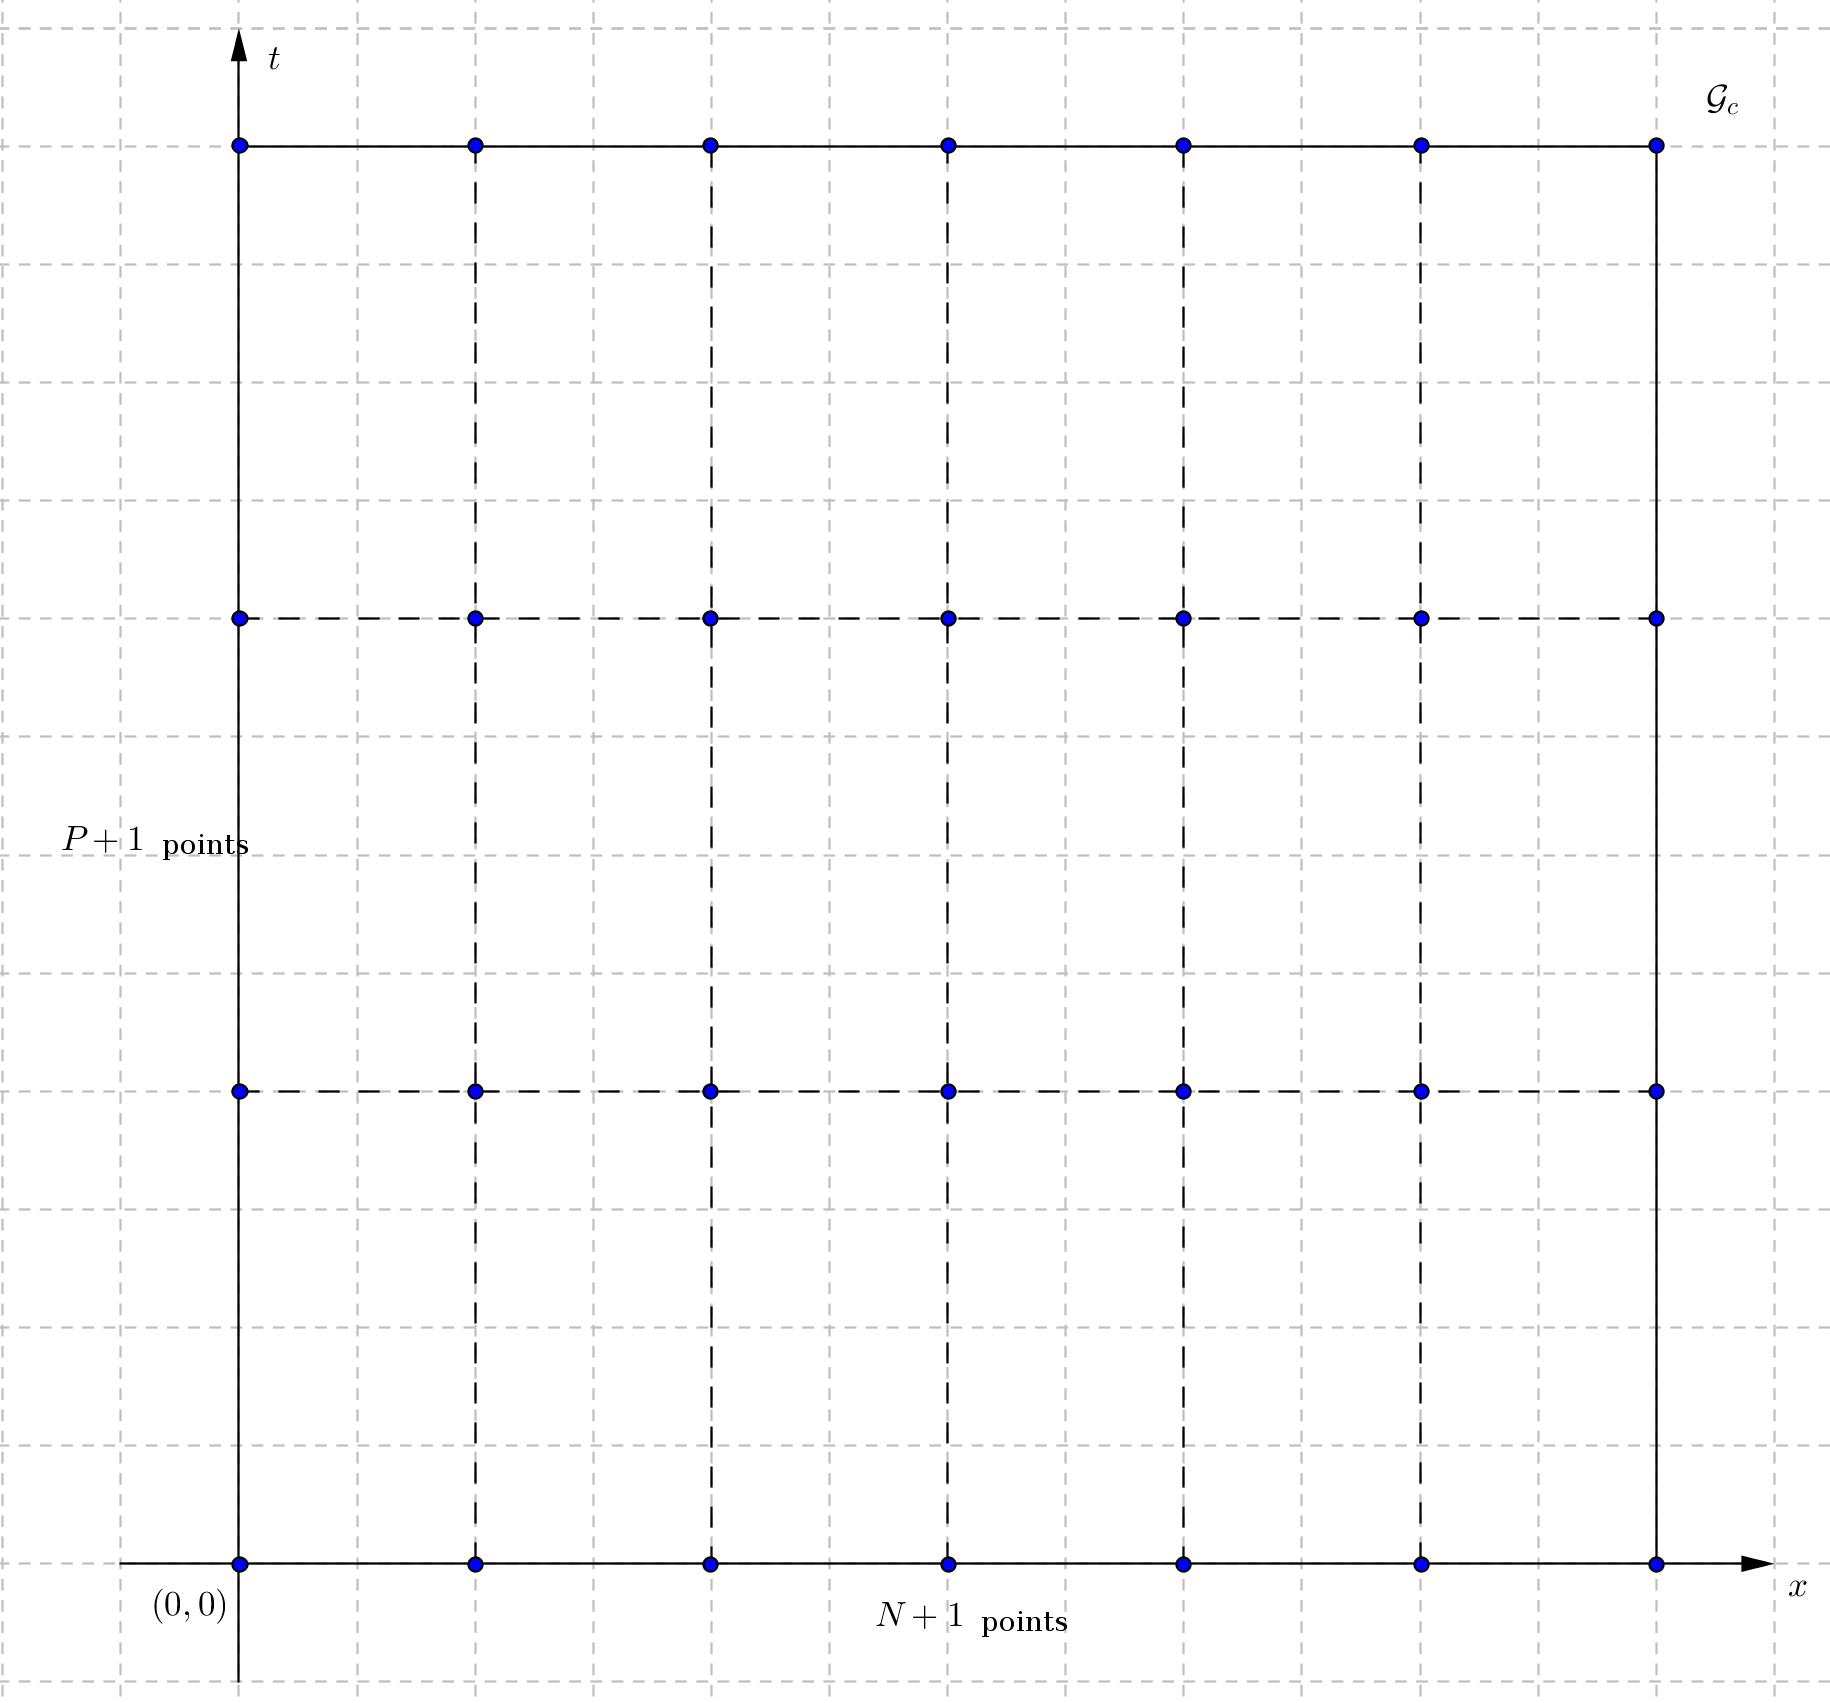
\includegraphics[width=0.9\linewidth]{img/grille_centree.png}
	\caption{Grille centrée}
	\label{fig:centered}
	\end{subfigure}
	~
	\begin{subfigure}[b]{0.3\linewidth}
	\centering
	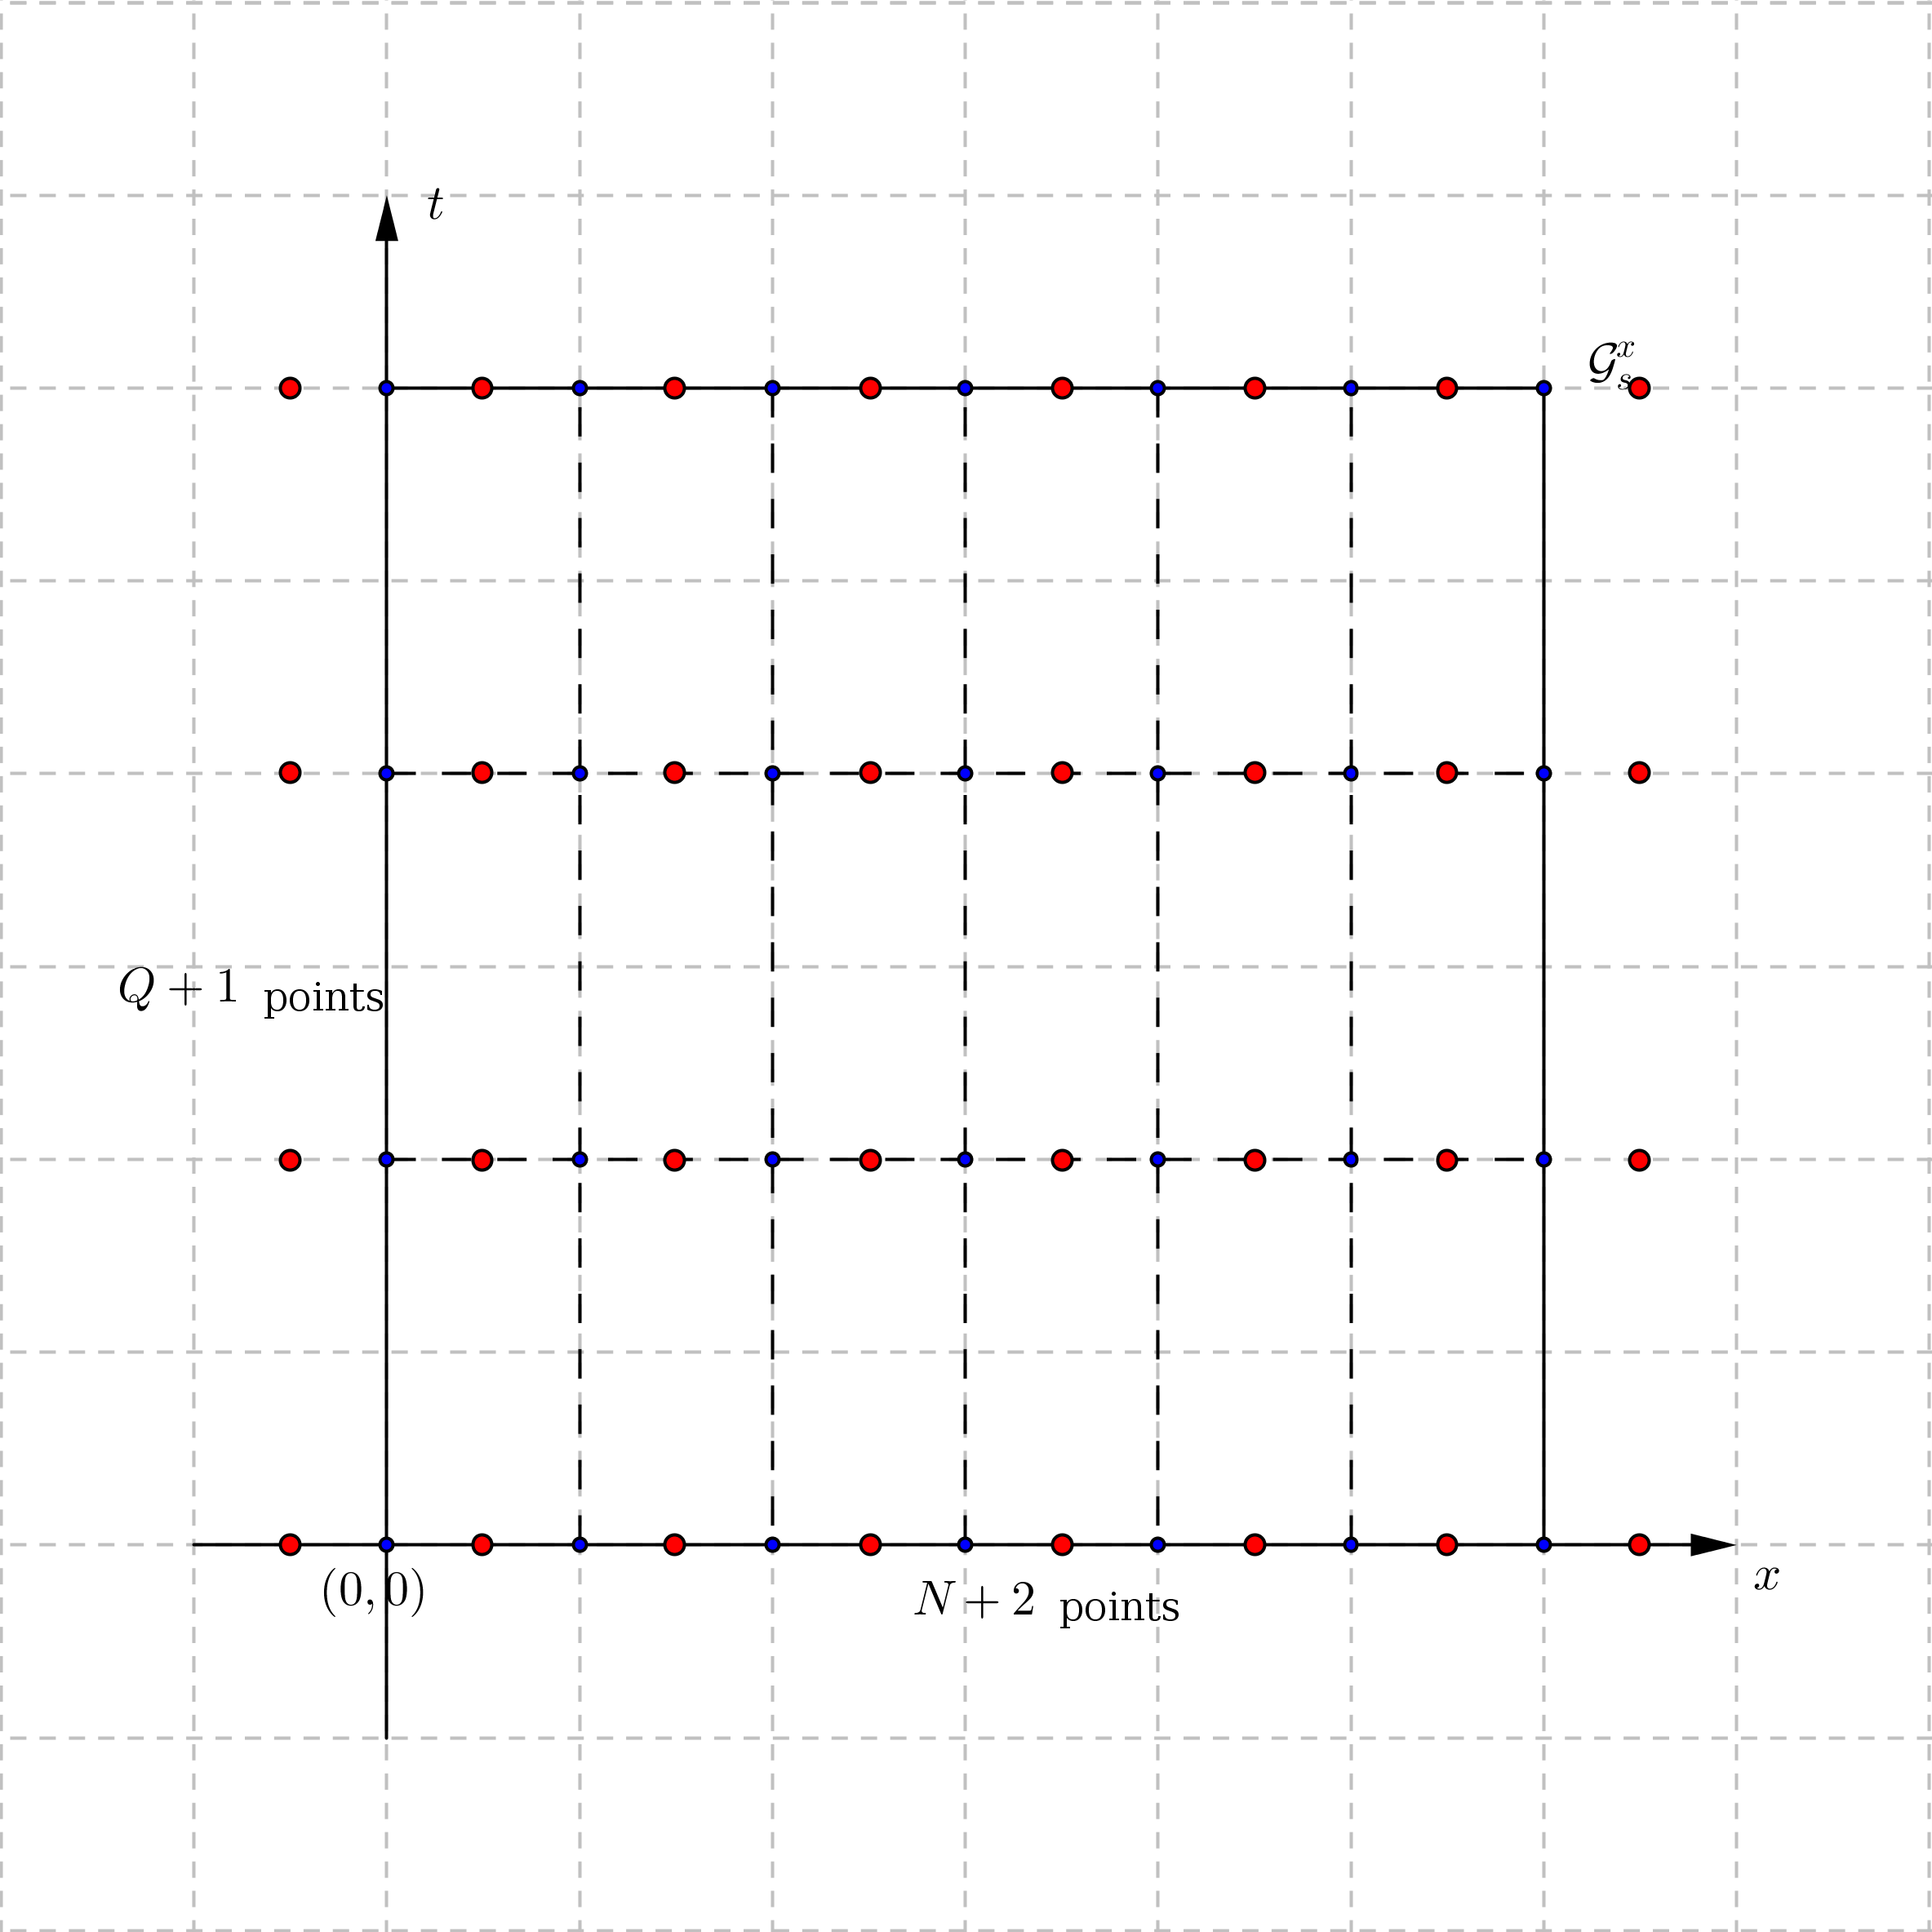
\includegraphics[width=0.9\linewidth]{img/grille_decentree_x.png}
	\caption{Grille décentrée en espace}
	\label{fig:staggeredX}
	\end{subfigure}
	~
	\begin{subfigure}[b]{0.3\linewidth}
	\centering
	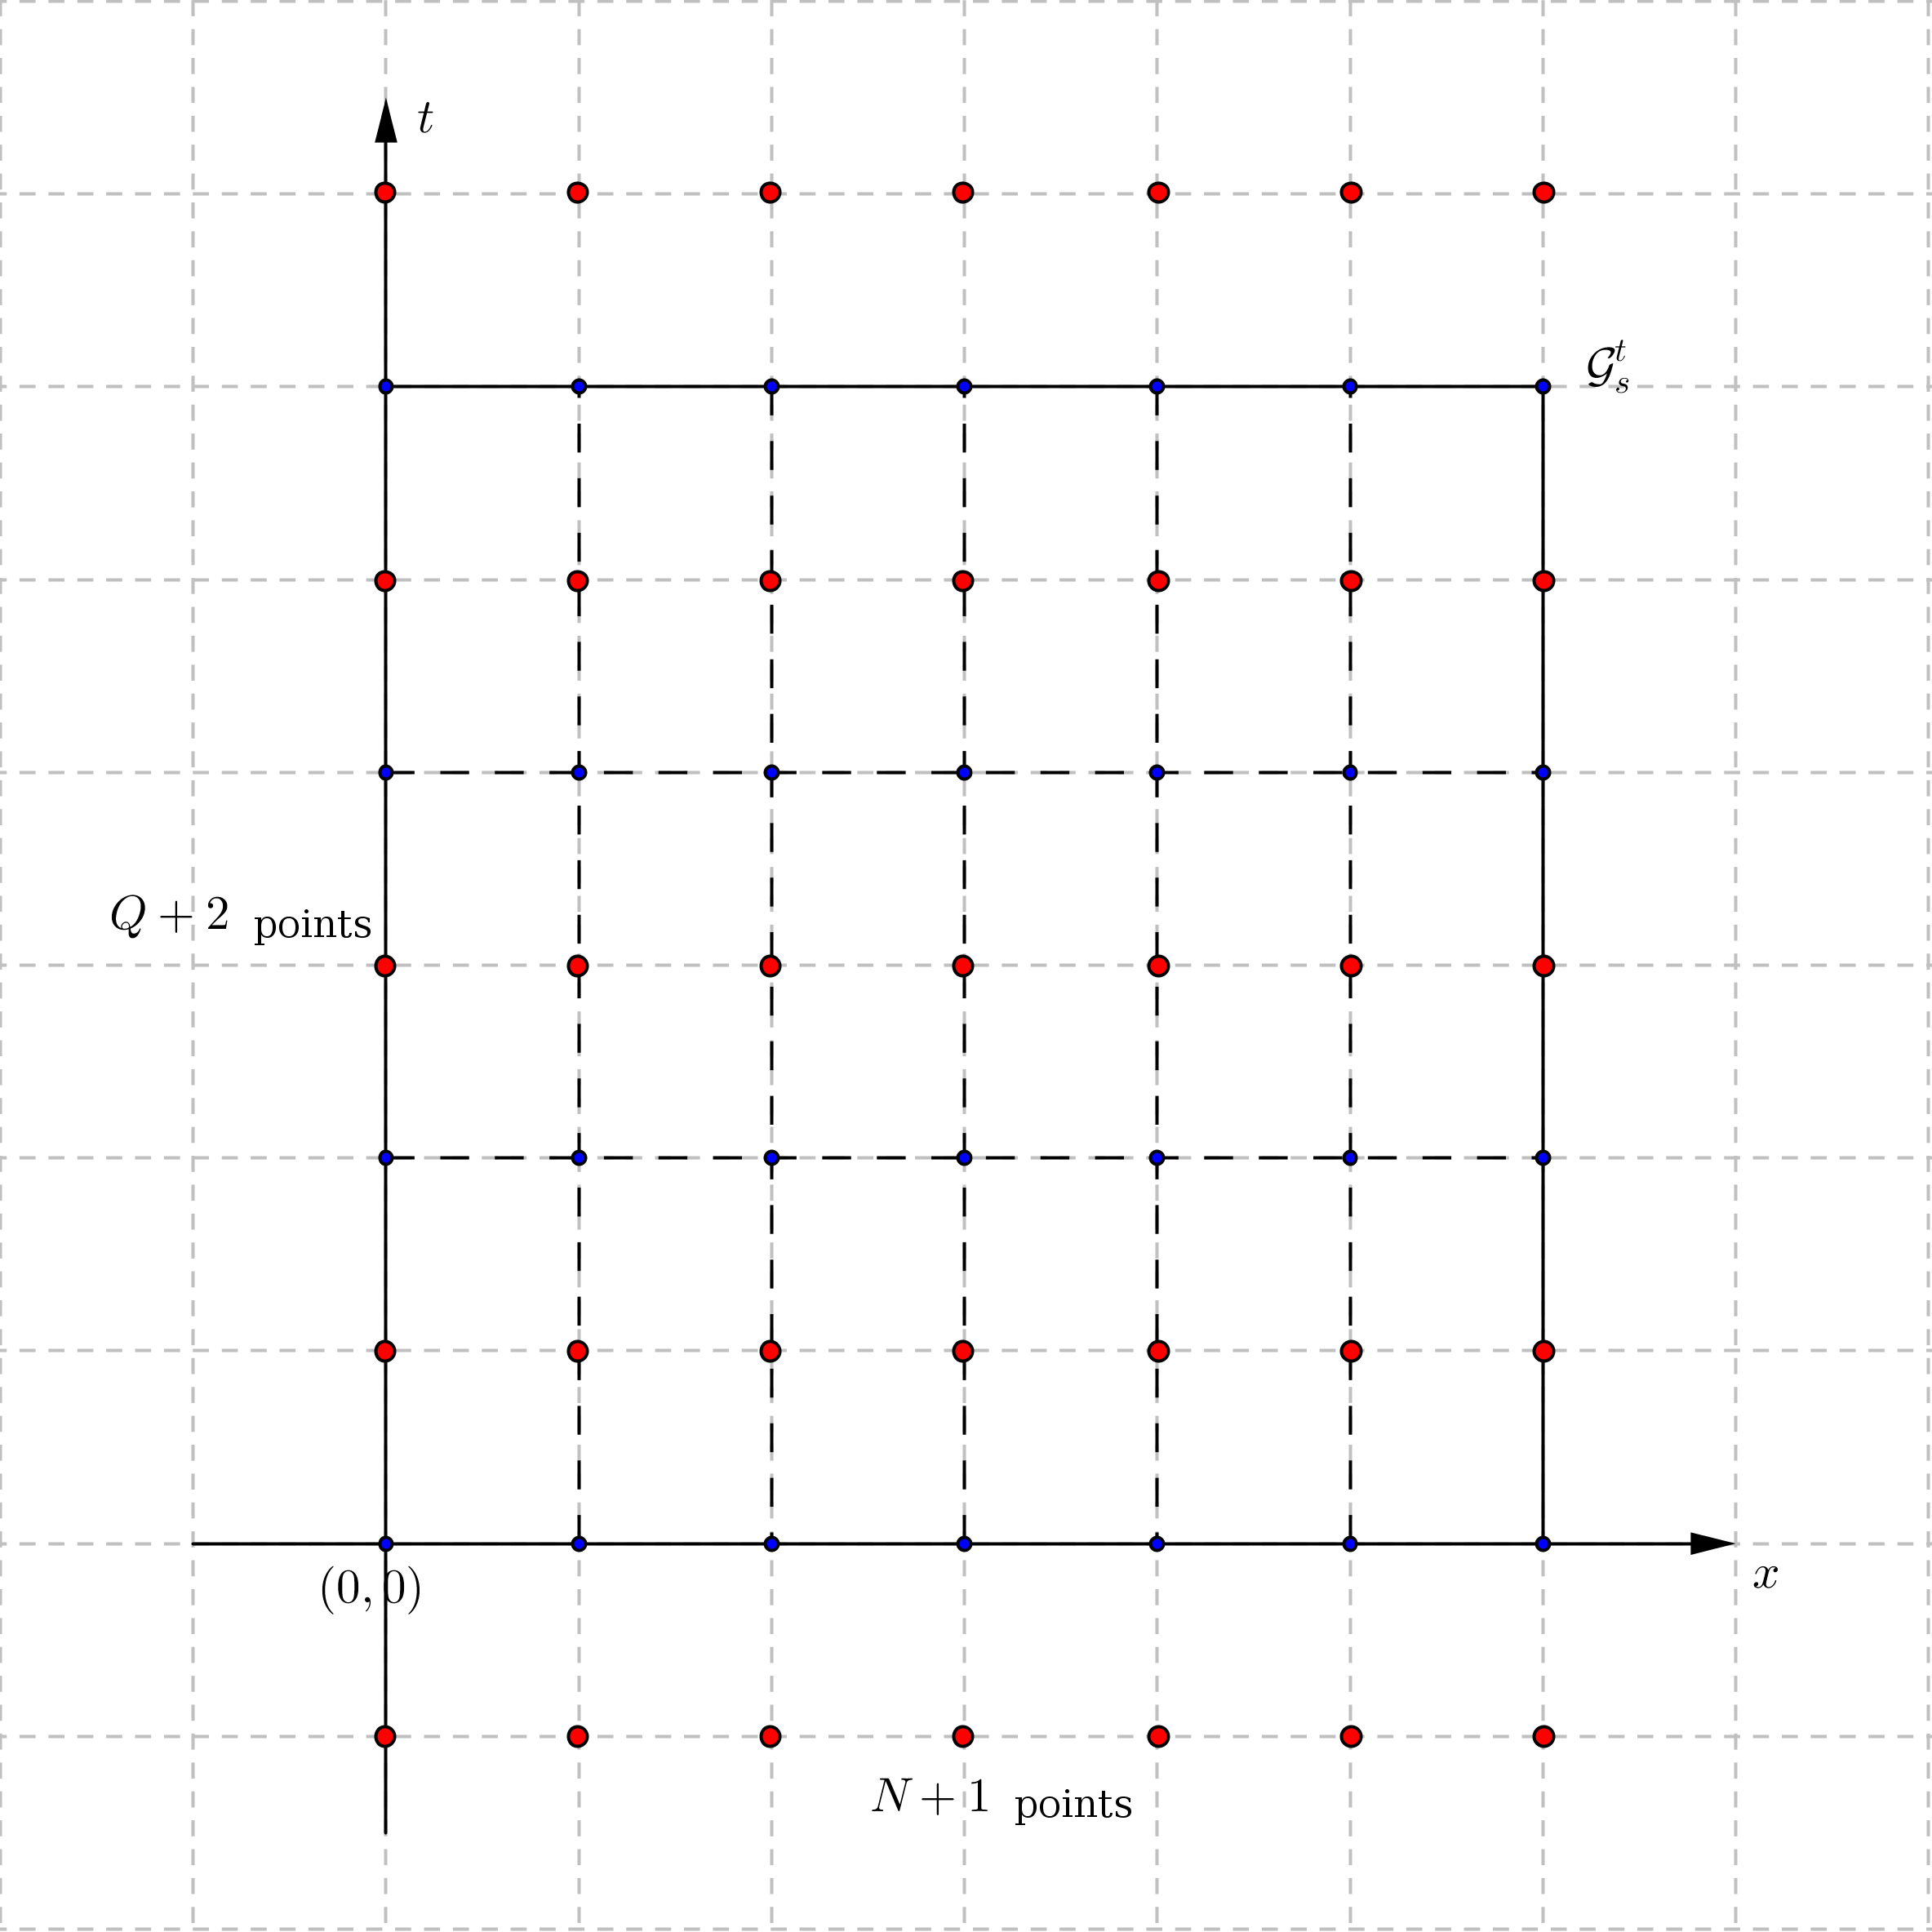
\includegraphics[width=0.9\linewidth]{img/grille_decentree_t.png}
	\caption{Grille décentrée en temps}
	\label{fig:staggeredT}
	\end{subfigure}
	\caption{Grilles de discrétisation pour $N=6$ et $Q=3$}
\end{figure}



Ainsi, $\mathbb{G}_s^x$ contient $(N+2)\times(Q+1)$ points et $\mathcal{G}_s^t$ en contient $(N+1)\times(Q+2)$ points. Notons $\mathcal{E}_s=\RR^{\mathbb{G}_s^x}\times\RR^{\mathbb{G}_s^t}$ l'espace des variables sur les grilles décentrées. Et notons 
$$
U=(\bar{m},\bar{f})=\left((\bar{m}_{ij})_{-1\leq i\leq N}^{0\leq j\leq Q}, (\bar{f}_{ij})_{0\leq i\leq N}^{-1\leq j\leq Q}\right)
$$
Les variables discrétisées. 

\subsection{Opérateurs discrétisés}
Introduisons plusieurs opérateurs, dans un premier temps, un opérateur d'interposaltion qui nous permet de lier les variables centrées aux variables décentrées. 

\begin{align}
\fonction{\mathcal{I}}{\mathcal{E}_s}{\mathcal{E}_c}{(\bar{m},\bar{f})}{\left\{
\begin{array}{ccccc}
m_{i,j} &=& (\bar{m}_{i-1,j} &+& \bar{m}_{i,j})/2 \\
f_{i,j} &=& (\bar{f}_{i,j-1} &+& \bar{f}_{i,j})/2 \\
\end{array}
\right.
\quad \forall 0\leq i\leq N,\ \forall 0\leq j\leq Q}
\end{align}

Et introduisons l'opérateur de divergence spatiale et temporelle : 
\begin{align}
\fonction{\div}{\mathcal{E}_s}{\RR^{\mathcal{G}_c}}{U}{\div(U)_{i,j} = N(\bar{m}_{i,j} - \bar{m}_{i-1,j}) + Q(\bar{f}_{i,j} - \bar{f}_{i,j-1})
}
\end{align}

Nous définissons enfin un opérateur d'extraction des frontières des variables décentrées. 

\begin{align}
\fonction{b}{\mathcal{E}_s}{\RR^{Q+1}\times\RR^{Q+1}\times\RR^{N+1}\times\RR^{N+1}}{U}{\left( (\bar{m}_{-1,j},\bar{m}_{N,j})_{j=0}^Q,(\bar{f}_{i,-1},\bar{f}_{i,Q})_{i=0}^N \right)}
\end{align}


Nous imposons les conditions aux bords suivantes :
$$
b(U) = b_0\quad b_0=(0,0,f_0,f_1)\in \RR^{Q+1}\times\RR^{Q+1}\times\RR^{N+1}\times\RR^{N+1}
$$
Avec, $f_0,\ f_1\in\RR^{N+1}$ les densités initiale et finale discrétisées en espace, et la contrainte spatiale $0\in\RR^{Q+1}$ sur la quantité de mouvement vient de la discrétisation des conditions de Neumann sur le champ de vitesse $v$. \\
Remarquons qu'en deux ou trois dimensions spatiales, les conditions de Neumann et de Dirichlet ne coïncident plus,  par exemple en 2D, les conditions de Neumann sont équivalentes à forcer la première composantes de $\bar{m}$ à être zéro sur les côtés verticaux et à forcer la seconde composante de $\bar{m}$ à être zéros sur les segments horizontaux. 

\subsection{Problème discrétisé}

Nous pouvons à présent donner le problème discrétisé, 
\begin{align}
\min_{(U,V)\in\mathcal{E}_s\times\mathcal{E}_c} \mathcal{J}(V) + \iota_{\mathcal{C}}(U) + \iota_{\mathcal{C}_s}(U,V)
\end{align}

Ici, l'indicatrice d'un ensemble convexe est définie de la façon suivante ; $ \iota_{\mathcal{C}}=\left\{\begin{array}{cl}
0 &\text{si } U\in\mathcal{C} \\
+\infty &\text{sinon }
\end{array}\right.$. Si nous notons $k=(i,j)\in\mathcal{G}_c$ les indices sur la grilles centrées, alors la fonction objectif discrète $\mathcal{J}$ s'écrit pour une variable $V\in\mathcal{E}_c$  de la manière suivante : 
$$
\mathcal{J}(V)=\sum_{k\in\mathcal{G}_c} J(m_k,f_k)
$$
Le premier ensembles de contraintes correspond à l'équation de continuité discrétisée et des conditions aux bords : 
$$
\mathcal{C}= \left\{ U\in \mathcal{E}_s\ |\ \div(U)=0,\ b(U) = b_0 \right\}
$$
Enfin, le dernier terme rajoute une contraintes liant les variables centrées et décentrées : 
$$
\mathcal{C}_s=\left\{(U,V)\in\mathcal{E}_s\times\mathcal{E}_c\ |\ V=\mathcal{I}(U)\right\}
$$


Remarquons que la fonctionnelle $\mathcal{J}$ possèdent les propriétés suivantes, lorsque que $f(t,x)\rightarrow +\infty$, $\mathcal{J}\rightarrow 0$ et que si $f(t,x)\rightarrow 0$ alors $\mathcal{J}\rightarrow +\infty$. ainsi, $\mathcal{J}$ n'est pas coercive et son gradient n'est pas lipschitzien. C'est pourquoi, les techniques de minimisation classiques (type descente de gradient) sont inefficaces et que nous allons recourir aux opérateurs proximaux et à l'algorithme de Douglas Rachford présenté dans la section précédente.  \\


Reprenons alors le problème \eqref{eq:pbmminimi} et posons, $f_1 =\mathcal{J}(V) + \iota_{\mathcal{C}}(U) $ et $f_2= \iota_{\mathcal{C}_s}(U,V)$. Ces deux fonctions sont simples dans la mesure où leur opérateur proximaux sont de la forme suivante
\begin{align}
\prox_{\gamma f_1}(U,V) & = \left(\proj_{\mathcal{C}}(U),\prox_{\gamma \mathcal{J}}(V) \right) \\
\prox_{\gamma f_2}(U,V) & = \proj_{\mathcal{C}_s}(U,V)
\end{align}
Ces opérateurs seront explicités dans la section suivante. \\
L'algorithme de Douglas-Rachford devient alors :\\

\fbox{
  \parbox{\textwidth}{
 	Soit une suite $(x_n,y_n)\in\left(\mathcal{E}_s\times\mathcal{E}_c\right)^2$. A partir, d'une condition initiale $y_0$, 
 	
 	\begin{equation}
 		\begin{aligned}
 			x_n &= \proj_{\mathcal{C}_s}(y_n) \\
 		y_{n+1} &= y_n + \lambda_n \left(\prox_{\gamma f_1}(2x_n-y_n)-x_n\right) \\
 		\end{aligned}
 	\end{equation}
 	
 	Alors $x_n\rightarrow x^{\star}$ une solution du problème. 
  }
}\\



\subsection{Opérateur proximal de $\mathcal{J}$}
La fonctionnelle $\mathcal{J}$ est simple dans le sens où son opérateur proximal peut être calculé dans une forme fermée. 
\begin{proposition}
\label{prop:proxJ}
Nous avons
\begin{align*}
\forall w\in\mathcal{G},\ \prox_{\gamma \mathcal{J}}(w) = \left( \prox_{\gamma J}(w_k)\right)_{k\in\mathcal{G}}
\end{align*}
Où, pour tout $w_k=(m_k,f_k)\in\RR^n\times\RR$, 
$$
\prox_{\gamma J}(m_k,f_k) =\left\{
\begin{array}{cl}
\left(\frac{f^{\star}_k m_k}{f^{\star}_k+\gamma} ,f^{\star}_k\right) & \text{ si } f^{\star}_k >0\\
(0,0) & \text{ sinon }
\end{array}\right.
$$
et $f^{\star}_k$ est la plus grande racine réelle du polynôme de degré 3 : 
\begin{align}
P(X) = (X-f_k)(X+\gamma)^2 -\frac{\gamma}{2}\|m_k\|^2=0
\end{align}
\end{proposition}
\begin{preuve}
Posons $(m,f)=\prox_{\gamma J}(m_k,f_k)$. Si $f>0$, comme $J$ est $C^1$ et strictement convexe sur $\RR^n\times\RR^{+,\star}$, nécessairement, $(m,f)$ est l'unique solution de $\nabla J(m,f)=0$, ce qui donne 
$$
\left\{
\begin{array}{cc}
\gamma \frac{m}{f}+m-m_k &= 0\\
-\gamma \frac{\|m\|^2}{f^2} + f-f_k &= 0
\end{array}
\right.
$$
En réarrangeant ces équations, nous obtenons bien que $P(f) = 0$ et $m=\frac{f m}{f+\gamma}$. Ce qui montre au passage que si $P$ possède au moins une racine réelle strictement positive $f^{\star}_k$, alors elle est nécessairement unique $f^{\star}_k =f $. \\
Si ce n'est pas le cas, alors nous avons nécessairement $f= 0$ et par définition de $J$, $m=0$.
\end{preuve}


\subsection{Projection sur $\mathcal{C}$}
Comme explicité dans la présentation des opérateurs proximaux, l'opérateur proximal de l'indicatrice d'un ensemble convexe et le projecteur orthogonal sur cet ensemble. Ici, l'ensemble des contraintes $\mathcal{C}$ peut être récrit comme un ensemble affine : 
\begin{align}
\mathcal{C}=\left\{U\in\mathcal{E}_s\ |\ AU=y\right\} \quad A=\begin{pmatrix}
\div \\
b
\end{pmatrix},\ y=\begin{pmatrix}
0 \\
b_0
\end{pmatrix}
\end{align}
La projection sur cet ensemble s'écrit comme un problème de minimisation strictement convexe : 
$$
\proj_{\mathcal{C}}(U) = \min_{W\in\mathcal{C}}\frac{1}{2}\|U-W\|^2
$$
Cela peut être résolu par la méthode des multiplicateurs de Lagrange. 
\begin{align*}
\text{CNS : } & \left\{ \begin{array}{rl}
W-U+A^{\star}\lambda &=0\\
AW&=y
\end{array}\right.\\
\Longleftrightarrow\quad & \left\{ \begin{array}{rl}
AW-AU+AA^{\star}\lambda &=0\\
AW&=y
\end{array}\right.\\
\Longrightarrow\quad & AA^{\star}\lambda = y-AU \\
\Longleftrightarrow\quad & \lambda = (AA^{\star})^{-1}(y-AU) \\
\Longrightarrow\quad & W = U - A^{\star} (AA^{\star})^{-1}(y-AU)
\end{align*}

Ainsi, 
\begin{align}
\proj_{\mathcal{C}}(U) = U - A^{\star} (AA^{\star})^{-1}(y-AU)
\end{align}

La question est alors de calculer efficacement l'opérateur $(AA^{\star})^{-1}$ efficacement. Cela peut être fait essentiellement de deux manières, par une méthode de gradient conjuguées qui convergera dans le pire des cas en $O(\#\mathcal{G}_s^x\times \#\mathcal{G}_s^t)$ itérations.\\

La seconde méthode est d'appliquer la transformée de Fourier pour résoudre un problème de Poisson. Nous détaillerons cette partie qui a donné beaucoup de fil à retordre lors de l'implémentation. \\

Formellent, l'équation à résoudre est la suivante : 
$$
AA^{\star} x = y-AU:= \Xi = \begin{pmatrix}
0-div(U)\\
b_0-b(U)
\end{pmatrix}
$$
où, $x$ est du même \emph{type} que $y$. Décrivons formellent ce système : 
\begin{align*}
AA^{\star}x &= \begin{bmatrix}
\div \\
b
\end{bmatrix} \begin{bmatrix}
-\nabla & b^{\star}
\end{bmatrix}
x =\Xi \\
&= \begin{bmatrix}
-\Delta & \div( b^{\star})\\
-b(\nabla) & bb^{\star} \\
\end{bmatrix}x = \Xi
\end{align*}
Remarquons que $y$ a la forme suivante, une partie qui concerne la divergence et une partie qui concerne les frontières. Prenons cette décomposition et posons, $x=\begin{pmatrix}
x_D\\x_B
\end{pmatrix}$ et $\Xi=\begin{pmatrix}
\Xi_D\\\Xi_B
\end{pmatrix}$
alors nous avons le système : 
\begin{align*}
\left\{\begin{array}{cc}
-\Delta x_D + \div(b^{\star} x_B)&=\Xi_D \\
-b(\nabla x_D) + bb^{\star} (x_B)&= \Xi_B
\end{array} 
\right. 
\end{align*}
Or, ici le choix des conditions aux bords de Neumann revèle tout son sens. En effet, nous avons alors que $b(\nabla x_D)=0$ et comme $bb^{\star}$ est l'identité sur les frontières, nous obtenons alors la solution $x_B$ explicitement. Nous avons alors à résoudre :
\begin{align*}
-\Delta x_D +  \div(b^{\star}\Xi_B) &= \Xi_D \\
-\Delta x_D  &=  \Xi_D- \div(b^{\star}\Xi_B)
\end{align*} 
C'est cette équation, munie des conditions au bords de Neumann homogène qui est résolu par la méthode de Poisson. 
En remplaçant $\Xi_D$ et $\Xi_B$ par leur valeurs, nous obtenons, le problème de poisson en fonction des données du problème : 
\begin{align}
\Delta x_D = \div(U + b^{\star}(b_0-b(U)))
\end{align}

\subsection{Projection sur $\mathcal{C}_s$}
Comme précédement, l'opérateur proximal de l'opérateur $\mathcal{C}_s$ est le projecteur orthogonal et comme précédement, nous obtenons une formule explicite à l'aide de la méthode des multiplicateurs de Lagrange. 
\begin{align}
\proj_{\mathcal{C}_s}(U,V) &= (\tilde{U},\mathcal{I}(\tilde{U}))\\
\tilde{U}&= (Id+\mathcal{I}\mathcal{I}^{\star})(U+\mathcal{I}^{\star}(V))
\end{align}


\section{Coût Généralisé}
Avant de présenter des exemple numériques, introduisons une généralisation du problème. L'outillage théorique est plus conséquent mais numériquement, les changements sont mineurs. \\
Définissons notre problème de transport discrétisé généralisé comme
\begin{align}
\min_{U\in\mathcal{E}_s}\mathcal{J}_{\omega}^{\beta}(\mathcal{I}(U))+\iota_{\mathcal{C}}(U)
\end{align}
Où, $\beta\in[0,1]$, et le vecteur de poids $\omega=(\omega_k)_{k\in\mathcal{G}_c}$ vérifie $1\leq \omega_k\leq +\infty$. La fonctionnelle généralisée est définie par : 
\begin{align}
\mathcal{J}_{\omega}^{\beta}(V) &= \sum_{k\in\mathcal{G}_c} \omega_kJ_{\beta}(m_k,f_k)\\
\forall (m,f)\in\RR\times\RR,\quad &J_{\beta}=\left\{ \begin{array}{cl}
\frac{\|m\|^2}{2f^{\beta}} & \text{si } f>0 \\
0 &\text{si } (m,f) = (0,0)\\
+\infty & \text{sinon} 
\end{array}\right.
\end{align}

Plusieurs observations, $\mathcal{J}_1^1=\mathcal{J0}$, pour tout $\beta\in [0,1]$, $\mathcal{J}_{\omega}^{\beta}$ est convexe et pour $f> 0$ nous avons 
$$
\det(\partial ^2J_{\omega}(m,f)) = \frac{\beta(1-\beta)\|m\|^2}{f^{3\beta+2}}
$$
Ainsi, $J_{\beta}$ est strictement convexe sur $\RR^n\times\RR^{+,*}$ pour $\beta \in]0,1[$. \\

\remarques{Nous pourrions expliquer que cette variante permet de généraliser le problème de transport optimal à des variétés Riemanienne. Cependant, ce qu'il faut en retenir est essentiellement 
\begin{enumerate}
\item Le coefficient $\beta\in[0,1]$ agit comme un interrupteur entre l'interpolation $L^2$ ($\beta =0$) entre les deux densités et le calcul du transport optimal ($\beta =1$), i.e. le calcul de la distance $L^2$ de Wasserstein.
\item Les poids $\omega_k$ pondèrent certaines régions de l'espace temps et permettent d'autoriser plus au moins le passage d'une densité dans une région de l'espace ; $\omega_k=+\infty$ correspond à une zone interdite. 
\end{enumerate}}

Il nous faut alors généraliser la proposition \eqref{prop:proxJ} pour le calcul de l'opérateur proximal de $\mathcal{J}_{\omega}^{\beta}$. 
\begin{proposition}
Nous avons
\begin{align*}
\forall V\in\mathcal{E}_c,\ \prox_{\gamma \mathcal{J}_{\omega}^{\beta}}(V) = \left( \prox_{\gamma\omega_k J_{\beta}}(V_k)\right)_{k\in\mathcal{G}}
\end{align*}
Où, pour tout $V_k=(m_k,f_k)\in\RR^n\times\RR$, 
$$
\prox_{\gamma J_{\beta}}(m_k,f_k) =\left\{
\begin{array}{cl}
\left(\frac{(f^{\star}_k)^{\beta} m_k}{(f^{\star}_k)^{\beta}+\gamma} ,f^{\star}_k\right) & \text{ si } f^{\star}_k >0\\
(0,0) & \text{ sinon }
\end{array}\right.
$$
et $f^{\star}_k$ est la plus grande racine réelle de l'équation en $X$ suivante : 
\begin{align}
P(X) = X ^{1-\beta}(X-f_k)(X^{\beta}+\gamma)^2 -\frac{\gamma}{2}\beta\|m_k\|^2=0
\end{align}
\end{proposition}
\begin{preuve}
C'est essentiellement la même preuve que celle de la proposition \eqref{prop:proxJ}.
\end{preuve}

\section{Exemples numériques}
Dans cette section, nous nous attacherons à démontrer l'efficacité de la méthode en montrant quelques résultats numériques. 
Les codes utilisés pour générer ces exemples sont disponibles à ce lien : \url{https://github.com/tschmoderer/transport-prj}. L'implémentation en Fortran, avec la projection sur les contraintes par la transformée en cosinus discrète est de loin la plus efficace (dossiers FFFT1D et FFFT2D). Notons ici, quelques pistes d'optimisation du code. Premièrement, la projection sur la contrainte $\mathcal{C}_s$ se fait par une descente de gradient (très rapide, 16 itérations en moyenne dans le cas 2D), cependant dans l'article de Papadakis, il est mentionné que cette projection est symétrique dans chacune des directions, et donc peut se faire en calculant explicitement l'opérateur inverse (dans une direction) une fois pour toute au début de l'algorithme et de l'appliquer ensuite directement à chaque itération dans chacune des directions. \\
Une amélioration du calcul de $\prox_{\mathcal{J}}$ est envisageable,dans la mesure où, lorsque que $\beta$ est un rationnel, cela revient à résoudre une équation polynomiale. Une autre méthode que celle de Newton Raphston pourrait aussi être utiliser (méthode de Hayley). \\
Enfin, sans doute le plus important, une recherche des paramètre $\alpha$ et $\gamma$ optimaux pourrait être envisagée. 
\newpage
\subsection{Cas 1D}
\subsubsection{Gaussiennes}
Commençons par le cas le plus simple, $f_0$ et $f_1$ sont deux gaussiennes de même variance $0.05$. Ici, le carré espace temps a été discrétisé en $N +1=100$ par $Q+1=100$ points. La paramètres sont fixés à $\alpha = 1$ et $\gamma = 1$.\\
Illustrons également la convergence de l'algorithme vers un minimum du problème, ici sur $100000$ itérations. Visualisons également le transport de la densité initiale vers la densité finale. Sans surprise, nous obtenons une ligne droite.

\begin{figure}[!h]
\centering 
	\begin{subfigure}[b]{0.48\linewidth}
	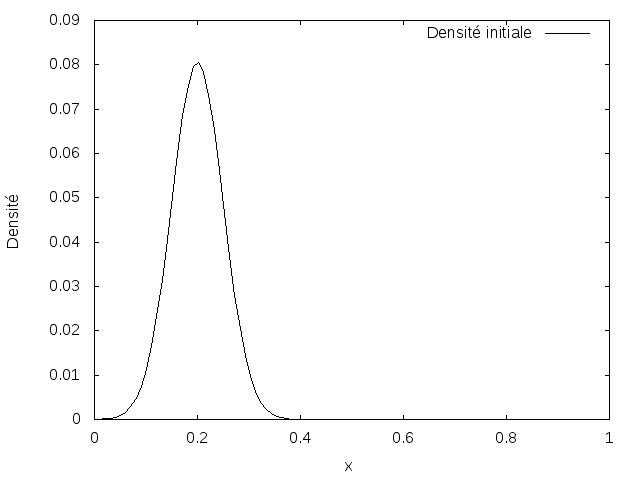
\includegraphics[width=\textwidth]{img/1DGaussian100x100/f0.png}
	\caption{Densité initiale}
	\end{subfigure}
	~
	\begin{subfigure}[b]{0.48\linewidth}
	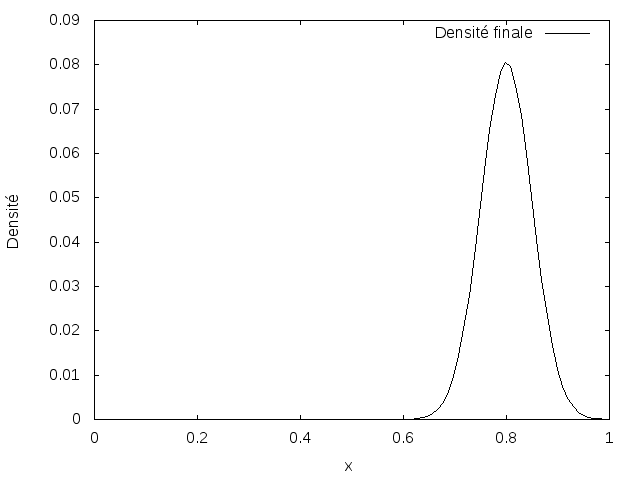
\includegraphics[width=\textwidth]{img/1DGaussian100x100/f1.png}
	\caption{Densité finale}
	\end{subfigure}
	
	\begin{subfigure}[b]{0.48\linewidth}
	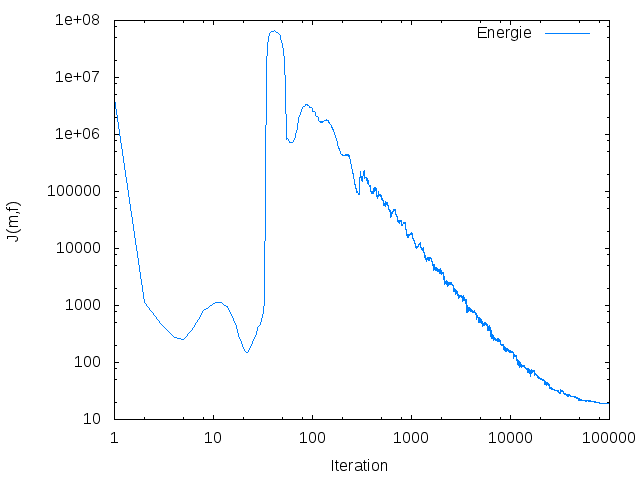
\includegraphics[width=\textwidth]{img/1DGaussian100x100/energie.png}
	\caption{$\mathcal{J}(m,f)$}
	\end{subfigure}
	~
	\begin{subfigure}[b]{0.48\linewidth}
	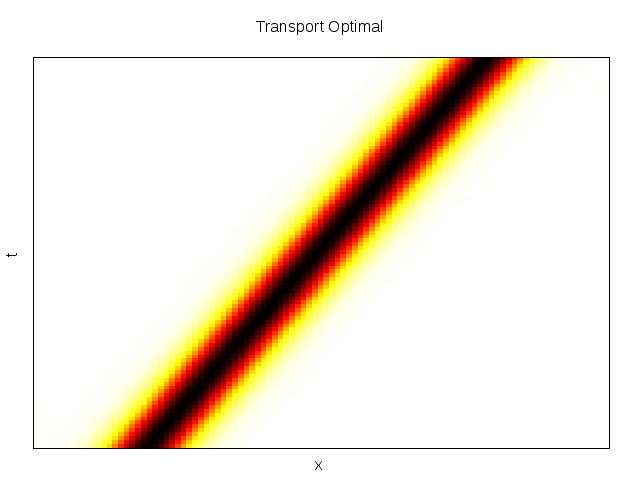
\includegraphics[width=\textwidth]{img/1DGaussian100x100/transport.png}
	\caption{Le Transport}
	\end{subfigure}	
	\caption{Données pour le transport de deux gaussiennes}
\end{figure}

\newpage
\subsubsection{Mélange de gaussiennes}
Voyons un exemple un peu plus complexe, la densité initiale est donnée par une gaussienne de variance $0.05$, la densité finale est la somme d'une gaussienne de variance $0.05$ et d'une autre gaussienne de variance $0.1$. 

\begin{figure}[!h]
\centering 
	\begin{subfigure}[b]{0.48\linewidth}
	\includegraphics[width=\textwidth]{img/1DMixture/f0.png}
	\caption{Densité initiale}
	\end{subfigure}
	~
	\begin{subfigure}[b]{0.48\linewidth}
	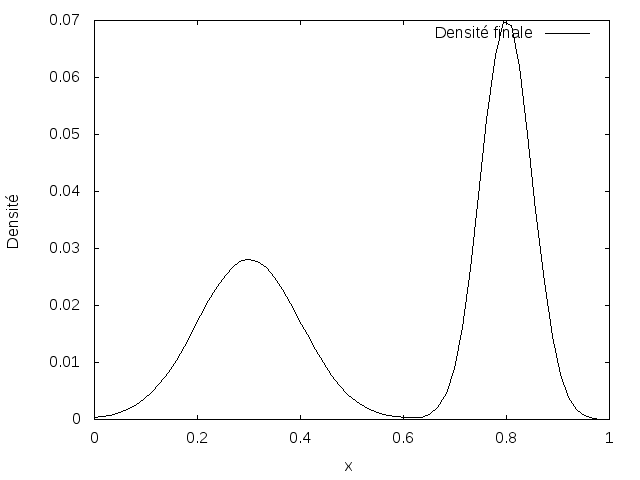
\includegraphics[width=\textwidth]{img/1DMixture/f1.png}
	\caption{Densité finale}
	\end{subfigure}
	
	\begin{subfigure}[b]{0.48\linewidth}
	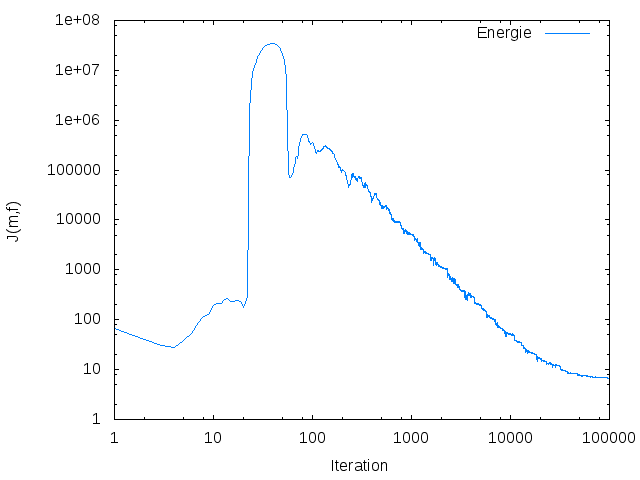
\includegraphics[width=\textwidth]{img/1DMixture/energie.png}
	\caption{$\mathcal{J}(m,f)$}
	\end{subfigure}
	~
	\begin{subfigure}[b]{0.48\linewidth}
	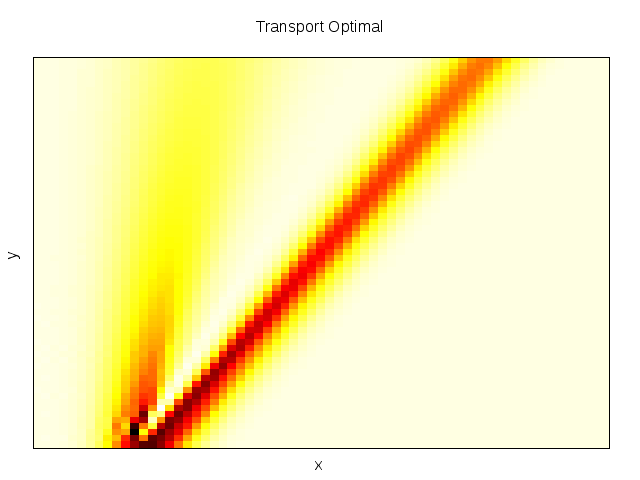
\includegraphics[width=\textwidth]{img/1DMixture/transport.png}
	\caption{Le Transport}
	\end{subfigure}	
	\caption{Données pour le transport d'une gaussienne sur deux gaussiennes}
\end{figure}

Nous voyons que l'algorithme gère bien la séparation des densités. 



\newpage


Amusons nous un peu et regardons quelques densités exotiques. 
\subsubsection{Indicatrices}
Ici, $f_0= \chi_{[0.2,0.3]}$ et $f_1=\chi_{[0.6,0.9]}$.
\begin{figure}[!h]
\centering 
	\begin{subfigure}[b]{0.48\linewidth}
	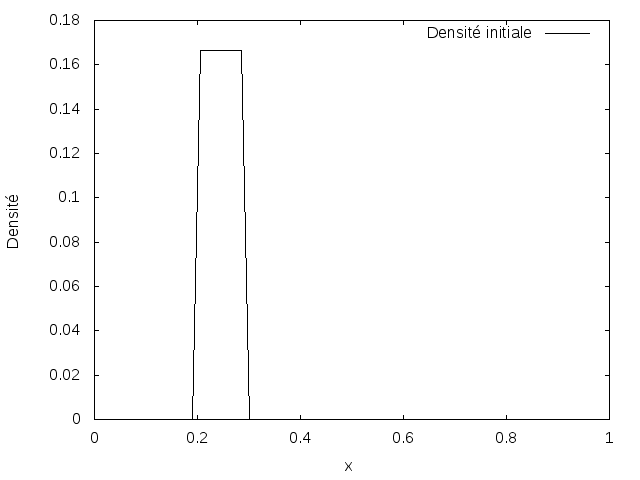
\includegraphics[width=\textwidth]{img/1DIndicatrix/f0.png}
	\caption{Densité initiale}
	\end{subfigure}
	~
	\begin{subfigure}[b]{0.48\linewidth}
	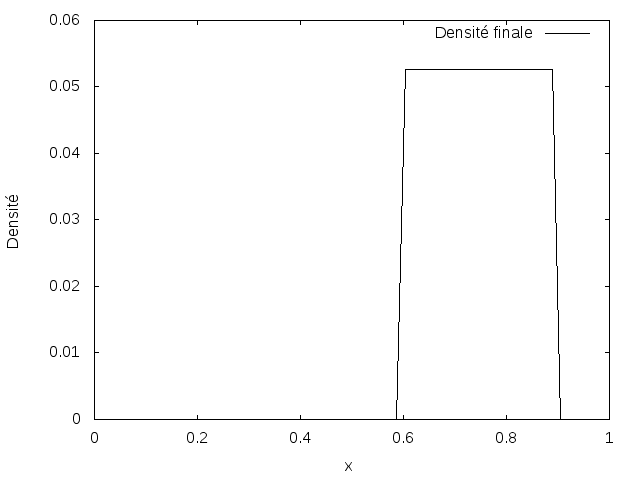
\includegraphics[width=\textwidth]{img/1DIndicatrix/f1.png}
	\caption{Densité finale}
	\end{subfigure}
	
	\begin{subfigure}[b]{0.48\linewidth}
	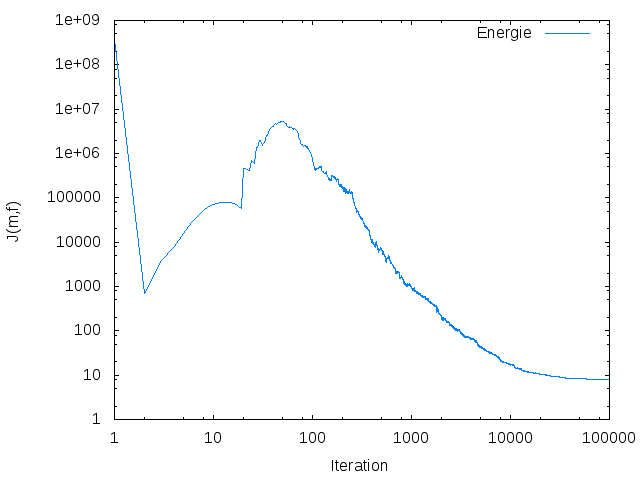
\includegraphics[width=\textwidth]{img/1DIndicatrix/energie.png}
	\caption{$\mathcal{J}(m,f)$}
	\end{subfigure}
	~
	\begin{subfigure}[b]{0.48\linewidth}
	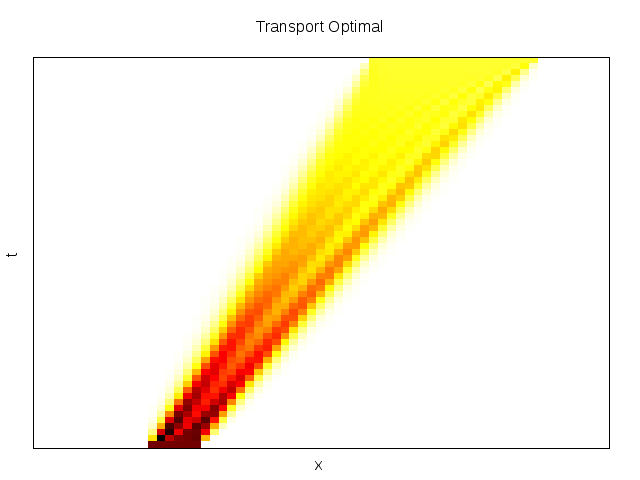
\includegraphics[width=\textwidth]{img/1DIndicatrix/transport.png}
	\caption{Le Transport}
	\end{subfigure}	
	\caption{Données pour le transport d'indicatrices}
\end{figure}
\newpage


\subsubsection{Coût généralisé}
Reprenons nos deux braves gaussiennes du premier exemple, et regardons l'effet du paramètre $\beta$ sur le transport. 
\begin{figure}[!h]
\centering 
%	\begin{subfigure}[b]{0.48\linewidth}
%	\includegraphics[width=\textwidth]{img/1DGeneralise/f0.png}
%	\caption{Densité initiale}
%	\end{subfigure}
%	~
%	\begin{subfigure}[b]{0.48\linewidth}
%	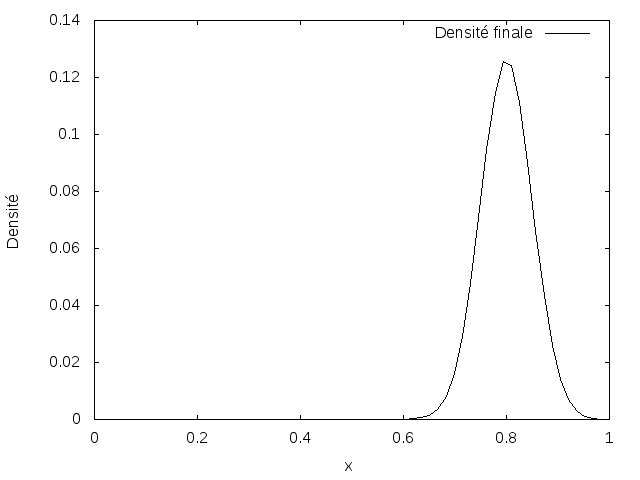
\includegraphics[width=\textwidth]{img/1DGeneralise/f1.png}
%	\caption{Densité finale}
%	\end{subfigure}
	
	\begin{subfigure}[b]{0.48\linewidth}
	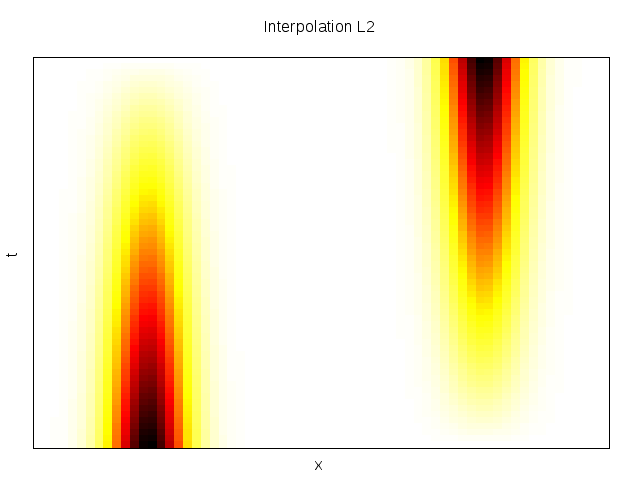
\includegraphics[width=\textwidth]{img/1DGeneralise/transport0.png}
	\caption{$\beta = 0$}
	\end{subfigure}
	~
	\begin{subfigure}[b]{0.48\linewidth}
	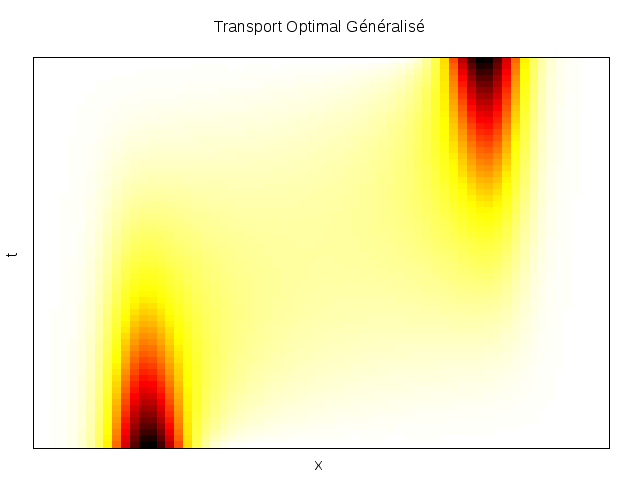
\includegraphics[width=\textwidth]{img/1DGeneralise/transport25.png}
	\caption{$\beta = 1/4$}
	\end{subfigure}	
	
	\begin{subfigure}[b]{0.48\linewidth}
	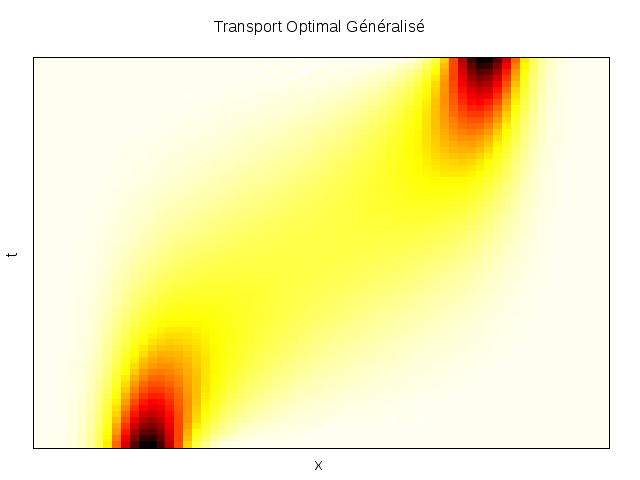
\includegraphics[width=\textwidth]{img/1DGeneralise/transport50.png}
	\caption{$\beta = 1/2$}
	\end{subfigure}
	~
	\begin{subfigure}[b]{0.48\linewidth}
	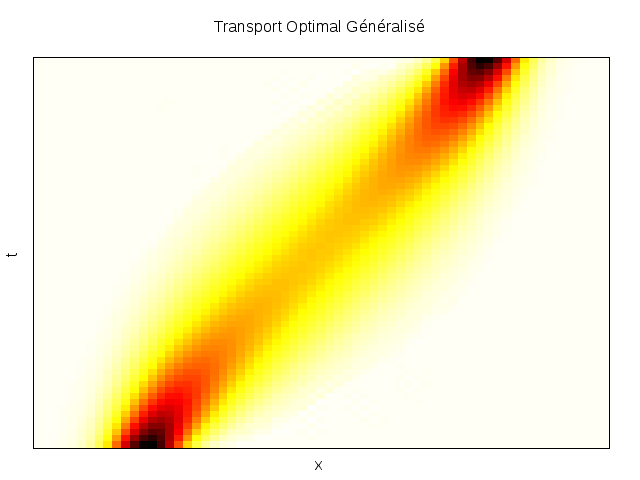
\includegraphics[width=\textwidth]{img/1DGeneralise/transport75.png}
	\caption{$\beta = 3/4$}
	\end{subfigure}	
	
	\begin{subfigure}[b]{0.48\linewidth}
	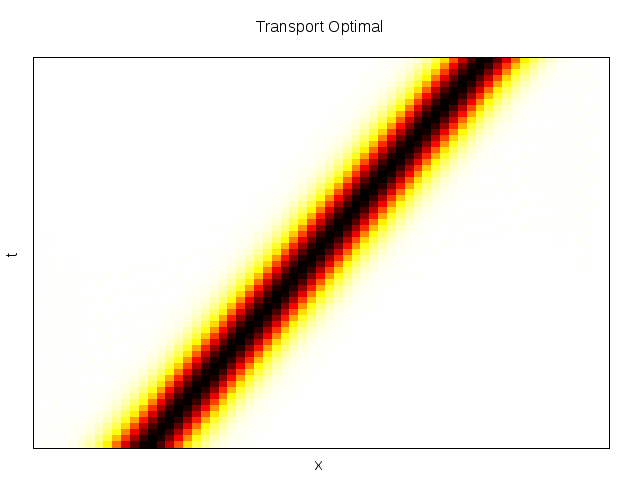
\includegraphics[width=\textwidth]{img/1DGeneralise/transport100.png}
	\caption{$\beta = 1$}
	\end{subfigure}	
	\caption{Les transports de deux gaussiennes pour différentes valeurs de $\beta$}
\end{figure}

Comme nous l'avions annoncé, l' paramètre $\beta$ agit comme un interrupteur entre l'interpolation $L^2$ et l'application de transport; Plus $\beta$ se rapproche de $1$ plus on se rapproche de l'application de transport optimal. 

\newpage
\subsubsection{Obstacle}

Une autre caractéristique que nous pouvons faire varier est la présence d'obstacles sur le parcours. Prenons deux braves gaussiennes centrées spatialement et de même variance $0.05$ et mettons un obstacle en plein milieu du passage. 

\begin{figure}[!h]
\centering 
	\begin{subfigure}[b]{0.48\linewidth}
	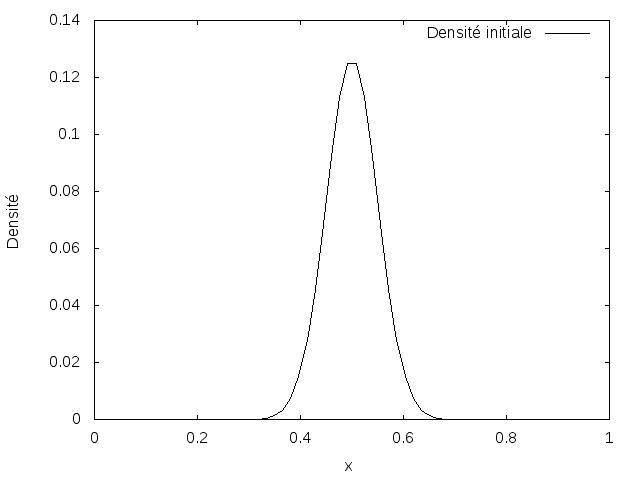
\includegraphics[width=\textwidth]{img/1DObstacle/f0.png}
	\caption{Densité initiale}
	\end{subfigure}
	~
	\begin{subfigure}[b]{0.48\linewidth}
	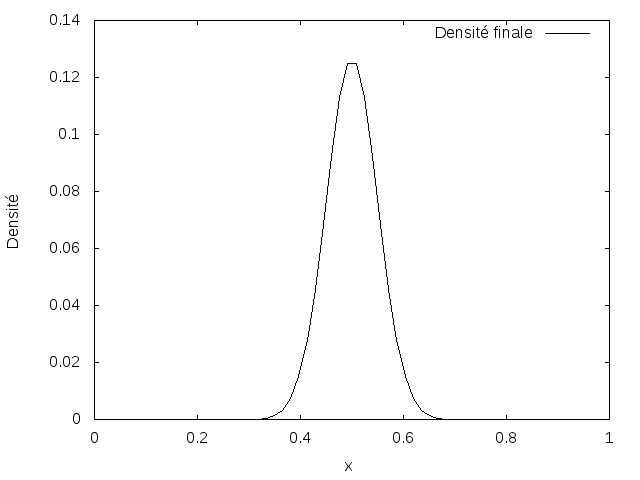
\includegraphics[width=\textwidth]{img/1DObstacle/f1.png}
	\caption{Densité finale}
	\end{subfigure}
	
	\begin{subfigure}[b]{0.48\linewidth}
	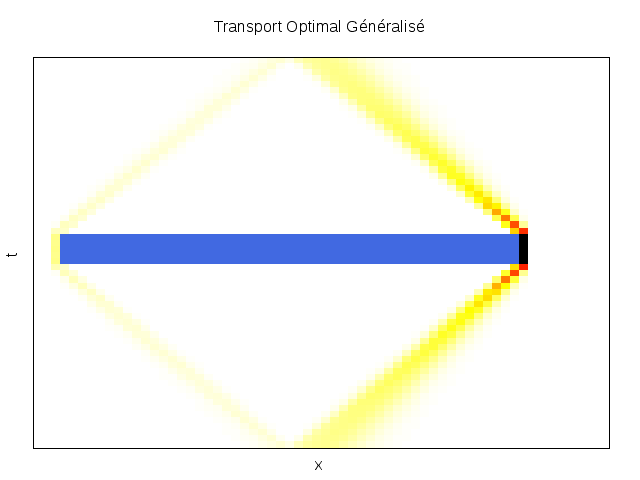
\includegraphics[width=\textwidth]{img/1DObstacle/resultat.png}
	\caption{Un obstacle au milieu du passage}
	\end{subfigure}
	~
	\begin{subfigure}[b]{0.48\linewidth}
	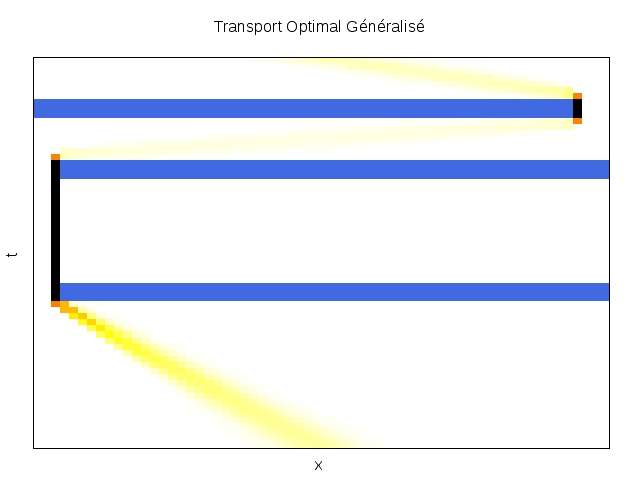
\includegraphics[width=\textwidth]{img/1DLabyrinthe/resultat.png}
	\caption{Un "labyrinthe"}
	\end{subfigure}	
	\caption{Transport de deux gaussiennes avec des obstacles}
\end{figure}

\newpage




\newpage
\subsection{Cas 2D}
L'extension du code en deux dimensions spatiales est immédiate. 
\subsubsection{Gaussiennes}
Prenons deux gaussiennes de même variance 
\begin{figure}[!h]
\centering 
\hspace{-0.5cm}
	\begin{subfigure}[b]{0.3\linewidth}
	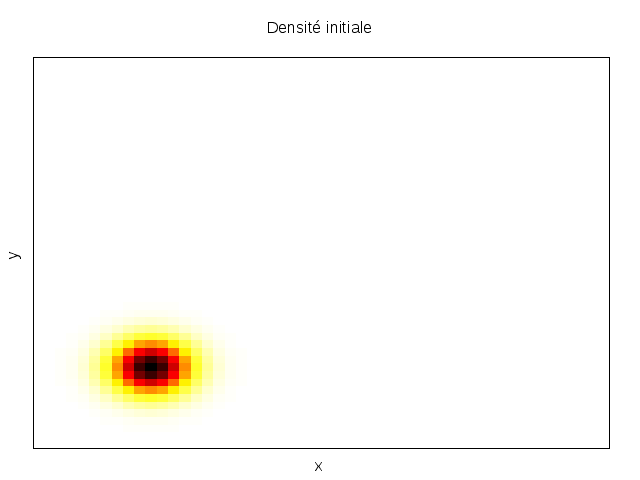
\includegraphics[width=\textwidth]{img/2DGaussian/f0.png}
	\caption{Densité initiale}
	\end{subfigure}
	~
	\begin{subfigure}[b]{0.3\linewidth}
	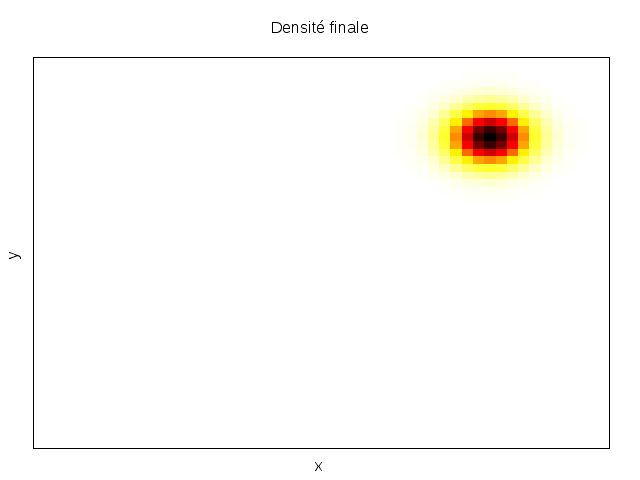
\includegraphics[width=\textwidth]{img/2DGaussian/f1.png}
	\caption{Densité finale}
	\end{subfigure}
	~
	\begin{subfigure}[b]{0.35\linewidth}
	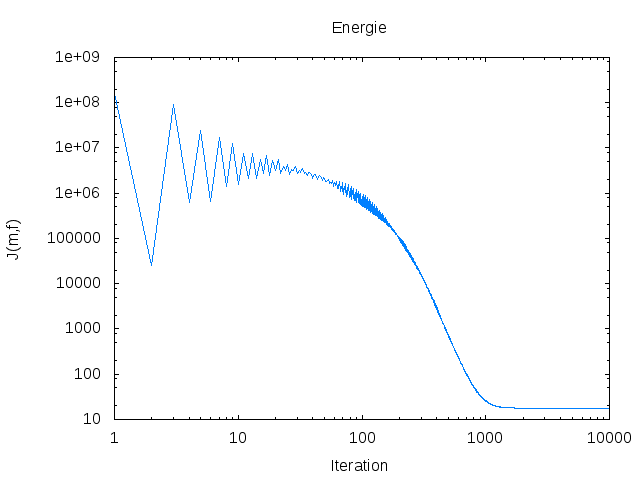
\includegraphics[width=\textwidth]{img/2DGaussian/energie.png}
	\caption{Energie}
	\end{subfigure}
	~
	
	\begin{subfigure}[b]{0.22\linewidth}
	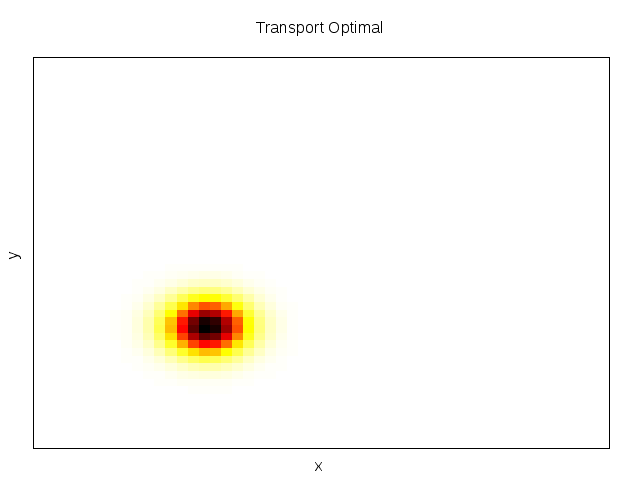
\includegraphics[width=\textwidth]{img/2DGaussian/C_00010.png}
	\caption{$t=0.2$}
	\end{subfigure}
	~
	\begin{subfigure}[b]{0.22\linewidth}
	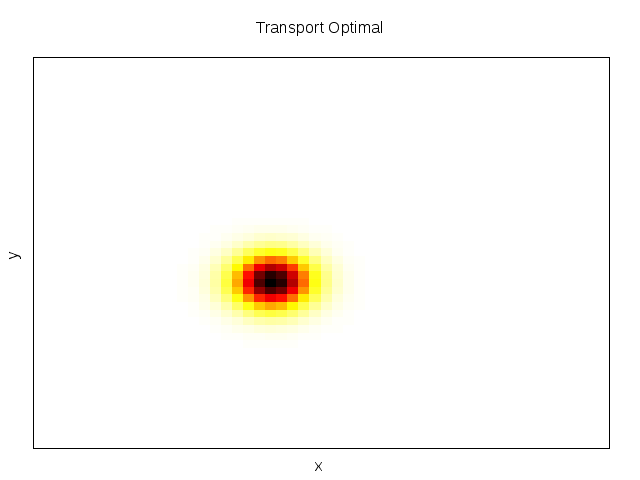
\includegraphics[width=\textwidth]{img/2DGaussian/C_00020.png}
	\caption{$t=0.4$}
	\end{subfigure}
	~
	\begin{subfigure}[b]{0.22\linewidth}
	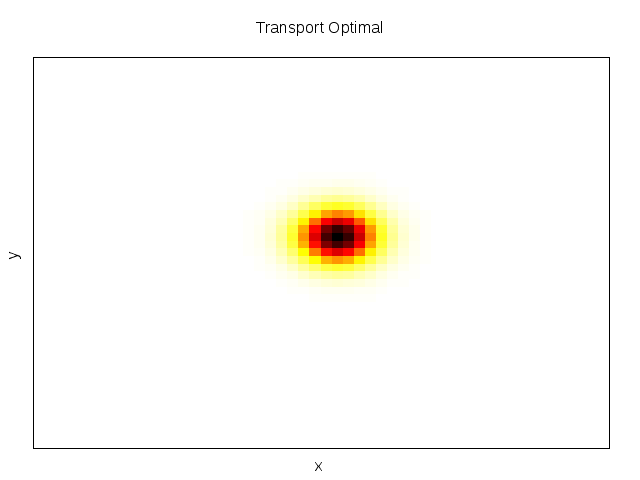
\includegraphics[width=\textwidth]{img/2DGaussian/C_00030.png}
	\caption{$t=0.6$}
	\end{subfigure}
	~
	\begin{subfigure}[b]{0.22\linewidth}
	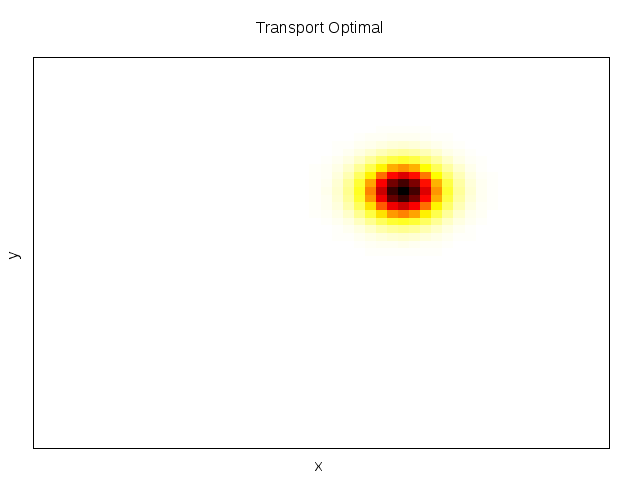
\includegraphics[width=\textwidth]{img/2DGaussian/C_00040.png}
	\caption{$t=0.8$}
	\end{subfigure}
	\caption{Transport de deux gaussiennes $N=P=Q=50$}
\end{figure}

Encore une fois, le transport optimal déterminé est une ligne droite, c'est cohérent avec ce que nous savons. Voyons comment l'algorithme se comporte avec une combinaison de gaussiennes. Partons de la même gaussienne que précédemment et prenons comme densité d'arrivé deux gaussiennes de variances différentes. 

\begin{figure}[!h]
\vspace{-0.5cm}
\centering 
\hspace{-0.5cm}
	\begin{subfigure}[b]{0.3\linewidth}
	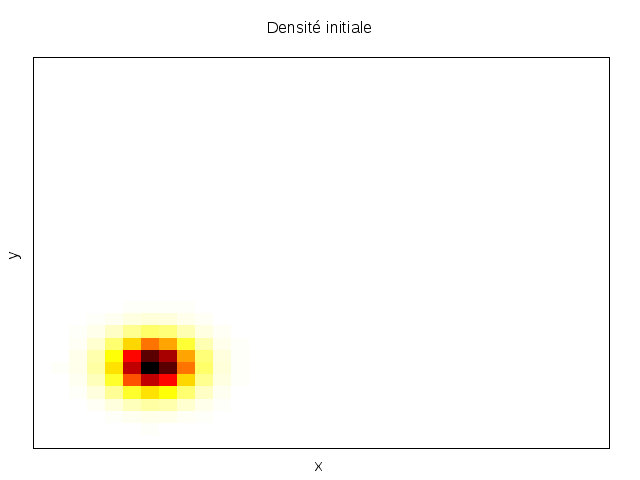
\includegraphics[width=\textwidth]{img/2DMixture/f0.png}
	\caption{Densité initiale}
	\end{subfigure}
	~
	\begin{subfigure}[b]{0.3\linewidth}
	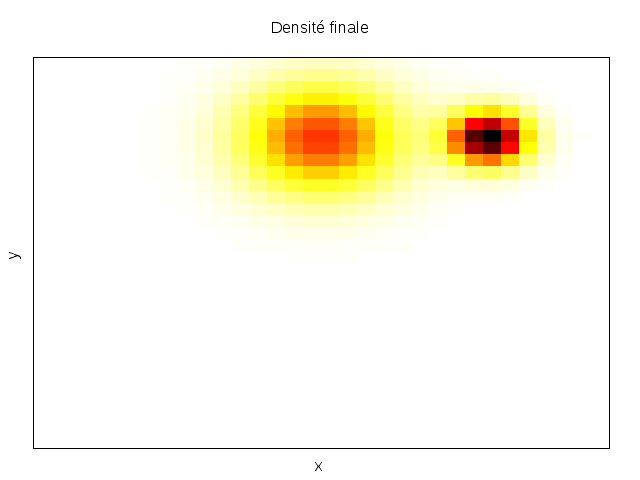
\includegraphics[width=\textwidth]{img/2DMixture/f1.png}
	\caption{Densité finale}
	\end{subfigure}
	~
	\begin{subfigure}[b]{0.35\linewidth}
	\includegraphics[width=\textwidth]{img/2DMixture/energie.png}
	\caption{Energie}
	\end{subfigure}
	~
	
	\begin{subfigure}[b]{0.22\linewidth}
	\includegraphics[width=\textwidth]{img/2DMixture/C_00007.png}
	\caption{$t=0.2$}
	\end{subfigure}
	~
	\begin{subfigure}[b]{0.22\linewidth}
	\includegraphics[width=\textwidth]{img/2DMixture/C_00014.png}
	\caption{$t=0.4$}
	\end{subfigure}
	~
	\begin{subfigure}[b]{0.22\linewidth}
	\includegraphics[width=\textwidth]{img/2DMixture/C_00021.png}
	\caption{$t=0.6$}
	\end{subfigure}
	~
	\begin{subfigure}[b]{0.22\linewidth}
	\includegraphics[width=\textwidth]{img/2DMixture/C_00028.png}
	\caption{$t=0.8$}
	\end{subfigure}
	\caption{Transport de deux gaussiennes $N=P=Q=31$}
\end{figure}





\newpage


\subsubsection{Coût généralisé}
Comme nous l'avions fait précédemment, faisons varier le paramètre $_beta$. Nous observons une fois encore que plus $_beta$ est proche de $1$, plus on est proche de l'application de transport optimal, plus on est proche de $0$, plus on se rapproche de l'interpolation $L^2$. \\

\begin{figure}[!h]
\centering
\begin{tabular}{ccccccc}
\rotatebox[origin=p]{90}{$\quad\qquad\ \beta = 0$} & 
\includegraphics[width=0.15\linewidth]{img/2DGeneralise/f0.png} & 
\includegraphics[width=0.15\linewidth]{img/2DGeneralise/0_C_00007.png} & \includegraphics[width=0.15\linewidth]{img/2DGeneralise/0_C_00014.png} & \includegraphics[width=0.15\linewidth]{img/2DGeneralise/0_C_00021.png} & \includegraphics[width=0.15\linewidth]{img/2DGeneralise/0_C_00028.png} & \includegraphics[width=0.15\linewidth]{img/2DGeneralise/f1.png} \\ [-20pt]

\rotatebox[origin=c]{90}{$\quad\qquad\ \beta = 0.25$} &
\includegraphics[width=0.15\linewidth]{img/2DGeneralise/f0.png} & 
\includegraphics[width=0.15\linewidth]{img/2DGeneralise/25_C_00007.png} & \includegraphics[width=0.15\linewidth]{img/2DGeneralise/25_C_00014.png} & \includegraphics[width=0.15\linewidth]{img/2DGeneralise/25_C_00021.png} & \includegraphics[width=0.15\linewidth]{img/2DGeneralise/25_C_00028.png} & \includegraphics[width=0.15\linewidth]{img/2DGeneralise/f1.png} \\ [-20pt]

\rotatebox[origin=c]{90}{$\quad\qquad\ \beta = 0.5$} &
\includegraphics[width=0.15\linewidth]{img/2DGeneralise/f0.png} & 
\includegraphics[width=0.15\linewidth]{img/2DGeneralise/50_C_00007.png} & \includegraphics[width=0.15\linewidth]{img/2DGeneralise/50_C_00014.png} & \includegraphics[width=0.15\linewidth]{img/2DGeneralise/50_C_00021.png} & \includegraphics[width=0.15\linewidth]{img/2DGeneralise/50_C_00028.png} & \includegraphics[width=0.15\linewidth]{img/2DGeneralise/f1.png} \\ [-20pt]

\rotatebox[origin=c]{90}{$\quad\qquad\ \beta = 0.75$} &
\includegraphics[width=0.15\linewidth]{img/2DGeneralise/f0.png} & 
\includegraphics[width=0.15\linewidth]{img/2DGeneralise/75_C_00007.png} & \includegraphics[width=0.15\linewidth]{img/2DGeneralise/75_C_00014.png} & \includegraphics[width=0.15\linewidth]{img/2DGeneralise/75_C_00021.png} & \includegraphics[width=0.15\linewidth]{img/2DGeneralise/75_C_00028.png} & \includegraphics[width=0.15\linewidth]{img/2DGeneralise/f1.png} \\ [-20pt]

\rotatebox[origin=c]{90}{$\quad\qquad\ \beta = 1$} &
\includegraphics[width=0.15\linewidth]{img/2DGeneralise/f0.png} & 
\includegraphics[width=0.15\linewidth]{img/2DGeneralise/100_C_00007.png} & \includegraphics[width=0.15\linewidth]{img/2DGeneralise/100_C_00014.png} & \includegraphics[width=0.15\linewidth]{img/2DGeneralise/100_C_00021.png} & \includegraphics[width=0.15\linewidth]{img/2DGeneralise/100_C_00028.png} & \includegraphics[width=0.15\linewidth]{img/2DGeneralise/f1.png} \\ [-20pt]

& $t=0$ & $t=0.2$ & $t=0.4$ & $t=0.6$ & $t=0.8$ & $t=1$ \\
\end{tabular}
\caption{Évolution de $f^{\star}(\cdot,t)$ pour différentes valeurs de $\beta$ et $t$. La première et la dernière image de chaque ligne sont les densités initiale et finale}
\end{figure}




\newpage
\subsubsection{Labyrinthe}
Amusons nous à mettre des obstacles sur le passage de la densité, prenons deux gaussiennes centrées sur le domaine et de variance $0.01$.\\

\begin{figure}[!h]
\centering
\begin{subfigure}[b]{0.45\linewidth}
\includegraphics[width=\linewidth]{img/2DObstacle/f0.png}
\caption{Densité initiale}
\end{subfigure}
~
\begin{subfigure}[b]{0.45\linewidth}
\includegraphics[width=\linewidth]{img/2DObstacle/f1.png}
\caption{Densité finale}
\end{subfigure}

\begin{subfigure}[b]{0.18\linewidth}
\includegraphics[width=\linewidth]{img/2DObstacle/T_00007.png}
\caption{$t=0.2$}
\end{subfigure}
~
\begin{subfigure}[b]{0.18\linewidth}
\includegraphics[width=\linewidth]{img/2DObstacle/T_00014.png}
\caption{$t=0.45$}
\end{subfigure}
~
\begin{subfigure}[b]{0.18\linewidth}
\includegraphics[width=\linewidth]{img/2DObstacle/T_00018.png}
\caption{$t=0.55$}
\end{subfigure}
~
\begin{subfigure}[b]{0.18\linewidth}
\includegraphics[width=\linewidth]{img/2DObstacle/T_00021.png}
\caption{$t=0.6$}
\end{subfigure}
~
\begin{subfigure}[b]{0.18\linewidth}
\includegraphics[width=\linewidth]{img/2DObstacle/T_00028.png}
\caption{$t=0.8$}
\end{subfigure}

\caption{Transport de deux gaussiennes avec un obstacle pour $t\in[0.45,0.55]$}
\end{figure}

Passons à un de mes exemples préférés, celui où l'obstacle est un labyrinthe. En entrant les densités initiale et finale, le transport se déplacera dans le labyrinthe en suivant le chemin le plus court. 

\begin{figure}[!h]
\centering
\begin{subfigure}[b]{0.23\linewidth}
\includegraphics[width=\linewidth]{img/2DLabyrinthe/T_00001.png}
\caption*{$t=0$}
\end{subfigure}
~
\begin{subfigure}[b]{0.23\linewidth}
\includegraphics[width=\linewidth]{img/2DLabyrinthe/T_00006.png}
\caption*{$t=0.05$}
\end{subfigure}
~
\begin{subfigure}[b]{0.23\linewidth}
\includegraphics[width=\linewidth]{img/2DLabyrinthe/T_00012.png}
\caption*{$t=0.11$}
\end{subfigure}
~
\begin{subfigure}[b]{0.23\linewidth}
\includegraphics[width=\linewidth]{img/2DLabyrinthe/T_00017.png}
\caption*{$t=0.16$}
\end{subfigure}

\begin{subfigure}[b]{0.23\linewidth}
\includegraphics[width=\linewidth]{img/2DLabyrinthe/T_00023.png}
\caption*{$t=0.22$}
\end{subfigure}
~
\begin{subfigure}[b]{0.23\linewidth}
\includegraphics[width=\linewidth]{img/2DLabyrinthe/T_00028.png}
\caption*{$t=0.27$}
\end{subfigure}
~
\begin{subfigure}[b]{0.23\linewidth}
\includegraphics[width=\linewidth]{img/2DLabyrinthe/T_00034.png}
\caption*{$t=0.33$}
\end{subfigure}
~
\begin{subfigure}[b]{0.23\linewidth}
\includegraphics[width=\linewidth]{img/2DLabyrinthe/T_00039.png}
\caption*{$t=0.38$}
\end{subfigure}

\begin{subfigure}[b]{0.23\linewidth}
\includegraphics[width=\linewidth]{img/2DLabyrinthe/T_00045.png}
\caption*{$t=0.44$}
\end{subfigure}
~
\begin{subfigure}[b]{0.23\linewidth}
\includegraphics[width=\linewidth]{img/2DLabyrinthe/T_00050.png}
\caption*{$t=0.49$}
\end{subfigure}
~
\begin{subfigure}[b]{0.23\linewidth}
\includegraphics[width=\linewidth]{img/2DLabyrinthe/T_00056.png}
\caption*{$t=0.55$}
\end{subfigure}
~
\begin{subfigure}[b]{0.23\linewidth}
\includegraphics[width=\linewidth]{img/2DLabyrinthe/T_00061.png}
\caption*{$t=0.60$}
\end{subfigure}

\begin{subfigure}[b]{0.23\linewidth}
\includegraphics[width=\linewidth]{img/2DLabyrinthe/T_00067.png}
\caption*{$t=0.66$}
\end{subfigure}
~
\begin{subfigure}[b]{0.23\linewidth}
\includegraphics[width=\linewidth]{img/2DLabyrinthe/T_00072.png}
\caption*{$t=0.71$}
\end{subfigure}
~
\begin{subfigure}[b]{0.23\linewidth}
\includegraphics[width=\linewidth]{img/2DLabyrinthe/T_00077.png}
\caption*{$t=0.76$}
\end{subfigure}
~
\begin{subfigure}[b]{0.23\linewidth}
\includegraphics[width=\linewidth]{img/2DLabyrinthe/T_00083.png}
\caption*{$t=0.82$}
\end{subfigure}

\begin{subfigure}[b]{0.23\linewidth}
\includegraphics[width=\linewidth]{img/2DLabyrinthe/T_00088.png}
\caption*{$t=0.87$}
\end{subfigure}
~
\begin{subfigure}[b]{0.23\linewidth}
\includegraphics[width=\linewidth]{img/2DLabyrinthe/T_00093.png}
\caption*{$t=0.92$}
\end{subfigure}
~
\begin{subfigure}[b]{0.23\linewidth}
\includegraphics[width=\linewidth]{img/2DLabyrinthe/T_00099.png}
\caption*{$t=0.98$}
\end{subfigure}
~
\begin{subfigure}[b]{0.23\linewidth}
\includegraphics[width=\linewidth]{img/2DLabyrinthe/T_00101.png}
\caption*{$t=1$}
\end{subfigure}
\caption{Application du transport optimal en 2 dimensions avec obstacles}
\end{figure}



\newpage
\subsubsection{Morphing}
Enfin, je souhaite finir par une application encore plus amusante. Jusqu'ici, nous avons pris comme densité initiale et finale de braves gaussiennes; cependant, nous pouvons bien entendu appliquer la méthode à des densité moins régulières (indicatrices, tant qu'elles sont positives et normalisées. Alors qu'est ce qui nous empêche de prendre comme densité initiale et finale des images ?

\begin{figure}[!h]
\centering
\begin{subfigure}[b]{0.23\linewidth}
\includegraphics[width=\linewidth]{img/2DMorphing/T_00001.png}
\caption*{$t=0$}
\end{subfigure}
~
\begin{subfigure}[b]{0.23\linewidth}
\includegraphics[width=\linewidth]{img/2DMorphing/T_00012.png}
\caption*{$t=0.05$}
\end{subfigure}
~
\begin{subfigure}[b]{0.23\linewidth}
\includegraphics[width=\linewidth]{img/2DMorphing/T_00023.png}
\caption*{$t=0.1$}
\end{subfigure}
~
\begin{subfigure}[b]{0.23\linewidth}
\includegraphics[width=\linewidth]{img/2DMorphing/T_00034.png}
\caption*{$t=0.15$}
\end{subfigure}

\begin{subfigure}[b]{0.23\linewidth}
\includegraphics[width=\linewidth]{img/2DMorphing/T_00045.png}
\caption*{$t=0.2$}
\end{subfigure}
~
\begin{subfigure}[b]{0.23\linewidth}
\includegraphics[width=\linewidth]{img/2DMorphing/T_00056.png}
\caption*{$t=0.25$}
\end{subfigure}
~
\begin{subfigure}[b]{0.23\linewidth}
\includegraphics[width=\linewidth]{img/2DMorphing/T_00067.png}
\caption*{$t=0.3$}
\end{subfigure}
~
\begin{subfigure}[b]{0.23\linewidth}
\includegraphics[width=\linewidth]{img/2DMorphing/T_00078.png}
\caption*{$t=0.35$}
\end{subfigure}

\begin{subfigure}[b]{0.23\linewidth}
\includegraphics[width=\linewidth]{img/2DMorphing/T_00089.png}
\caption*{$t=0.4$}
\end{subfigure}
~
\begin{subfigure}[b]{0.23\linewidth}
\includegraphics[width=\linewidth]{img/2DMorphing/T_00100.png}
\caption*{$t=0.45$}
\end{subfigure}
~
\begin{subfigure}[b]{0.23\linewidth}
\includegraphics[width=\linewidth]{img/2DMorphing/T_00111.png}
\caption*{$t=0.5$}
\end{subfigure}
~
\begin{subfigure}[b]{0.23\linewidth}
\includegraphics[width=\linewidth]{img/2DMorphing/T_00122.png}
\caption*{$t=0.55$}
\end{subfigure}

\begin{subfigure}[b]{0.23\linewidth}
\includegraphics[width=\linewidth]{img/2DMorphing/T_00133.png}
\caption*{$t=0.6$}
\end{subfigure}
~
\begin{subfigure}[b]{0.23\linewidth}
\includegraphics[width=\linewidth]{img/2DMorphing/T_00144.png}
\caption*{$t=0.65$}
\end{subfigure}
~
\begin{subfigure}[b]{0.23\linewidth}
\includegraphics[width=\linewidth]{img/2DMorphing/T_00155.png}
\caption*{$t=0.7$}
\end{subfigure}
~
\begin{subfigure}[b]{0.23\linewidth}
\includegraphics[width=\linewidth]{img/2DMorphing/T_00166.png}
\caption*{$t=0.75$}
\end{subfigure}

\begin{subfigure}[b]{0.23\linewidth}
\includegraphics[width=\linewidth]{img/2DMorphing/T_00177.png}
\caption*{$t=0.80$}
\end{subfigure}
~
\begin{subfigure}[b]{0.23\linewidth}
\includegraphics[width=\linewidth]{img/2DMorphing/T_00188.png}
\caption*{$t=0.85$}
\end{subfigure}
~
\begin{subfigure}[b]{0.23\linewidth}
\includegraphics[width=\linewidth]{img/2DMorphing/T_00199.png}
\caption*{$t=0.9$}
\end{subfigure}
~
\begin{subfigure}[b]{0.23\linewidth}
\includegraphics[width=\linewidth]{img/2DMorphing/T_00202.png}
\caption*{$t=1$}
\end{subfigure}

\caption{Application du transport optimal entre des images}
\end{figure}
\newpage
Quelques observations sur ces images. Premièrement je vous encourage a aller sur \url{https://github.com/tschmoderer/transport-prj/blob/master/src/FFFT%202D/results/Joconde/transport_morphing.mp4} pour voir une animation de ces images où l'on se rend mieux compte du phénomène à l'oeuvre ici.
Il est intéressant de remarquer est la \emph{densité} au niveau du cou de Mona Lisa. A l'instant initiale, le cou est assez clair alors qu'a l'instant final, le cou de Marylin est foncé. Nous remarquons alors que durant l'application du transport, la densité se déplace le long du cou pour former le col de Marylin.  

\newpage
\section{Conclusion}

Rares ont été les projets qui ont su me passionner autant que celui-ci lors de ces cinq années passées à l'INSA. Ce fût un réel défi que de réussir à me plonger dans cette théorie et à obtenir quelques belles applications. \\

Ce projet a été une vraie découverte pour moi, d'une part, naturellement la théorie du transport optimal qui m'était totalement inconnue mais aussi les algorithmes d'optimisation non différentiable.

Malgré la contrainte temporelle, je suis assez satisfait du travail accompli, certes imparfait mais satisfaisant. Par exemple, j'aurais aimé approfondir la partie théorique, tester plusieurs variantes de l'algorithme de Douglas Rachford et optimiser le code en parallélisant certaines sections ... \\

Il y a quelques applications du transport optimal que j'aurais souhaité traiter, entre autres, il y a la restauration d'images. C'est une application de la théorie du transport optimal entre des répartitions de couleurs (entre une peinture et une palette) afin d'obtenir une nouvelle image avec des couleurs modifiées. Également il aurait été amusant de traiter des densités 3D, pour obtenir des déformations de formes. 

\begin{figure}[!h]
\centering
\begin{subfigure}[b]{0.45\linewidth}
\includegraphics[width=\linewidth]{img/paint.png}
\caption*{Application du transport à la restauration d'images}
\end{subfigure}
~
\begin{subfigure}[b]{0.45\linewidth}
\includegraphics[width=\linewidth]{img/canard.png}
\caption*{Transport sur des densités 3D}
\end{subfigure}
\caption{D'autres applications de la théorie du transport optimal}
\end{figure}



Pour terminer, je remercie chaleureusement Carole Le Guyader et Vincent Duval pour la qualité des échanges que nous avons eus tout au long de ce projet, ce fût un réel plaisir de travailler avec eux. Je remercie également Nathan Rouxelin d'avoir supporté mes dépressions chroniques lors de l'implémentation des algorithmes. 







\newpage
\nocite{*}
\bibliographystyle{plain}
\bibliography{biblio.bib}
\newpage






\begin{appendices}
\section{Calcul des variations}
\label{sec:variations}
Rappelons ici la méthode directe du calcul des variations qui nous servira pour notre démonstration.
 
\begin{definition}{Fonction continue inférieurement}
Dans un espace métrique $\mathcal{X}$, une fonction $f\ :\ \mathcal{X}\rightarrow \RR \cup \{+\infty\}$ est dite semi-continue inférieurement si pour toute suite $x_n\rightarrow x$
$$
f(x) \leq \liminf_n f(x_n)
$$
\end{definition}
\begin{definition}{Espace compact}
Un espace métrique $\mathcal{X}$ est dit compact si de toute suite $(x_n)$ il existe une sous suite convergente $x_{n_k} \rightarrow x\in\mathcal{X}$. 
\end{definition}

\begin{theoreme}{Weierstrass}
\label{thm:weierstrass}
Si $f\ :\ \mathcal{X}\rightarrow \RR \cup \{+\infty\}$ est semi-continue inférieurement, et $\mathcal{X}$ est un espace compact. Alors, il existe $\bar{x}\in\mathcal{X}$ tel que $f(\bar{x}) = \left\{f(x)\ |\ x\in\mathcal{X}\right\}$
\end{theoreme}
\begin{preuve}
Soit $l := \inf\left\{f(x)\ |\ x\in\mathcal{X}\right\}\in\RR\cup\{-\infty\}$. ($l=+\infty$ si et seulement si $f$ est identiquement égale à $+\infty$ auquel cas, tout point de $\mathcal{X}$ minimise $f$. Par définition de l'infimum, il existe une suite $(x_n)\in\mathcal{X}$ telle que telle que $f(x_n) \rightarrow l$. Quitte à extraire une sous suite, on peut supposer que $x_n\rightarrow \bar{x}$.
Par semi-continuité inférieure, nous avons $f(\bar{x}) \leq\liminf_n f(x_n)= l$. D'autre part, $f(\bar{x}) \geq l$ puisque $l$ est l'infimum. \\
Ainsi, $l=f(\bar{x})\in\RR$.
\end{preuve}
\begin{definition}{Convergence faible et faible-*}
Une suite $x_n$ d'un espace de Banach $\mathcal{X}$ converge faiblement vers $x$, que nous notons $x_n \rightharpoonup x$, si pour tout $\xi\in\mathcal{X}'$ (où, $\mathcal{X}'$ est le dual topologique de $\mathcal{X}$ et $\langle \cdot,\cdot \rangle$ désigne le produit de dualité entre ces deux espaces), nous avons $\langle x_n,\xi\rangle \rightarrow \langle x,\xi\rangle$. \\

Une suite $\xi_n\in\mathcal{X}'$ converge faiblement-* vers $\xi$, que nous notons $\xi_n \overset{\ast}{\rightharpoonup}\xi$, si pour tout $x\in \mathcal{X}$ nous avons $\langle
x,\xi_n\rangle\rightarrow\langle x,\xi\rangle$.

\end{definition}

\begin{theoreme}{Banach - Alaoglu}
Si $\mathcal{X}$ est séparable et $\xi_n$ est une suite bornée de $\mathcal{X}'$. Alors il existe une sous suite $\xi_{n_k}$qui converge faiblement-* vers un $\xi\in\mathcal{X}'$.  
\end{theoreme}

\begin{definition}{Mesures de Radon}
Une mesure $\lambda$ sur la tribu borélienne d'un espace $\Omega$ séparable est dite mesure de Radon si 
\begin{enumerate}
\item $\lambda$ est intérieurement régulière : $\forall B\in\mathcal{B}(\Omega), \lambda (B) = \sup_{K\subset B, K \text{ compact}} \lambda (K)$,
\item $\lambda$ est localement finie : pour tout point $x$ il existe un voisinage $B$ tel que $\lambda (B) < +\infty$. 
\end{enumerate}
Notons $\mathcal{M}(\Omega)$ l'ensemble des mesures de Radon sur $\Omega$. Pour ces mesures, il est possible d'associer une mesure positive $|\lambda |\in \mathcal{M}_+(\Omega)$ : 
$$
|\lambda |(B) = \sup \left\{ \sum_i |\lambda (B_i)| \quad B = \bigcup_i B_i \ B_i\cap B_j = \emptyset \ i\neq j \right\}
$$
\end{definition}

\begin{theoreme}{Riesz pour les mesures de Radon}
Soient $\Omega$ une espace séparable et localement compact, $\mathcal{X} = C_0(\Omega)$ l'espace des fonctions continues qui s'annulent à l'infini, muni de la norme $\sup$. \\
Alors, tout élément de $\mathcal{X}'$ est représenté de façon unique par un élément de $\mathcal{M}(\Omega)$. C'est à dire, $\forall \xi\in\mathcal{X}'$il existe un unique $\lambda\in\mathcal{M}(\Omega)$ tel que $\langle \phi,\xi \rangle =\int \phi d\lambda\quad\forall\phi\in\mathcal{X}$. \\
De plus $\mathcal{X}'$ est isomorphe $\mathcal{M}(\Omega)$ muni de la norme $\|\lambda\|=|\lambda|(\Omega)$. 
\end{theoreme}

Pour les mesures de Radon de $\mathcal{M}(\Omega)$, la converge faible-* devrait être celle de la dualité avec $C_0(\Omega)$. Cependant, une autre notion de convergence est intéressante, celle avec la dualité de $C_b(\Omega)$, les fonctions continues bornées sur $\Omega$. Par abus de notations, nous la noterons aussi $\rightharpoonup$ : $\lambda_n\rightharpoonup\lambda$ si et seulement si pour toute fonction $\phi\in C_b(\Omega)$ nous avons $\int \phi d\lambda_n=\int \phi d\lambda$. Remarquons que si $\Omega$ est compact, $C(\Omega)=C_0(\Omega)=C_b(\Omega)$ et ces notions de convergences sont alors égales. \\

Les mesures de probabilités sur $\Omega$, $\mathcal{P}(\Omega)$, sont un sous-ensemble particulier de $\mathcal{M}(\Omega)$. $\mu\in\mathcal{P}(\Omega) \Leftrightarrow \mu \in\mathcal{M}_+(\Omega)$ et $\mu(\Omega) = 1$, dans ce cas, $\mu$ et $|\mu |$ coïncident. 
\begin{definition}{Tension d'une suite de mesure de probabilité}
Une suite $\mu_n$ de probabilité sur $_Omega$ est dite tendue si pour tout $\epsilon>0$ il existe un sous-ensemble compact $K\subset\Omega$ tel que $\mu_n(\Omega\backslash K) <\epsilon$ pour tout $n$. 
\end{definition}
\begin{theoreme}{Prokhorov}
\label{thm:prokhorov}
Soit $\mu_n$ une suite tendue de mesure de probabilité sur un espace métrique complet et séparable $\Omega$. Alors il existe une mesure de probabilité sur $\Omega$, $\mu$, et une sous -suite $\mu_{n_k}$ telle que $\mu_{n_k} \rightharpoonup \mu$ (dans la dualité avec $C_b(\Omega)$). \\
Réciproquement, toute suite $\mu_n\rightharpoonup \mu$ est nécessairement tendue.  
\end{theoreme}

Rappelons le résultat principal concernant la compacité dans l'espace des fonctions continues. 
\begin{theoreme}{Ascoli - Arzelà}
\label{thm:ascoli}
Si $\Omega$ est un espace métrique compact et $f_n\ :\ \Omega\rightarrow\RR$ est équicontinue et équibornée. Alors il existe une sous suite $f_{n_k}$ qui converge uniformément vers une fonction continue $f\ :\ \Omega\rightarrow\RR$. \\
Réciproquement, un sous-ensemble de $C(\Omega)$ est relativement compact pour la convergence uniforme si et seulement si tous ses éléments sont équicontinus et équibornés.
\end{theoreme}











\end{appendices}


\newpage
\addcontentsline{toc}{section}{\listfigurename}
\listoffigures
%\addcontentsline{toc}{section}{\lstlistlistingname}
%\lstlistoflistings


\end{document}
